% Options for packages loaded elsewhere
\PassOptionsToPackage{unicode}{hyperref}
\PassOptionsToPackage{hyphens}{url}
%
\documentclass[
]{article}
\usepackage{lmodern}
\usepackage{amssymb,amsmath}
\usepackage{ifxetex,ifluatex}
\ifnum 0\ifxetex 1\fi\ifluatex 1\fi=0 % if pdftex
  \usepackage[T1]{fontenc}
  \usepackage[utf8]{inputenc}
  \usepackage{textcomp} % provide euro and other symbols
\else % if luatex or xetex
  \usepackage{unicode-math}
  \defaultfontfeatures{Scale=MatchLowercase}
  \defaultfontfeatures[\rmfamily]{Ligatures=TeX,Scale=1}
\fi
% Use upquote if available, for straight quotes in verbatim environments
\IfFileExists{upquote.sty}{\usepackage{upquote}}{}
\IfFileExists{microtype.sty}{% use microtype if available
  \usepackage[]{microtype}
  \UseMicrotypeSet[protrusion]{basicmath} % disable protrusion for tt fonts
}{}
\makeatletter
\@ifundefined{KOMAClassName}{% if non-KOMA class
  \IfFileExists{parskip.sty}{%
    \usepackage{parskip}
  }{% else
    \setlength{\parindent}{0pt}
    \setlength{\parskip}{6pt plus 2pt minus 1pt}}
}{% if KOMA class
  \KOMAoptions{parskip=half}}
\makeatother
\usepackage{xcolor}
\IfFileExists{xurl.sty}{\usepackage{xurl}}{} % add URL line breaks if available
\IfFileExists{bookmark.sty}{\usepackage{bookmark}}{\usepackage{hyperref}}
\hypersetup{
  pdftitle={Supplementary Information},
  hidelinks,
  pdfcreator={LaTeX via pandoc}}
\urlstyle{same} % disable monospaced font for URLs
\usepackage[margin=1in]{geometry}
\usepackage{graphicx}
\makeatletter
\def\maxwidth{\ifdim\Gin@nat@width>\linewidth\linewidth\else\Gin@nat@width\fi}
\def\maxheight{\ifdim\Gin@nat@height>\textheight\textheight\else\Gin@nat@height\fi}
\makeatother
% Scale images if necessary, so that they will not overflow the page
% margins by default, and it is still possible to overwrite the defaults
% using explicit options in \includegraphics[width, height, ...]{}
\setkeys{Gin}{width=\maxwidth,height=\maxheight,keepaspectratio}
% Set default figure placement to htbp
\makeatletter
\def\fps@figure{htbp}
\makeatother
\setlength{\emergencystretch}{3em} % prevent overfull lines
\providecommand{\tightlist}{%
  \setlength{\itemsep}{0pt}\setlength{\parskip}{0pt}}
\setcounter{secnumdepth}{-\maxdimen} % remove section numbering
\usepackage{float} \usepackage{caption} \captionsetup[table]{font=footnotesize} \captionsetup[figure]{font=footnotesize} \captionsetup[figure]{labelformat=empty} \captionsetup[table]{labelformat=empty} \usepackage{pdflscape} \newcommand{\blandscape}{\begin{landscape}} \newcommand{\elandscape}{\end{landscape}}
\usepackage{booktabs}
\usepackage{longtable}
\usepackage{array}
\usepackage{multirow}
\usepackage{wrapfig}
\usepackage{float}
\usepackage{colortbl}
\usepackage{pdflscape}
\usepackage{tabu}
\usepackage{threeparttable}
\usepackage{threeparttablex}
\usepackage[normalem]{ulem}
\usepackage{makecell}
\usepackage{xcolor}
\ifluatex
  \usepackage{selnolig}  % disable illegal ligatures
\fi
\newlength{\cslhangindent}
\setlength{\cslhangindent}{1.5em}
\newenvironment{cslreferences}%
  {\setlength{\parindent}{0pt}%
  \everypar{\setlength{\hangindent}{\cslhangindent}}\ignorespaces}%
  {\par}

\title{Supplementary Information}
\author{}
\date{\vspace{-2.5em}}

\begin{document}
\maketitle

{
\setcounter{tocdepth}{3}
\tableofcontents
}
\newpage

\hypertarget{appendix-s1.-methods-for-reconstruction-of-dbh}{%
\subsection{\texorpdfstring{Appendix S1. Methods for reconstruction of
\(DBH\)}{Appendix S1. Methods for reconstruction of DBH}}\label{appendix-s1.-methods-for-reconstruction-of-dbh}}

\hypertarget{barro-colorado-island-panama}{%
\subsubsection{Barro Colorado Island,
Panama}\label{barro-colorado-island-panama}}

\newpage

\hypertarget{appendix-s2.-methods-for-reconstruction-of-dbh}{%
\subsection{\texorpdfstring{Appendix S2. Methods for reconstruction of
\(DBH\)}{Appendix S2. Methods for reconstruction of DBH}}\label{appendix-s2.-methods-for-reconstruction-of-dbh}}

\emph{This is still rough/ mostly notes.}

In most cases, when a recent \(DBH\) measurement was available, \(DBH\)
was reconstructed from the outside in. In cases where \(DBH\) was not
available, but when we knew that the core hit pith or could reasonably
estimate how far off it was based on the curvature of the rings
(Applequist, 1958; Duncan, 1989), \(DBH\) was reconstructed from the
inside out.

For each core, \(DBH\) can be reconstructed outside-in (based on recent
\(DBH\), subtracting growth recorded in tree rings) or inside-out
(summing \(RW\) from the inside out,--only when core hit pith or
distance to pith can be reliably estimated). We generally gave
precedence to the outside-in approach. Specifically, when \(DBH\) was
taken at the time of coring,\\
At some of our sites where DBH was not taken at the time of coring
(\emph{SCBI},), DBH measurements taken before or slightly after the time
of coring could be used. (see
\href{https://github.com/EcoClimLab/ForestGEO_dendro/issues/19}{issue
\#19 in ForestGEO\_dendro}) If before, \ldots{} If after\ldots{} For all
outside-in reconstructions, if a negative \(DBH\) was predicted\ldots{}

When there were more than one cores for a tree, the \(DBH\)
reconstructions from each core were averaged to produce a single
estimate of the tree's \(DBH\) through time. When the start or end dates
of the records from the cores differed, we extrapolated growth of the
shorter core to match the years covered by the longer core.
Specifically, to fill in years at the more recent end, we assumed that
the average growth rate of the ten years prior to the missing records
applied to the missing years. To fill in years at the beginning of the
tree's lifespan, we likewise assumed that the ten years adjacent to the
missing record applied to the missing years; however, if this yielded a
negative \(DBH\) estimate for the earliest year in the reconstruction,
we divided the existing minimum \(DBH\) by number of years missing and
applied that value to each year. We note that these reconstructed growth
records were used only for the reconstruction of \(DBH\) and were not
included as response variables in any of our analyses.

In either case we need bark thickness--ideally allometries describing
the relationship between DBH and bark thickness (Table S4). This is
especially critical for thick-barked species. When bark thickness data
were available, we generated allometries
(\href{https://github.com/EcoClimLab/ForestGEO_dendro/issues/8}{issue
\#8 in ForestGEO\_dendro})\ldots{} lognormal model with intercept forced
to zero:
\texttt{lm(bark\_depth.mm\ \textasciitilde{}\ -1\ +\ log(dbh\_no\_bark.cm+1):bark\_species,\ data\ =\ bark)}.
When bark thickness data were not available, we used published bark
allometries from other sources (Table S4)

\newpage

\hypertarget{appendix-s3.-methods-for-climate-data-evaluation-and-correction}{%
\subsection{Appendix S3. Methods for climate data evaluation and
correction}\label{appendix-s3.-methods-for-climate-data-evaluation-and-correction}}

\emph{For BCI, we calculated monthly \(PPT\) and \(PDF\) from daily
precipitation readings made on BCI starting in 1929 (Paton, 2019).}

\newpage

\hypertarget{appendix-s4.-methods-for-comparing-climwin-results-with-traditional-methods}{%
\subsection{Appendix S4. Methods for comparing climwin results with
traditional
methods}\label{appendix-s4.-methods-for-comparing-climwin-results-with-traditional-methods}}

To test whether our methods gave similar results to traditional methods,
we conducted qualitative comparisons of our results to previous studies
based on the same cores (Table S5) and conducted a formal quantitative
comparison for four species (Figs. S1-S4), as detailed below.

\emph{Qualitative comparison}

For all species-site combinations, we reviewed previous studies
characterizing the climate sensitivity of growth using conventional
methods. In most cases, we were able to compare with previous studies
from the same sites and sets of cores. When these were not available, we
reviewed regional-level analyses believed to be representative of the
site.

Results from previous studies were compiled alongside results from the
climate-only model in this study (Table S5). Where previous studies
examined numerous climate variables or time windows (e.g., Helcoski et
al., 2019), we focus on those most relevant to our findings.

Beyond the methodological differences, original studies based on the
same sets of cores varied from this one and from one another in factors
including the exact set of cores analyzed, climate data sources, time
frame of analysis, approaches to identifying candidate climate variables
and windows (including whether this is done on a site or species level),
methods for detrending and standardizing to build chronologies, and
whether the effects of temperature and precipitation are considered
separately (original studies) or additively (this study). To standardize
for such differences, we selected a subset of species for a standardized
quantitative comparison, as detailed below.

\emph{Quantitative comparison}

We also conducted a formal comparison of our approach to conventional
methods using identical tree-ring and climate data for four species:
PSME (Cedar Breaks, Utah), ABAL (\(\v{Z}\)of\(\'{i}\)n), PIMA (Scotty
Creek), and LITU (SCBI; Figs. S1-S4). These species were selected for
analysis because they have been well-studied in the past. For each
species, we compared climate sensitivities for the top precipitation-
and temperature- group variables, as identified in the main analysis.

Prior to analysis, data were prepared and cleaned as described in the
Methods section, resulting in an identical set of records for input into
each analysis. For the approach developed here, analysis was conducted
as described in the Methods section, but with the \emph{climwin} climate
variable selection process limited to just the species of interest (as
opposed to all species at the site), climate variables considered
individually rather than additively, analysis of only first-order linear
relationships, and with start date adjusted to match the conventional
method (see below). Following the \emph{climwin} analysis step, we
extracted \emph{beta} coefficients describing the slope of the
relationship between climate and \(RW\). \emph{Beta} coefficients, along
with their standard error, were obtained for each month within the
analysis time frame (Table S1) and for the time window identified as
optimal by \emph{climwin}.

For the analysis using conventional methods, the ring-width series from
each core was standardized via ARSTAN using a 2/3rds \(n\) spline, where
\(n\) is the number of years in the series (\emph{Cook, 1985; Cook \&
Kairiukstis, 1990- citations in Helcoski}). \emph{(The following italic
text is self-plagarized from Helcoski and needs to be reworded:)}
\emph{The influence of outliers in all series was reduced using the
adaptive power transformation, which also stabilises the variance over
time (Cook \& Peters, 1997). Next, each series was stabilised using
either the average correlation between raw ring-width series (rbar)
method or a 1/ 3rds spline method to adjust changes in variance as
series replication decreased towards the earlier portion of each
chronology (Jones et al., 1997). The 1/3rds spline method was chosen
when replication in the inner portion of each chronology (c.~the inner
30--50 yr of each record depending on full chronology length) dropped
below three trees. Once that step was complete, a robust biweight mean
chronology for each species was calculated from the ring-width indices
(Cook, 1985). We chose to use residual chronologies because the
autoregressive standardisation process in creating them removes much of
the tree-level autocorrelation in growth and these chronologies would
most likely contain the most conservative information on drivers of
interannual growth (Cook, 1985).}

Following Helcoski et al. (2019), we defined chronology start dates
according to the subsample signal strength (SSS), using a cutoff of SSS
= 0.80 (or 80\% of the population signal). Thus, for this analysis only,
we defined chronology start dates as the year the SSS exceeded 0.80 or
two years after the start of the climate record, whichever came later.
SSS exceeded 0.80 well before the start of the 1901 start of climate
records for PSME (1800s), ABAL (1700), and PIMA (1850s). For LITU, SSS
reached 0.8 with 11 trees in 1919, which we used as the start date for
this series. We note that these start date criteria differ from those
used in the main analysis (Table S3), which had earlier start dates
because the analysis was not constrained by a need to represent the full
population signal. End dates were defined as the last full year prior to
sampling (Table S3).

\emph{Beta} (slope) coefficients for the relationship between tree
growth and the monthly climate variable were derived as in Helcoski et
al. (2019): \emph{(SELF-PLAGIARIZED CONTENT:) Analyses of
climate--growth relationships were conducted using `dplR' (Bunn, 2008)
and `bootRes' (Zang \& Biondi, 2013), which correlated functions and
bootstrapped confidence intervals for the relationships between annual
growth and monthly climate variables following Biondi \& Waikul (2004).}
Pearson correlations between climate variables and tree-ring
chronologies were converted to linear slopes using the method of Charney
et al. (2016).

Finally, we generated plots comparing month-by-month \emph{beta}
coefficients describing climate sensitivity, and also comparing
\emph{beta} coefficients for the window identified as optimal by
\emph{climwin} Figs. S1-S4).

We note that despite designing the analyses to be as comparable as
possible, one-to-one correspondence of \emph{beta} coefficients is not
necessarily expected for several reasons. First, although the analysis
time frame is standardized between the two approaches, the relative
influence of each year will generally vary between the two approaches.
The traditional approach, which all cores into a single residual
chronology with one value per year, gives equal weighting to each year.
In contrast, under the approach developed here, the number records per
year will vary across the analysis time frame, generally increasing over
time as the younger trees enter the analysis. Thus, where many younger
trees are included in the analysis, the two approaches will effectively
give different weights to the years included in the analysis period. In
cases where climate-sensitivity differs between old and young trees, or
where the climate and/or climate response changed substantially over the
analysis time frame (e.g., at Scotty Creek; Fig. S4; Sniderhan \&
Baltzer, 2016), this may lead to divergence of the climate sensitivities
estimated by the two methods.

Second, traditional analysis methods (using ARSTAN) were primarily
designed to distill population-level variation to obtain the strongest
possible climate signal for the reconstruction of past climate
(\textbf{Cook \& Kariustis }), not to characterize climate responses on
the individual level, where variation is inherently higher. While
conversion of Pearson correlations to linear slopes \emph{sensu} Charney
et al. (2016) approximates climate responses, it does not provide an
exact slope describing the relationship between individual-level or
population mean growth and climate. This is because standardization of
variance and averaging of individual-level residuals prior to the
climate analysis fundamentally alters and obfuscates individual-level
responses.

We suspect that both of these factors may underlie the tendency for the
traditional method to estimate stronger climate sensitivity than the
approach developed here for Scotty Creek (Fig. S4), a comprehensively
sampled black spruce forest (i.e., including young trees) on melting
permafrost. We note, however, that there are no statistically
significant differences in the \emph{beta} coefficients of the two
approaches at this site.

\newpage

\hypertarget{appendix-s5.-dealing-with-rapidly-changing-climate-and-tree-growth}{%
\subsection{Appendix S5. Dealing with rapidly changing climate and tree
growth}\label{appendix-s5.-dealing-with-rapidly-changing-climate-and-tree-growth}}

\href{https://github.com/EcoClimLab/ForestGEO-climate-sensitivity/issues/25}{ISSUE
\#25 in ForestGEO-climate-sensitivity}

Our analysis included two sites where climate change has had pronounced
effects on tree growth: Scotty Creek, NW Territories, Canada (SC) and
Little Tesuque, New Mexico, USA (LT). At SC, rapidly rising temperatures
are causing melting permafrost, summer moisture stress, resulting in
negative growth trends in basal area index (\(BAI\)) starting around
1950 and significant growth declines since 1970 in 56\% of trees
(Sniderhan \& Baltzer, 2016). At LT, increasingly warm drought has
dramatically reduced growth (Williams et al., 2012), resulting in many
missing rings in recent years.

Problematically, correlating tree growth residuals from which
climate-driven trends had been removed against the climate signal with a
strong directional trend would not necessarily identify the most
relevant climate drivers.

For these sites, we experimented with three approaches to identifying
the most important climate drivers (1) the method described above, (2)
detrending the climate variables \textbf{(AT:prewhitening?)} prior to
the climwin step, and (3) splitting analyses into decades before and
after 1970 (\emph{sensu} Sniderhan \& Baltzer, 2016) (Appendix S5).

\emph{This is in process. We will try and compare 3 methods: (1) our
standard approach, (2) detrending the climate variables (\#53), (3)
applying the climwin step only for older records--before the most rapid
climate change. We will work with SC and LT researchers to determine
which makes most sense, and use that as the main approach for these
sites.}

\newpage

\hypertarget{table-s1.-site-details.}{%
\subsection{Table S1. Site Details.}\label{table-s1.-site-details.}}

\begin{table}[!h]
\centering
\resizebox{\linewidth}{!}{
\begin{tabular}{l>{\raggedright\arraybackslash}p{3cm}rr>{\raggedright\arraybackslash}p{2cm}>{\raggedright\arraybackslash}p{2cm}>{\raggedright\arraybackslash}p{1.5cm}llll}
\toprule
site code & site name & latitude & longitude & elevation (m.a.s.l.) & cores within ForestGEO plot? & canopy positions & tree statuses & date range & dormant season* & months in climwin\\
\midrule
BCI & Barro Colorado Island & 9.15430 & -79.8461 & 120-160 & no & canopy & live, dead & 1931-2014 & Nov-Apr & pOct-cDec\\
HKK & Huai Kha Khaeng & 15.63240 & 99.2170 & 549-638 & no & all & live & 1903-2011 & Nov-Apr & pOct-cDec\\
SCBI & Smithsonian Conservation Biology Institute & 38.89350 & -78.1454 & 273-338 & yes & all & live, dead & 1903-2017 & Oct-Apr & pMay-cAug\\
LDW & Lilly Dickey Woods & 39.23590 & -86.2181 & 230-303 &  & canopy & live, dead & 1903-2019 &  & pMay-cAug\\
HF & Harvard Forest & 42.53880 & -72.1755 & 340-368 & yes & all & live, dead & 1903-2014 &  & pMay-cAug\\
\addlinespace
ZOF & $\v{Z}$of$\'{i}$n Forest Dynamics Plot & 48.66380 & 14.7073 & 736-829 & some & all & live, dead & 1903-2013 & Oct-Mar & pMay-cAug\\
NE & Niobrara/Halsey & 42.78000 & -100.0210 & 644-702 & some & canopy & live &  & Oct-Apr & pMay-cAug\\
LT & Little Tesuque & 35.73838 & -105.8382 & 2684 - 2702 & n.a. & canopy/ subcanopy & live & 1903-2018 & Oct-Apr & pMay-cAug\\
CB & Utah Forest Dynamics Plot & 37.66150 & -112.8525 & 3020-3169 & yes &  & live & 1903-2007 &  & pMay-cAug\\
SC & Scotty Creek & 61.30000 & -121.3000 & 280 & no & all & live, dead & 1903-2013 & Sept-Apr & pMay-cAug\\
\bottomrule
\end{tabular}}
\end{table}

\begin{itemize}
\tightlist
\item
  Refers to approximate period during which woody growth ceases (dry
  season in the tropics, winter for temperate and boreal sites).
\end{itemize}

\newpage

\hypertarget{table-s2.-species-analyzed-their-characteristics-and-bark-allometries-applied.}{%
\subsection{Table S2. Species analyzed, their characteristics, and bark
allometries
applied.}\label{table-s2.-species-analyzed-their-characteristics-and-bark-allometries-applied.}}

\emph{(\href{https://github.com/EcoClimLab/ForestGEO-climate-sensitivity/issues/72}{ISSUE
\#72 in ForestGEO-climate-sensitivity})}

\emph{NOTE: bark.allometry field is not yet right-- we will have just
one latin name per site, corresponding to allometries in Table S4. But
it does give correct info for what is currently applied. We also intend
to find and apply more allometries.}

\begin{table}[!h]
\centering
\resizebox{\linewidth}{!}{
\begin{tabular}{lllllll>{\raggedright\arraybackslash}p{5cm}}
\toprule
\textbf{species code} & \textbf{family} & \textbf{latin name} & \textbf{sites sampled} & \textbf{leaf type} & \textbf{leaf phenology} & \textbf{light requirements} & \textbf{bark allometry}\\
\midrule
ABAL & Pinaceae & Abies alba & ZOF & needleleaf & evergreen & shade-tolerant & Abies lasiocarpa in Zofin\\
\addlinespace
ABBI & Pinaceae & Abies bifolia & CB & needleleaf & evergreen &  & Abies lasiocarpa in CedarBreaks\\
\addlinespace
ACRU & Sapindaceae & Acer rubrum & HF & broadleaf & deciduous (cold) &  & acru in HarvardForest\\
\addlinespace
ACSA & Sapindaceae & Acer saccharum & LDW & broadleaf & deciduous (cold) &  & acru in LillyDickey, acru in LillyDickey\\
\addlinespace
AFXY & Fabaceae & Afzelia xylocarpa & HKK & broadleaf & deciduous (drought) &  & neglected in HKK\\
\addlinespace
BEAL & Betulaceae & Betula alleghaniensis & HF & broadleaf & deciduous (cold) &  & Betula alleghaniensis in HarvardForest\\
\addlinespace
BEPA & Betulaceae & Betula papyrifera & NE & broadleaf & deciduous (cold) &  & Betula papyrifera in Nebraska\\
\addlinespace
CACO & Juglandaceae & Carya cordiformis & SCBI & broadleaf & deciduous (cold) &  & caco in SCBI\\
\addlinespace
CAGL & Juglandaceae & Carya glabra & SCBI & broadleaf & deciduous (cold) &  & cagl in SCBI\\
\addlinespace
CAOV & Juglandaceae & Carya ovata & LDW & broadleaf & deciduous (cold) &  & cagl in LillyDickey\\
\addlinespace
CAOVL & Juglandaceae & Carya ovalis & SCBI & broadleaf & deciduous (cold) &  & caovl in SCBI\\
\addlinespace
CATO & Juglandaceae & Carya tomentosa & SCBI & broadleaf & deciduous (cold) &  & cato in SCBI\\
\addlinespace
CHTA & Meliaceae & Chukrasia tabularis & HKK & broadleaf & brevi-deciduous (drought) &  & neglected in HKK\\
\addlinespace
FAGR & Fagaceae & Fagus grandifolia & HF, SCBI & broadleaf & deciduous (cold) &  & neglected in HarvardForest, neglected in LillyDickey, neglected in SCBI\\
\addlinespace
FASY & Fagaceae & Fagus sylvatica & ZOF & broadleaf & deciduous (cold) & shade-tolerant & neglected in Zofin\\
\addlinespace
FRAM & Oleaceae & Fraxinus americana & LDW, SCBI & broadleaf & deciduous (cold) &  & fram in LillyDickey, fram in SCBI\\
\addlinespace
FRNI & Oleaceae & Fraxinus nigra & SCBI & broadleaf & deciduous (cold) &  & fram in SCBI\\
\addlinespace
JACO & Bignoniaceae & Jacaranada copaia & BCI & broadleaf & deciduous (drought) & light-demanding & JCO in BCI\\
\addlinespace
JUNI & Juglandaceae & Juglans nigra & SCBI & broadleaf & deciduous (cold) &  & juni in SCBI\\
\addlinespace
JUVI & Cupressaceae & Juniperus virginiana & NE & needleleaf & evergreen &  & neglected in Nebraska\\
\addlinespace
LITU & Magnoliaceae & Liriodendron tulipifera & LDW, SCBI & broadleaf & deciduous (cold) &  & litu in LillyDickey, litu in LillyDickey, litu in SCBI\\
\addlinespace
MEAZ & Meliaceae & Melia azedarach & HKK & broadleaf & deciduous (drought) & light-demanding & neglected in HKK\\
\addlinespace
PIAB & Pinaceae & Picea abies & HF & needleleaf & evergreen & intermediate & Picea engelmannii in HarvardForest, Picea engelmannii in Zofin\\
\addlinespace
PIEN & Pinaceae & Picea engelmannii & CB & needleleaf & evergreen &  & Picea engelmannii in CedarBreaks\\
\addlinespace
PIFL & Pinaceae & Pinus flexilis & CB & needleleaf & evergreen &  & Pinus monticola in CedarBreaks\\
\addlinespace
PILO & Pinaceae & Pinus longaeva & CB & needleleaf & evergreen &  & neglected in CedarBreaks\\
\addlinespace
PIMA & Pinaceae & Picea mariana & SC & needleleaf & evergreen &  & PIMA in ScottyCreek\\
\addlinespace
PIPO & Pinaceae & Pinus ponderosa & NE, LT & needleleaf & evergreen &  & Pinus jeffreyi in Little Tesuque, Pinus jeffreyi in Nebraska\\
\addlinespace
PIPU & Pinaceae & Picea pungens & CB & needleleaf & evergreen &  & Picea engelmannii in CedarBreaks\\
\addlinespace
PIST & Pinaceae & Pinus strobus & HF, SCBI & needleleaf & evergreen &  & Pinus strobus in HarvardForest, Pinus strobus in SCBI\\
\addlinespace
POTR & Salicaceae & Populus tremuloides & CB & broadleaf & deciduous (cold) &  & Populus tremuloides in CedarBreaks\\
\addlinespace
PSME & Pinaceae & Pseudotsuga menziesii & CB & needleleaf & evergreen &  & Pseudotsuga menziesii in CedarBreaks\\
\addlinespace
QUAL & Fagaceae & Quercus alba & LDW, SCBI & broadleaf & deciduous (cold) &  & qual in LillyDickey, qual in SCBI\\
\addlinespace
QUMO & Fagaceae & Quercus montana & LDW, SCBI & broadleaf & deciduous (cold) &  & qupr in LillyDickey, qupr in SCBI\\
\addlinespace
QURU & Fagaceae & Quercus rubra & HF, LDW, SCBI & broadleaf & deciduous (cold) &  & quru in HarvardForest, quru in LillyDickey, quru in SCBI\\
\addlinespace
QUVE & Fagaceae & Quercus velutina & LDW, SCBI & broadleaf & deciduous (cold) &  & quve in LillyDickey, quve in SCBI\\
\addlinespace
TEPA & Burseraceae & Tetragastris panamensis & BCI & broadleaf & evergreen & shade-tolerant & TPA in BCI\\
\addlinespace
TOCI & Meliaceae & Toona ciliata & HKK & broadleaf & deciduous (drought) &  & neglected in HKK\\
\addlinespace
TRTU & Meliaceae & Trichilia tuberculata & BCI & broadleaf & evergreen & shade-tolerant & TTU in BCI\\
\addlinespace
TSCA & Pinaceae & Tsuga canadensis & HF & needleleaf & evergreen &  & Tsuga canadensis in HarvardForest\\
\bottomrule
\end{tabular}}
\end{table}

*Bark allometry field indicates the species and site sampled to
construct the bark allometry. When neither raw data nor an allometric
equation for the study species was available, we selected the most
appropriate equation that could be located for similar species.
Equations are given in Table S4.

\newpage

\hypertarget{table-s3.-sampling-details-for-species-by-site.}{%
\subsection{Table S3. Sampling details for species by
site.}\label{table-s3.-sampling-details-for-species-by-site.}}

\emph{(\href{https://github.com/EcoClimLab/ForestGEO-climate-sensitivity/issues/73}{ISSUE
\#73 in ForestGEO-climate-sensitivity})}

\begin{table}[!h]
\centering
\resizebox{\linewidth}{!}{
\begin{tabular}{llrrrrlll}
\toprule
\textbf{site} & \textbf{species code} & \textbf{n trees all} & \textbf{n cores all} & \textbf{n trees dbh} & \textbf{n cores dbh} & \textbf{dbh range sampled} & \textbf{dbh range reconstructed*} & \textbf{date range}\\
\midrule
BCI & JACO & 12 & 18 & 11 & 17 & 30.2-63.5 & 2.6-56.4 & 1937-2014\\
\addlinespace
BCI & TEPA & 18 & 29 & 17 & 26 & 22.1-59.5 & 3-49.4 & 1937-2014\\
\addlinespace
BCI & TRTU & 23 & 36 & 20 & 31 & 20.7-43.6 & 4.8-41.5 & 1937-2014\\
\addlinespace
CB & ABBI & 22 & 41 & 20 & 37 & 13.9-54.2 & 0.6-45.3 & 1903-1999\\
\addlinespace
CB & PIEN & 12 & 21 & 10 & 16 & 14-54.9 & 3.6-39.3 & 1903-1999\\
\addlinespace
CB & PIFL & 12 & 19 & 11 & 18 & 17.6-63.5 & 4.5-55.4 & 1903-1998\\
\addlinespace
CB & PILO & 17 & 24 & NA & NA & NA & NA & 1903-1999\\
\addlinespace
CB & PIPU & 15 & 28 & 15 & 28 & 22.4-50.8 & 8.6-48.5 & 1903-1999\\
\addlinespace
CB & POTR & 17 & 27 & 17 & 27 & 23.6-47.6 & 7.7-42.4 & 1903-1999\\
\addlinespace
CB & PSME & 10 & 19 & 10 & 19 & 20.7-64.2 & 2.6-49.4 & 1903-1999\\
\addlinespace
HF & ACRU & 18 & 59 & 18 & 59 & 10.1-22.1 & 1.7-20.4 & 1932-2013\\
\addlinespace
HF & BEAL & 12 & 41 & 12 & 41 & 10.2-21.1 & 1.6-20.5 & 1932-2013\\
\addlinespace
HF & QURU & 74 & 179 & 73 & 176 & 19.5-53 & 1.4-48.3 & 1932-2013\\
\addlinespace
HF & TSCA & 32 & 83 & 32 & 82 & 10.6-37 & 0.6-33.4 & 1932-2013\\
\addlinespace
HKK & AFXY & 37 & 115 & 37 & 115 & 20.1-80.8 & 1.2-80.8 & 1964-2010\\
\addlinespace
HKK & CHTA & 27 & 68 & 27 & 68 & 16-59.1 & 1.1-59.1 & 1964-2010\\
\addlinespace
HKK & MEAZ & 45 & 121 & 45 & 121 & 25.6-83.2 & 3.8-79.6 & 1964-2010\\
\addlinespace
HKK & TOCI & 44 & 138 & 44 & 138 & 16.6-80.3 & 2-78.4 & 1964-2010\\
\addlinespace
LDW & ACSA & 35 & 66 & 34 & 64 & 9-64.6 & 0-52.4 & 1903-2013\\
\addlinespace
LDW & CAOV & 9 & 18 & 8 & 15 & NA-NA & 1.4-37.4 & 1903-2013\\
\addlinespace
LDW & LITU & 15 & 28 & 14 & 25 & NA-NA & 1.2-69.4 & 1903-2013\\
\addlinespace
LDW & QUAL & 10 & 20 & NA & NA & NA & NA & 1903-2013\\
\addlinespace
LDW & QUMO & 10 & 20 & 8 & 16 & NA-NA & 1.1-52.4 & 1903-2013\\
\addlinespace
LDW & QUVE & 9 & 18 & NA & NA & NA & NA & 1903-2013\\
\addlinespace
NE & BEPA & 28 & 82 & 28 & 82 & NA-NA & 0.4-30.5 & 1946-1994\\
\addlinespace
NE & JUVI & 29 & 60 & 29 & 60 & 16.6-21.5 & 1.8-18.4 & 1946-1994\\
\addlinespace
NE & PIPO & 59 & 113 & 57 & 109 & 19.3-63 & 2.2-46.9 & 1946-1994\\
\addlinespace
LT & PIPO & 10 & 20 & 10 & 20 & 23.2-52.8 & 14.6-48.4 & 1903-2018\\
\addlinespace
LT & PIST2 & 7 & 14 & 7 & 13 & 25.7-39.8 & 4.2-34.4 & 1903-2018\\
\addlinespace
SCBI & CACO & 15 & 15 & 14 & 14 & 10.62-38.52 & 1.7-32.2 & 1932-2009\\
\addlinespace
SCBI & CAGL & 39 & 39 & 36 & 36 & 10.28-52.31 & 1.9-49.3 & 1932-2009\\
\addlinespace
SCBI & CAOVL & 25 & 25 & 24 & 24 & 15.11-60.32 & 4.7-47.2 & 1932-2009\\
\addlinespace
SCBI & CATO & 15 & 15 & 14 & 14 & 12.86-35.95 & 3.7-28.4 & 1932-2009\\
\addlinespace
SCBI & FAGR & 76 & 76 & 74 & 74 & 10.05-41.02 & 0.1-41.2 & 1932-2009\\
\addlinespace
SCBI & FRAM & 66 & 66 & 61 & 61 & 8.11-94.73 & 0.1-84.4 & 1932-2009\\
\addlinespace
SCBI & FRNI & 12 & 12 & 12 & 12 & 11.04-39.2 & 0.7-27.3 & 1932-1996\\
\addlinespace
SCBI & JUNI & 30 & 30 & 28 & 28 & 20.4-76.19 & 5.6-59.5 & 1932-2009\\
\addlinespace
SCBI & LITU & 106 & 106 & 104 & 104 & 10-91.42 & 0.4-81.1 & 1932-2009\\
\addlinespace
SCBI & PIST & 36 & 36 & 36 & 36 & 13.92-50.96 & 0.5-44.3 & 1932-2009\\
\addlinespace
SCBI & QUAL & 66 & 66 & 66 & 66 & 11.4-76.73 & 0.3-70.4 & 1932-2009\\
\addlinespace
SCBI & QUMO & 67 & 67 & 67 & 67 & 10.22-84.59 & 1.4-69.5 & 1932-2009\\
\addlinespace
SCBI & QURU & 70 & 70 & 70 & 70 & 11.07-87.65 & 2.5-79.2 & 1932-2009\\
\addlinespace
SCBI & QUVE & 81 & 81 & 81 & 81 & 16.02-82.33 & 2-78.4 & 1932-2009\\
\addlinespace
SC & PIMA & 442 & 442 & 101 & 101 & 7-14.9 & 0.5-12.5 & 1927-2012\\
\addlinespace
ZOF & ABAL & 46 & 46 & 41 & 41 & 50-121 & 21.1-107.4 & 1903-2008\\
\addlinespace
ZOF & FASY & 1367 & 1367 & 1356 & 1356 & NA-NA & 0.1-115.3 & 1903-2008\\
\addlinespace
ZOF & PCAB & 640 & 640 & 596 & 596 & NA-NA & 0.5-126.4 & 1903-2008\\
\bottomrule
\end{tabular}}
\end{table}

*Maximum reconstructed \(DBH\)'s analyzed are less than maximum sampled
\(DBH\)'s because we discard size ranges with \textless{} 3 conspecific
trees.

\newpage

\hypertarget{table-s4.-allometric-equations-for-bark-thickness.}{%
\subsection{Table S4. Allometric equations for bark
thickness.}\label{table-s4.-allometric-equations-for-bark-thickness.}}

\begin{table}[!h]
\centering
\resizebox{\linewidth}{!}{
\begin{tabular}{>{}llrl>{\raggedright\arraybackslash}p{3cm}>{\raggedright\arraybackslash}p{6cm}}
\toprule
\textbf{species} & \textbf{equation} & \textbf{n} & \textbf{DBH.range.cm} & \textbf{site} & \textbf{source}\\
\midrule
\em{Abies alba} & $bark.mm = ((0.05 + 0.06 * (dbh.cm/2.54))/2)*2.54$ & NA &  & North America & Miles, Patrick D.; Smith, W. Brad. 2009.\\
\addlinespace
\em{Acer pseudoplatanus} & $bark.mm = 0.619 * log(dbh.cm + 1)$ & 10 & 8.2-39.6 & SCBI & Anderson-Teixeira et al. (2015)\\
\addlinespace
\em{Betula alleghaniensis} & $bark.mm = ((0.15 + 0.03 *  (dbh.cm/2.54))/2)*2.54$ & NA &  & North America & Miles, Patrick D.; Smith, W. Brad. 2009.\\
\addlinespace
\em{Betula papyrifera} & $bark.mm = ((0.13 + 0.05 *  (dbh.cm/2.54))/2)*2.54$ & NA &  & North America & Miles, Patrick D.; Smith, W. Brad. 2009.\\
\addlinespace
\em{Carya cordiformis} & $bark.mm = 0.793 * log(dbh.cm + 1)$ & 9 & 5.9-68.2 & SCBI & Anderson-Teixeira et al. (2015)\\
\addlinespace
\em{Carya glabra} & $bark.mm = 1.035 * log(dbh.cm + 1)$ & 8 & 19.1-78 & SCBI & Anderson-Teixeira et al. (2015)\\
\addlinespace
\em{Carya ovalis} & $bark.mm = 1.531 * log(dbh.cm + 1)$ & 8 & 6.4-63.1 & SCBI & Anderson-Teixeira et al. (2015)\\
\addlinespace
\em{Carya tomentosa} & $bark.mm = 1.105 * log(dbh.cm + 1)$ & 8 & 5-57.3 & SCBI & Anderson-Teixeira et al. (2015)\\
\addlinespace
\em{Fraxinus americana} & $bark.mm = 2.223 * log(dbh.cm + 1)$ & 9 & 6.1-94.2 & SCBI & Anderson-Teixeira et al. (2015)\\
\addlinespace
\em{Jacaranada copaia} & $bark.mm = 2.993 * log(dbh.cm + 1)$ & 5 & 45.6-75 & Panama & Raquel Alfaro-S$\acute{a}$nchez (unpublished data)\\
\addlinespace
\em{Juglans nigra} & $bark.mm = 2.107 * log(dbh.cm + 1)$ & 9 & 13.6-85.4 & SCBI & Anderson-Teixeira et al. (2015)\\
\addlinespace
\em{Liriodendron tulipifera} & $bark.mm = 1.637 * log(dbh.cm + 1)$ & 9 & 27.5-136.5 & SCBI & Anderson-Teixeira et al. (2015)\\
\addlinespace
\em{Picea abies} & $bark.mm = ((0.15 + 0.04 * (dbh.cm/2.54))/2)*2.54$ & NA &  & North America & Miles, Patrick D.; Smith, W. Brad. 2009.\\
\addlinespace
\em{Picea mariana} & $bark.mm = 3.726 * log(dbh.cm + 1)$ & 12 & 6.9-7.9 & Scotty Creek & Rajit Patankar and Jennifer Baltzer (unpublished data)\\
\addlinespace
\em{Pinus flexilis} & $bark.mm = (1.299*\sqrt(dbh.cm)^{0.609})^{2}$ & 29 & ~10-130 & California (3 montane sites) & Zeibig-Kichas et al. (2016)\\
\addlinespace
\em{Pinus ponderosa} & $bark.mm = (1.298*\sqrt(dbh.cm)^{0.802})^{2}$ & 81 & ~5-160 & California (4 montane sites) & Zeibig-Kichas et al. (2016)\\
\addlinespace
\em{Pinus strobus} & $bark.mm = ((0.02 + 0.10 *  (dbh.cm/2.54))/2)*2.54$ & NA &  & North America & Miles, Patrick D.; Smith, W. Brad. 2009.\\
\addlinespace
\em{Populus tremuloides} & $bark.mm = ((0.10 + 0.07 *  (dbh.cm/2.54))/2)*2.54$ & NA &  & North America & Miles, Patrick D.; Smith, W. Brad. 2009.\\
\addlinespace
\em{Pseudotsuga menziesii} & $bark.mm = (0.785*\sqrt(dbh.cm))^{2}$ & 30 & ~10-200 & California (3 montane sites) & Zeibig-Kichas et al. (2016)\\
\addlinespace
\em{Pseudotsuga menziesii} & $bark.mm = ((0.40 + 0.17 *  (dbh.cm/2.54))/2)*2.54$ & NA &  & North America & Miles, Patrick D.; Smith, W. Brad. 2009.\\
\addlinespace
\em{Quercus alba} & $bark.mm = 1.828 * log(dbh.cm + 1)$ & 10 & 9.3-101.8 & SCBI & Anderson-Teixeira et al. (2015)\\
\addlinespace
\em{Quercus montana} & $bark.mm = 2.083 * log(dbh.cm + 1)$ & 8 & 5.8-99.1 & SCBI & Anderson-Teixeira et al. (2015)\\
\addlinespace
\em{Quercus rubra} & $bark.mm = 0.98 * log(dbh.cm + 1)$ & 10 & 24.1-143.2 & SCBI & Anderson-Teixeira et al. (2015)\\
\addlinespace
\em{Quercus velutina} & $bark.mm = 1.394 * log(dbh.cm + 1)$ & 8 & 16.2-110.7 & SCBI & Anderson-Teixeira et al. (2015)\\
\addlinespace
\em{Tetragastris panamensis} & $bark.mm = 1.672 * log(dbh.cm + 1)$ & 4 & 22.7-48.8 & Panama & Raquel Alfaro-S$\acute{a}$nchez (unpublished data)\\
\addlinespace
\em{Trichilia tuberculata} & $bark.mm = 1.367 * log(dbh.cm + 1)$ & 12 & 21-40.5 & Panama & Raquel Alfaro-S$\acute{a}$nchez (unpublished data), Pete Kerby-Miller and Helene Muller-Landau (unpublished data)\\
\addlinespace
\em{Tsuga canadensis} & $bark.mm = ((0.18 + 0.08 *  (dbh.cm/2.54))/2)*2.54$ & NA &  & North America & Miles, Patrick D.; Smith, W. Brad. 2009.\\
\bottomrule
\end{tabular}}
\end{table}

For assignments of species as proxies for those with out available bark
allometries, see Table S2.

\newpage

\hypertarget{table-s5.-qualtiative-comparison-of-results-from-this-study-with-previous-studies-employing-conventional-methods.}{%
\subsection{Table S5. Qualtiative comparison of results from this study
with previous studies employing conventional
methods.}\label{table-s5.-qualtiative-comparison-of-results-from-this-study-with-previous-studies-employing-conventional-methods.}}

\begingroup\fontsize{7}{9}\selectfont

\begin{longtable}{l>{\raggedright\arraybackslash}p{2.5cm}>{\raggedright\arraybackslash}p{2.5cm}>{\raggedright\arraybackslash}p{2.5cm}>{\raggedright\arraybackslash}p{2.5cm}>{\raggedright\arraybackslash}p{2cm}}
\toprule
\multicolumn{1}{c}{ } & \multicolumn{2}{c}{Precipitation response} & \multicolumn{2}{c}{Temperature response} \\
\cmidrule(l{3pt}r{3pt}){2-3} \cmidrule(l{3pt}r{3pt}){4-5}
species & previously observed & observed here & previously observed & observed here & reference\\
\midrule
\addlinespace[1em]
\multicolumn{4}{l}{\textbf{Barro Colorado Island, Panama}}\\
\hspace{1em}JACO & pos. correlation to Apr-Dec $PPT$ (strongest of the 3 species) & pos. correlation to Mar-Dec $PPT$ (strongest of the 3 species) & no sig. correlation to annual $T_{mean}$ or $T_{min}$ & neg. response to Feb-Mar $T_{min}$ & Alfaro-S$\'{a}$nchez et al. 2017\\
\hspace{1em}TEPA & pos. correlation to Apr-Dec $PPT$ (response weaker than JACO, similar to TRTU) & pos. correlation to Mar-Dec $PPT$ (response weaker than JACO, similar to TRTU) & no sig. correlation to annual $T_{mean}$ or $T_{min}$ & no sig. correlation to Feb-Mar $T_{min}$ & Alfaro-S$\'{a}$nchez et al. 2017\\
\hspace{1em}TRTU & pos. correlation to Apr-Dec $PPT$ (response weaker than JACO, similar to TEPA) & pos. correlation to Mar-Dec $PPT$(response weaker than JACO, similar to TEPA) & no sig. correlation to annual $T_{mean}$ or $T_{min}$ & non-sig. slight pos. response to Feb-Mar $T_{min}$ & Alfaro-S$\'{a}$nchez et al. 2017\\
\addlinespace[1em]
\multicolumn{4}{l}{\textbf{Huai Kha Khaeng, Thailand}}\\
\hspace{1em}AFXY & sig. pos. correlation with June $PPT$, otherwise n.s. & slight concave-down response to p.Sept-June $PPT$ frequency & sig. neg. correlation with $T_{max}$ in Aug and Dec; $T_{min}$ in p.Oct., Jul, Aug & slight concave-down response to Apr-Oct $T_{max}$ & Vlam et al. 2013\\
\hspace{1em}CHTA & sig. pos. correlation with April $PPT$, otherwise n.s. & slight concave-down response to p.Sept-June $PPT$ frequency & sig. neg. correlation with $T_{max}$ in May, Aug-Sept; $T_{min}$ in Feb, May, Aug & slight neg. response to Apr-Oct $T_{max}$ & Vlam et al. 2013\\
\hspace{1em}MEAZ & sig. pos. correlation with April $PPT$, otherwise n.s. & concave-down response to p.Sept-June $PPT$ frequency & sig. neg. correlation with $T_{max}$ in May-Aug; $T_{min}$ in May-Aug & neg. response to Apr-Oct $T_{max}$ & Vlam et al. 2013\\
\hspace{1em}TOCI & sig. pos. correlation with p.Oct-p.Nov and April-May $PPT$ & concave-down /increasing response to p.Sept-June $PPT$ frequency & sig. neg. correlation with $T_{max}$ every month from pOct-June (excluding March); $T_{min}$ in Jan and Mar-Aug & neg. response to Apr-Oct $T_{max}$ & Vlam et al. 2013\\
\addlinespace[1em]
\multicolumn{4}{l}{\textbf{Smithsonian Conservation Biology Institute, Virginia, USA}}\\
\hspace{1em}CACO & pos. correlations with May-Aug $PPT$ (sig. May, July) &  & neg. correlations with May-Aug $PET$ (sig. May-July) & **(sig or ns)** neg. response to May-July $PET$ & Helcoski et al. 2019\\
\hspace{1em}CAGL & pos. correlations with May-Aug $PPT$ (sig. May) &  & neg. correlations with May-Aug $PET$ (n.s.) & **(sig or ns)** neg. response to May-July $PET$ & Helcoski et al. 2019\\
\hspace{1em}CAOVL & pos. correlations with May-Aug $PPT$ (sig. Aug) &  & neg. correlations with May-Aug $PET$ (sig. all months) & **(sig or ns)** neg. response to May-July $PET$ & Helcoski et al. 2019\\
\hspace{1em}CATO & pos. correlations with May-Aug $PPT$ (n.s.) &  & neg. correlations with May-Aug $PET$ (sig. June) & **(sig or ns)** neg. response to May-July $PET$ & Helcoski et al. 2019\\
\hspace{1em}FAGR & pos. correlations with May-Aug $PPT$ (sig. July-Aug) &  & neg. correlations with May-Aug $PET$ (sig. July-Aug) & **(sig or ns)** neg. response to May-July $PET$ & Helcoski et al. 2019\\
\hspace{1em}FRAM & pos. correlations with May-Aug $PPT$ (sig. May-June) &  & neg. correlations with May-Aug $PET$ (sig. May-June) & **(sig or ns)** neg. response to May-July $PET$ & Helcoski et al. 2019\\
\hspace{1em}FRNI & no sig. correlations with peak growing season $PPT$ &  & no sig. correlations with peak growing season $PET$ & **(sig or ns)** neg. response to May-July $PET$ & Helcoski et al. 2019\\
\hspace{1em}JUNI & pos. correlations with May-Aug $PPT$ (sig. Jun-Aug) &  & neg. correlations with May-Aug $PET$ (sig. July-Aug) & non-sig. neg. response to May-July $PET$ & Helcoski et al. 2019\\
\bottomrule
\end{longtable}
\endgroup{}

\newpage

S5, cont. \begingroup\fontsize{7}{9}\selectfont

\begin{longtable}{l>{\raggedright\arraybackslash}p{2.5cm}>{\raggedright\arraybackslash}p{2.5cm}>{\raggedright\arraybackslash}p{2.5cm}>{\raggedright\arraybackslash}p{2.5cm}>{\raggedright\arraybackslash}p{2cm}}
\toprule
\multicolumn{1}{c}{ } & \multicolumn{2}{c}{Precipitation response} & \multicolumn{2}{c}{Temperature response} \\
\cmidrule(l{3pt}r{3pt}){2-3} \cmidrule(l{3pt}r{3pt}){4-5}
species & previously observed & observed here & previously observed & observed here & reference\\
\midrule
\addlinespace[1em]
\multicolumn{4}{l}{\textbf{Smithsonian Conservation Biology Institute, Virginia, USA (cont.)}}\\
\hspace{1em}LITU & pos. correlations with May-Aug $PPT$ (sig. May-July) &  & neg. correlations with May-Aug $PET$ (sig. all months) & **(sig or ns)** neg. response to May-July $PET$ & Helcoski et al. 2019\\
\hspace{1em}PIST & pos. correlations with May-Aug $PPT$ (n.s.) &  & neg. correlations with May-Aug $PET$ (n.s.) & **(sig or ns)** neg. response to May-July $PET$ & Helcoski et al. 2019\\
\hspace{1em}QUAL & pos. correlations with May-Aug $PPT$ (sig. May) &  & neg. correlations with May-Aug $PET$ (sig. all months) & **(sig or ns)** neg. response to May-July $PET$ & Helcoski et al. 2019\\
\hspace{1em}QUMO & pos. correlations with May-Aug $PPT$ (sig. May) &  & neg. correlations with May-Aug $PET$ (sig. May-June, Aug) & **(sig or ns)** neg. response to May-July $PET$ & Helcoski et al. 2019\\
\hspace{1em}QURU & pos. correlations with May-Aug $PPT$ (n.s.) &  & neg. correlations with May-Aug $PET$ (sig. May, July-Aug) & **(sig or ns)** neg. response to May-July $PET$ & Helcoski et al. 2019\\
\hspace{1em}QUVE & pos. correlations with May-Aug $PPT$ (sig. May-July) &  & neg. correlations with May-Aug $PET$ (sig. all months) & **(sig or ns)** neg. response to May-July $PET$ & Helcoski et al. 2019\\
\addlinespace[1em]
\multicolumn{4}{l}{\textbf{Lilly Dickey Woods, Indiana, USA}}\\
\hspace{1em}LITU & pos. correlations with Jun-Aug PDSI & pos. response to June $PPT$ & neg. response to Jun-Aug $T_{max}$ & neg. response to June $PET$ & Maxwell, Harley, and Robeson 2016\\
\hspace{1em}QUAL & pos. correlations with Jun-Aug PDSI & pos. response to June $PPT$ & neg. response to Jun-Aug $T_{max}$ & neg. response to June $PET$ & Maxwell, Harley, and Robeson 2016\\
\hspace{1em}QUMO & pos. correlations with Jun-Aug PDSI & pos. response to June $PPT$ & neg. response to Jun-Aug $T_{max}$ & neg. response to June $PET$ & Maxwell, Harley, and Robeson 2016\\
\hspace{1em}QUVE & pos. correlations with Jun-Aug PDSI & pos. response to June $PPT$ & neg. response to Jun-Aug $T_{max}$ & neg. response to June $PET$ & Maxwell, Harley, and Robeson 2016\\
\addlinespace[1em]
\multicolumn{4}{l}{\textbf{Harvard Forest, Massachusetts, USA}}\\
\hspace{1em}ACRU &  &  & no response to Jan- April $T{min}$* & neg. correlation to Mar $PET$ & Alexander et al. 2019\\
\hspace{1em}BEAL &  &  & no response to Jan- April $T{min}$* & ns neg correlation with Mar $PET$ & Alexander et al. 2019\\
\hspace{1em}QURU &  &  & no response to Jan- April $T{min}$* & slight concave-down decreasing response to Mar $PET$ & Alexander et al. 2019\\
\hspace{1em}TSCA &  &  & pos. response to Jan- April $T{min}$* & pos. response to March $PET$ & Alexander et al. 2019\\
\bottomrule
\end{longtable}
\endgroup{}

\newpage

S5, cont. \begingroup\fontsize{7}{9}\selectfont

\begin{longtable}{l>{\raggedright\arraybackslash}p{2.5cm}>{\raggedright\arraybackslash}p{2.5cm}>{\raggedright\arraybackslash}p{2.5cm}>{\raggedright\arraybackslash}p{2.5cm}>{\raggedright\arraybackslash}p{2cm}}
\toprule
\multicolumn{1}{c}{ } & \multicolumn{2}{c}{Precipitation response} & \multicolumn{2}{c}{Temperature response} \\
\cmidrule(l{3pt}r{3pt}){2-3} \cmidrule(l{3pt}r{3pt}){4-5}
species & previously observed & observed here & previously observed & observed here & reference\\
\midrule
\addlinespace[1em]
\multicolumn{4}{l}{\textbf{Žofín Forest Dynamics Plot, Czech Republic}}\\
\hspace{1em}ABAL & no sig. correlations with June-July $PPT$ & slight concave-down response to p.Jun-p.July $PPT$ frequency & sig. pos. correlation to April T (strongest T correlation) & pos. response to Jan-March $T_{max}$ & Ka$\v{s}$par, Tumajer, Va$\v{s}\'{i}\v{c}$kov$\'{a}$, and $\v{S}$amonil, in review\\
\hspace{1em}FASY & no sig. correlations with June-July $PPT$ & pos. response to p.Jun-p.July $PPT$ frequency & sig. pos. correlation to Jan T (strongest T correlation) & pos. response to Jan-March $T_{max}$ & Ka$\v{s}$par, Tumajer, Va$\v{s}\'{i}\v{c}$kov$\'{a}$, and $\v{S}$amonil, in review\\
\hspace{1em}PIAB & modest pos. correlations (n.s) with June-July $PPT$ & pos. response to p.Jun-p.July $PPT$ frequency & sig. pos. correlation to March T (strongest current-year T correlation) & pos. response to Jan-March $T_{max}$ & Ka$\v{s}$par, Tumajer, Va$\v{s}\'{i}\v{c}$kov$\'{a}$, and $\v{S}$amonil, in review\\
\addlinespace[1em]
\multicolumn{4}{l}{\textbf{Niobrara and Hansley, Nebraska, USA}}\\
\hspace{1em} & >700m elev. sites moisture limited June-Aug &  & >700m elev. sites temperature limited except June-Aug &  & Tumajer et al. 2017\\
\hspace{1em}BEPA & little relationship to ppt within analysis timeframe (exception: pos. corr. with pAug pre); stronger relationship to streamflow and PDSI &  & little relationship to $T_{mean}$ within analysis timeframe (exception: neg. corr. with pJune and cJan $T_{mean}$) &  & Bumann et al. 2019\\
\hspace{1em}JUVI & pos. correlations with $PPT$ pJul-cJune &  & neg. correlation to cJun-cJul $T_{mean}$ &  & Aus de Ar et al. 2018\\
\hspace{1em}PIPO & pos. correlations with $PPT$ cApr-cAug &  & neg. correlation to $T_{mean}$ in pJul, pSep, cMay, cJul &  & Aus de Ar et al. 2018\\
PIPO &  &  &  &  & Touchan et al., 2011 and Williams et al., 2013\\
PIST2 &  &  &  &  & Touchan et al., 2011 and Williams et al., 2013\\
 &  &  &  &  & -\\
 &  &  &  &  & \\
 &  &  &  &  & Sniderhan and Baltzer 2016\\
\bottomrule
\end{longtable}
\endgroup{}

*Indicates results from a regional study including but not limited to
cores from the focal site.

**Indicates results from a regional study not including the focal site,
but believed to be representative.

\newpage

\hypertarget{table-s6.-frequency-of-dbh-climate-interactions-across-all-sites-and-growth-metrics.}{%
\subsection{\texorpdfstring{Table S6. Frequency of \(DBH\)-climate
interactions across all sites and growth
metrics.}{Table S6. Frequency of DBH-climate interactions across all sites and growth metrics.}}\label{table-s6.-frequency-of-dbh-climate-interactions-across-all-sites-and-growth-metrics.}}

\newpage

\hypertarget{figure-s1.-comparison-of-our-approach-with-traditional-methods-of-identifying-climate-signals-litu-at-scbi.}{%
\subsection{Figure S1. Comparison of our approach with traditional
methods of identifying climate signals: LITU at
SCBI.}\label{figure-s1.-comparison-of-our-approach-with-traditional-methods-of-identifying-climate-signals-litu-at-scbi.}}

\textbf{Precipitation}

\includegraphics[width=0.95\textwidth,height=\textheight]{tables_figures/SI_figures/traditional_comparison/climwin_vs_dcc_SCBI_LITU_pre.png}

\textbf{Potential Evapotranspiration}

\includegraphics[width=0.95\textwidth,height=\textheight]{tables_figures/SI_figures/traditional_comparison/climwin_vs_dcc_SCBI_LITU_pet.png}

\textbf{Figure S1. Comparison of our approach with traditional methods
of identifying climate signals: LITU at SCBI.} Shown are repsonses to
the precipitation- and temperature-group variables selected as most
influential by the \emph{climwin} analysis. Left panels show a
month-by-month comparison of \emph{beta} (slope) coefficients for the
relationship between tree growth and the monthly climate variable from
species-level residual chronologies (traditional approach) and from
individual-level analysis in \emph{climwin} (approach presented here).
Center panels compare the monthly \emph{beta} coefficient estimates,
with the dotted line indicating 1:1 correspondence. Finally, the right
panels compare \emph{beta} coefficients for the optimal window selected
by \emph{climwin}. Error bars indicate standard error of slope
estimates. Note that 1:1 correspondence is not necessarily expected. See
Appendix 5 for analysis methods and discussion of expected
correspondence.

\newpage

\hypertarget{figure-s2.-comparison-of-our-approach-with-traditional-methods-of-identifying-climate-signals-abal-at-zofin.}{%
\subsection{Figure S2. Comparison of our approach with traditional
methods of identifying climate signals: ABAL at
Zofin.}\label{figure-s2.-comparison-of-our-approach-with-traditional-methods-of-identifying-climate-signals-abal-at-zofin.}}

\textbf{Precipitation Day Frequency}

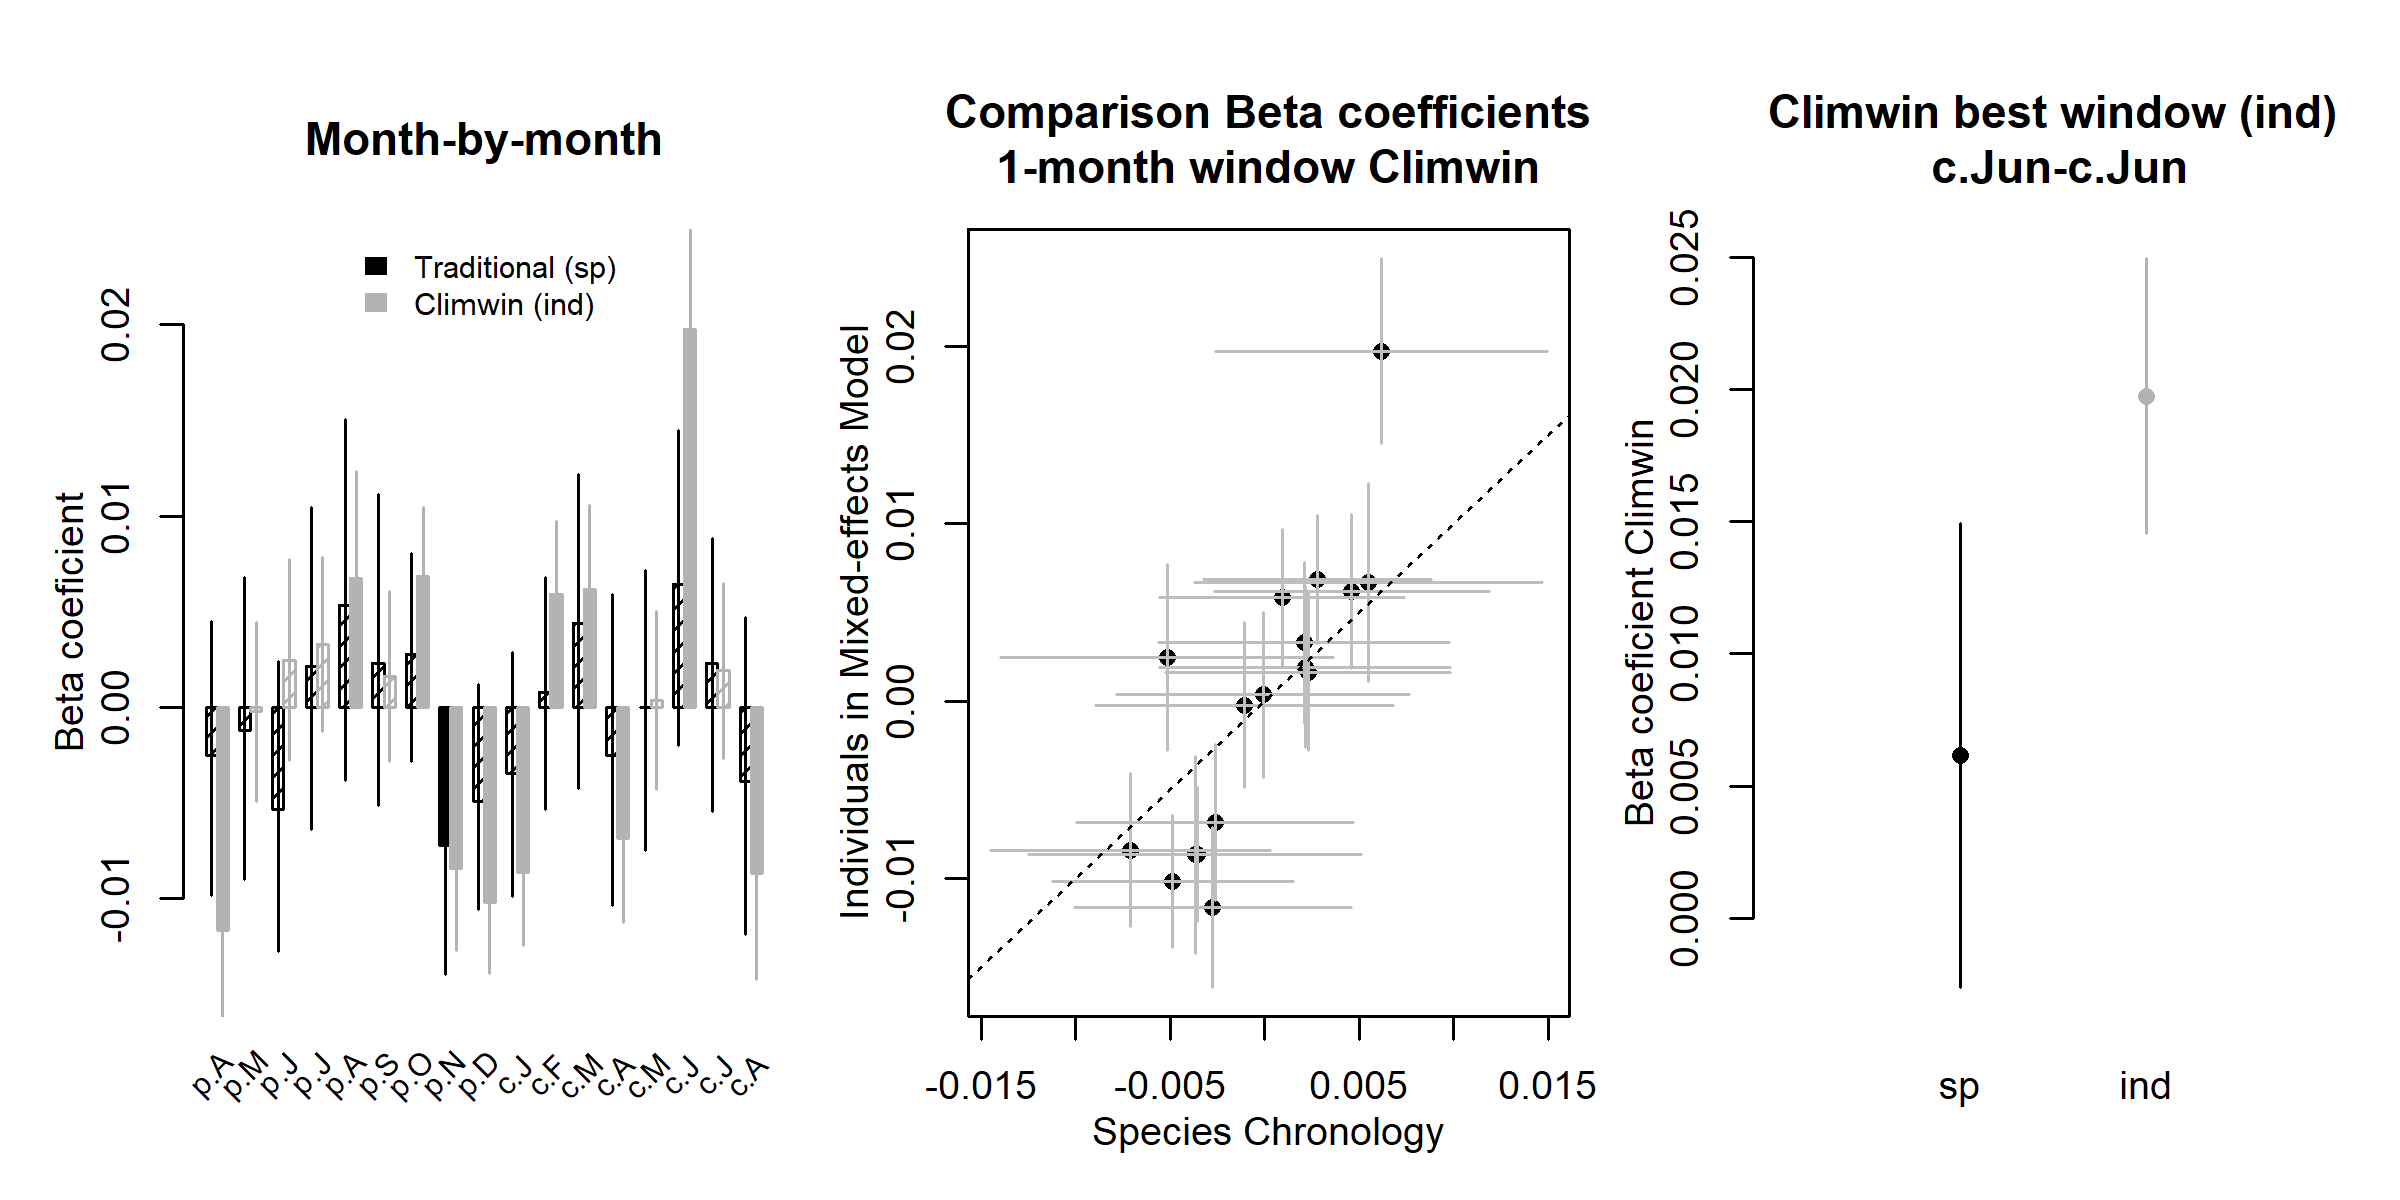
\includegraphics[width=0.95\textwidth,height=\textheight]{tables_figures/SI_figures/traditional_comparison/climwin_vs_dcc_Zofin_ABAL_wet.png}

\textbf{Maximum temperature}

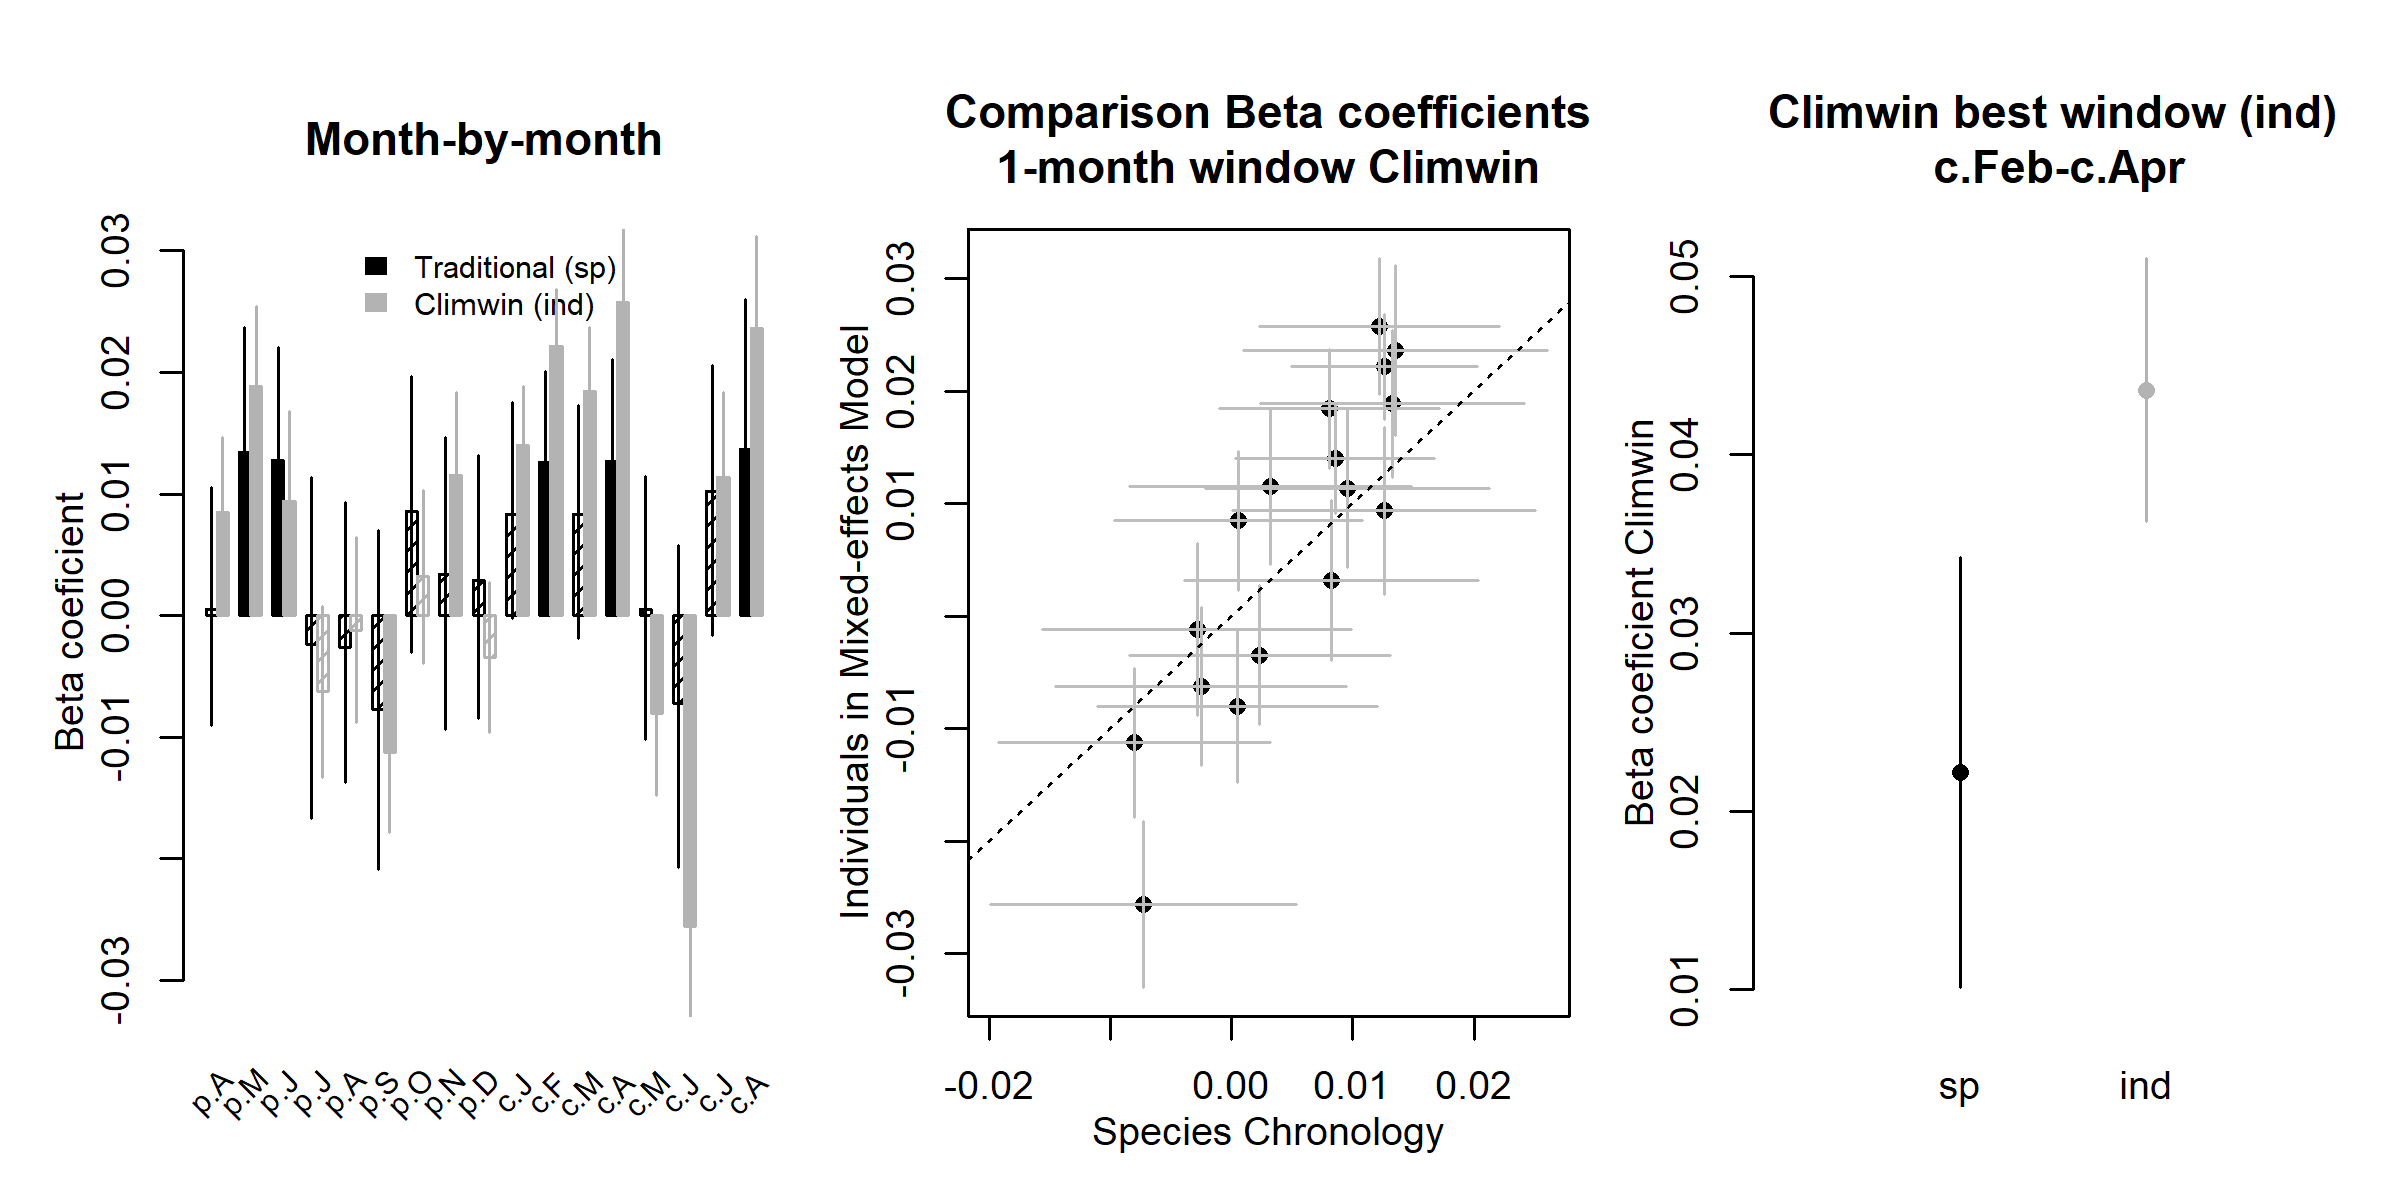
\includegraphics[width=0.95\textwidth,height=\textheight]{tables_figures/SI_figures/traditional_comparison/climwin_vs_dcc_Zofin_ABAL_tmx.png}

\textbf{Figure S2. Comparison of our approach with traditional methods
of identifying climate signals: ABAL at Zofin.} Shown are repsonses to
the precipitation- and temperature-group variables selected as most
influential by the \emph{climwin} analysis. Left panels show a
month-by-month comparison of \emph{beta} (slope) coefficients for the
relationship between tree growth and the monthly climate variable from
species-level residual chronologies (traditional approach) and from
individual-level analysis in \emph{climwin} (approach presented here).
Center panels compare the monthly \emph{beta} coefficient estimates,
with the dotted line indicating 1:1 correspondence. Finally, the right
panels compare \emph{beta} coefficients for the optimal window selected
by \emph{climwin}. Error bars indicate standard error of slope
estimates. Note that 1:1 correspondence is not necessarily expected. See
Appendix 5 for analysis methods and discussion of expected
correspondence.

\newpage

\hypertarget{figure-s3.-comparison-of-our-approach-with-traditional-methods-of-identifying-climate-signals-psme-at-cedar-breaks.}{%
\subsection{Figure S3. Comparison of our approach with traditional
methods of identifying climate signals: PSME at Cedar
Breaks.}\label{figure-s3.-comparison-of-our-approach-with-traditional-methods-of-identifying-climate-signals-psme-at-cedar-breaks.}}

\textbf{Precipitation}

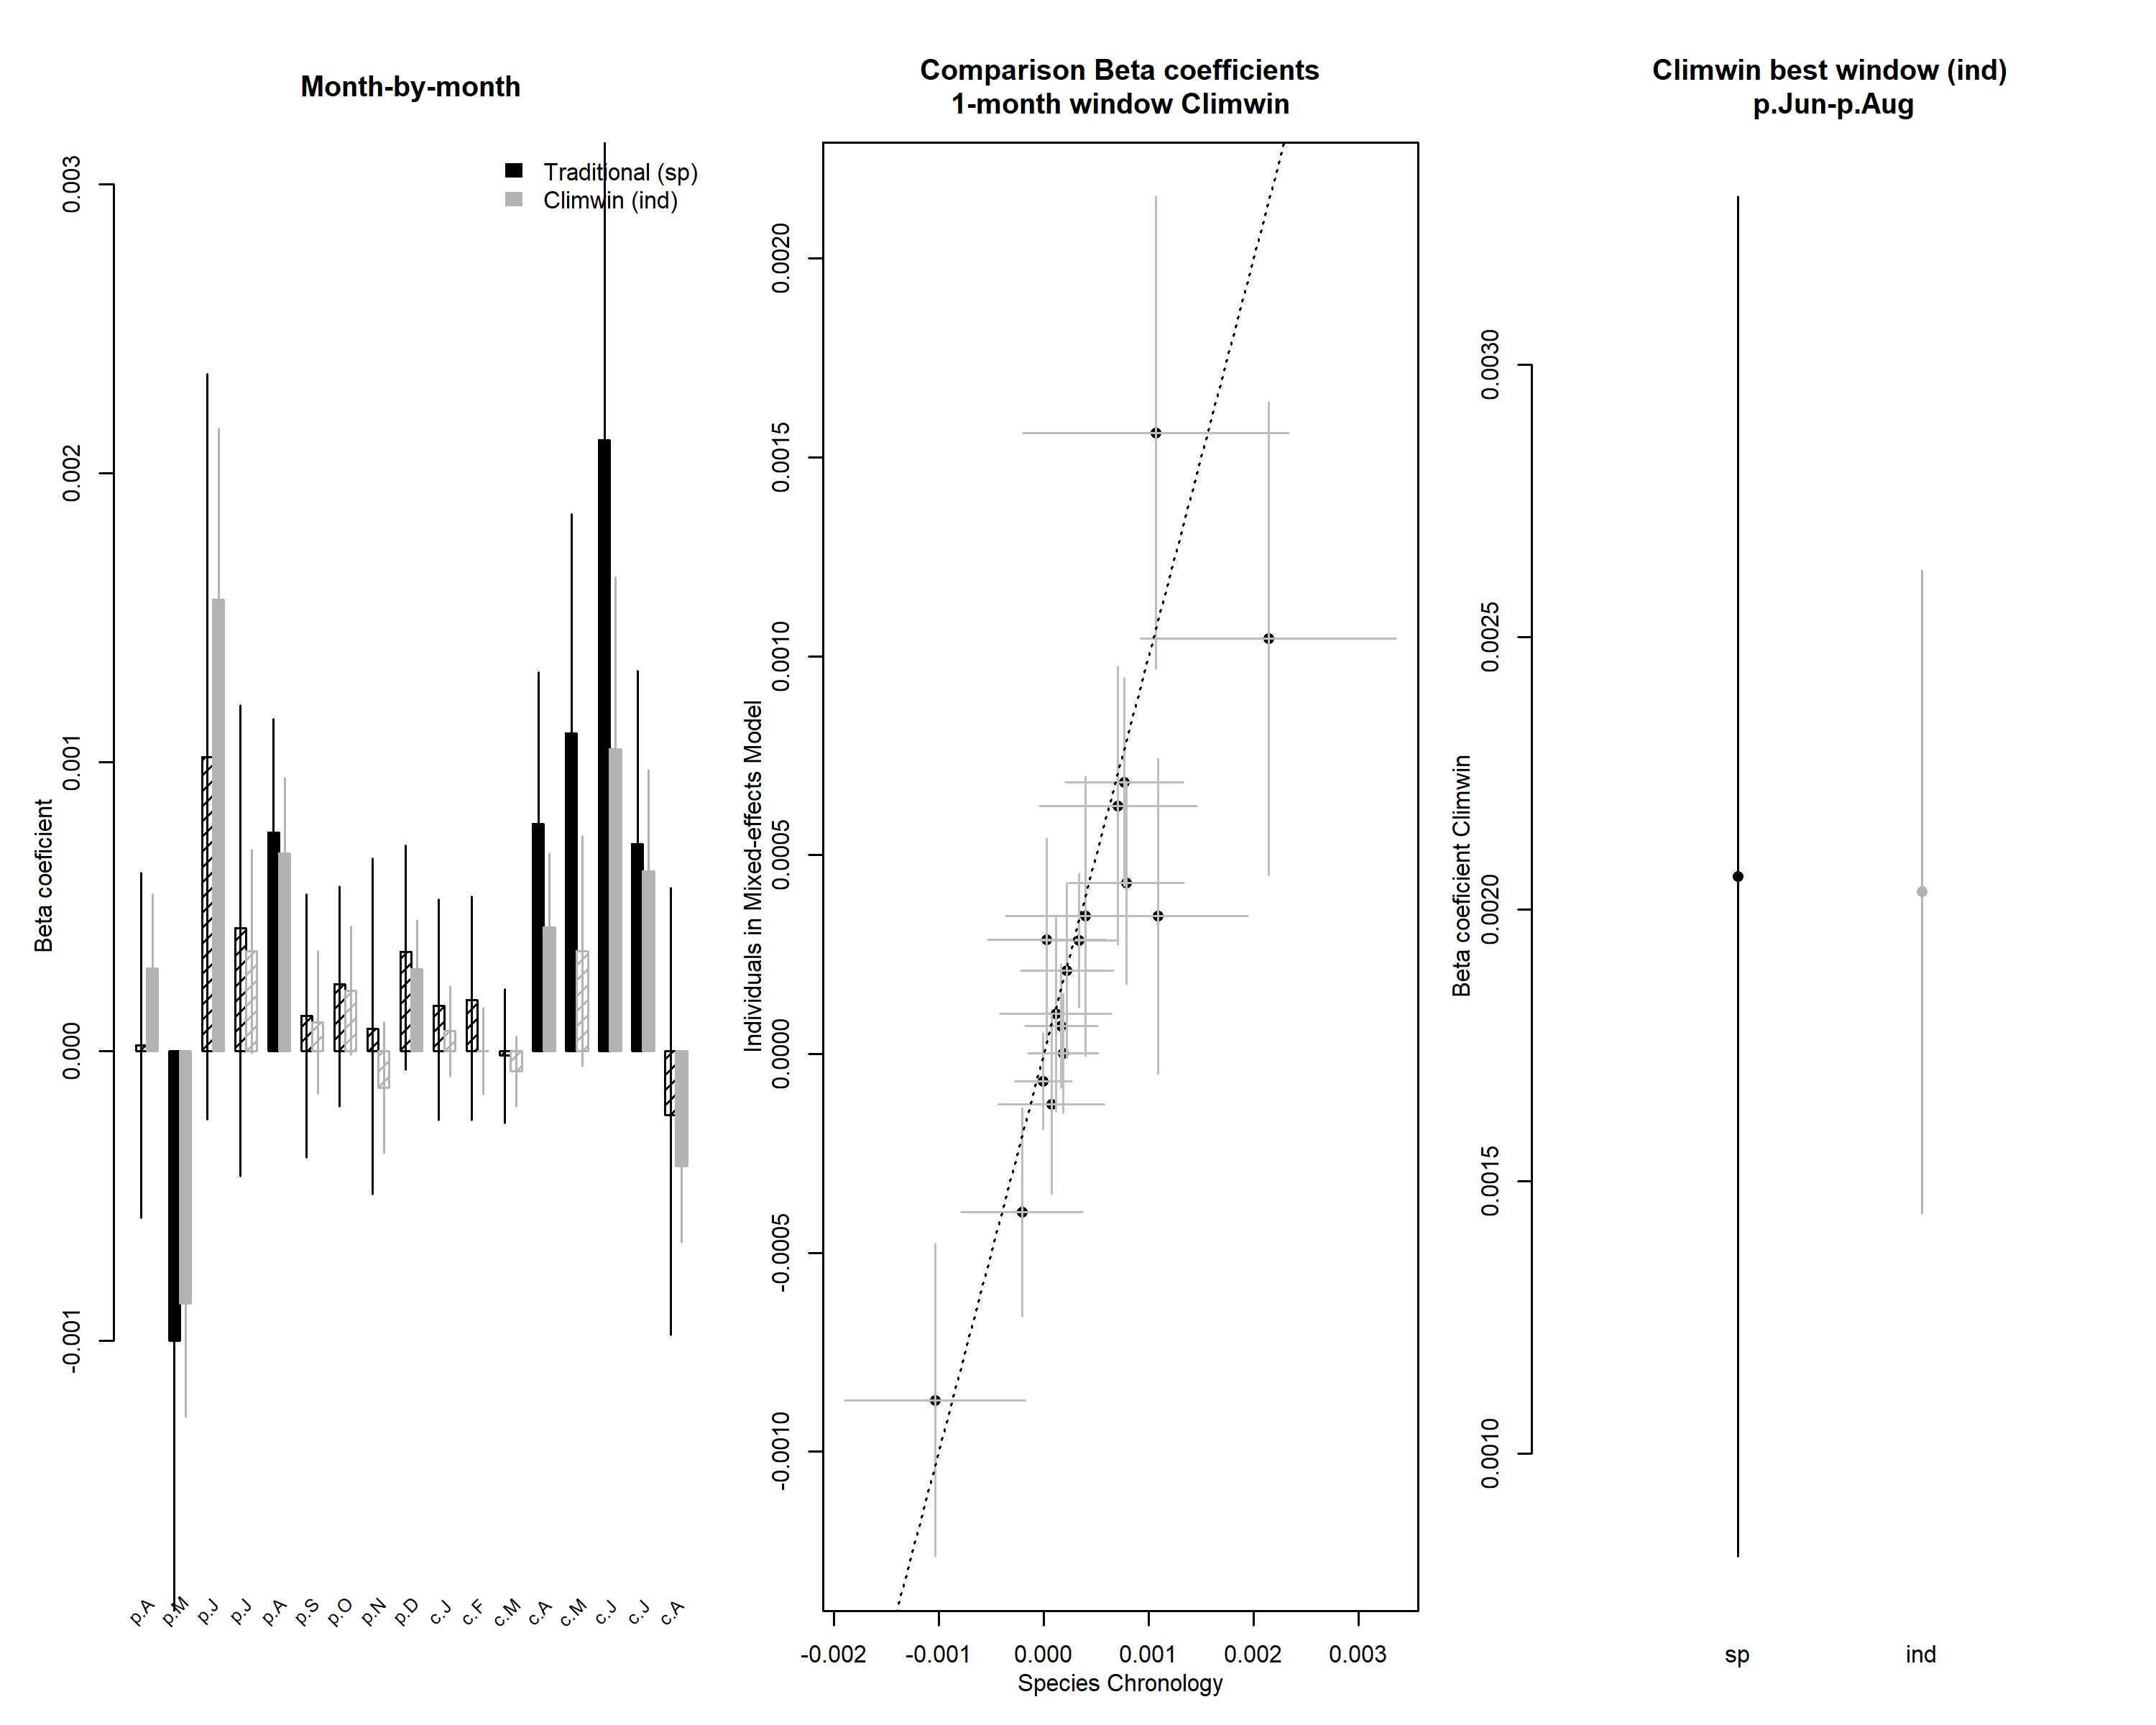
\includegraphics[width=0.95\textwidth,height=\textheight]{tables_figures/SI_figures/traditional_comparison/climwin_vs_dcc_CedarBreaks_PSME_pre.png}

\textbf{Maximum temperature}

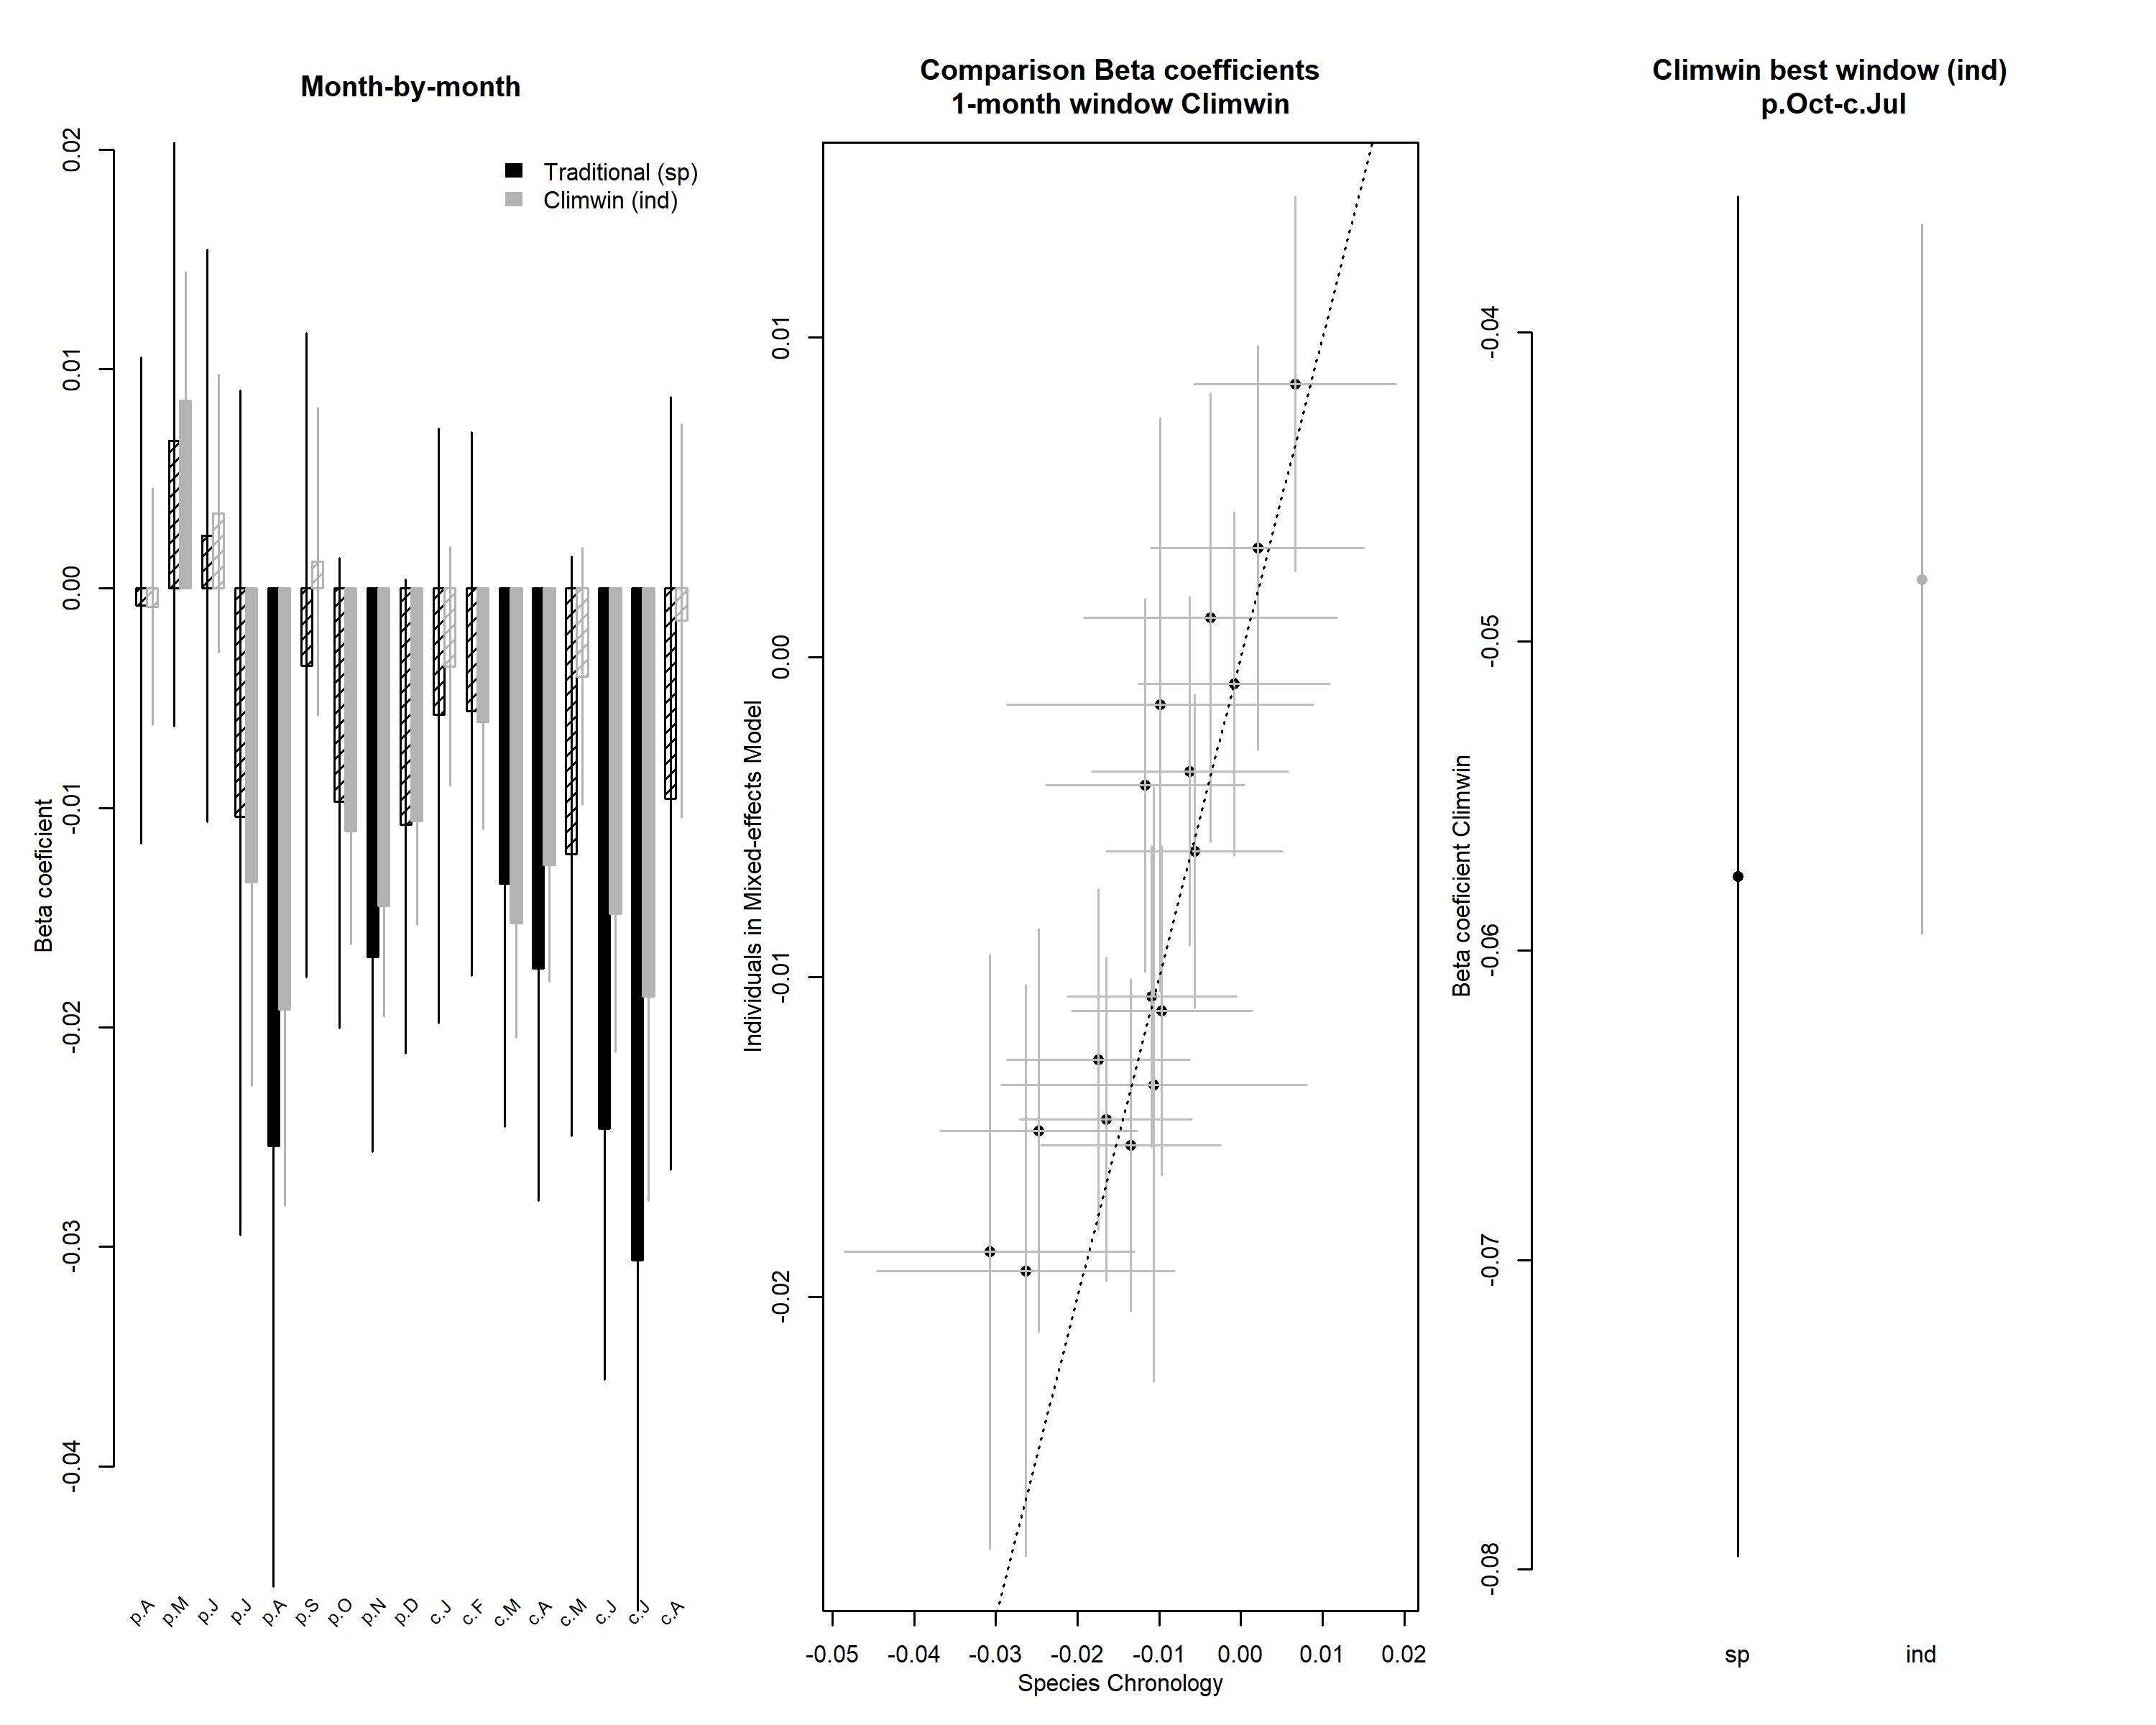
\includegraphics[width=0.95\textwidth,height=\textheight]{tables_figures/SI_figures/traditional_comparison/climwin_vs_dcc_CedarBreaks_PSME_tmx.png}

\textbf{Figure S3. Comparison of our approach with traditional methods
of identifying climate signals: PSME at Cedar Breaks.} Shown are
repsonses to the precipitation- and temperature-group variables selected
as most influential by the \emph{climwin} analysis. Left panels show a
month-by-month comparison of \emph{beta} (slope) coefficients for the
relationship between tree growth and the monthly climate variable from
species-level residual chronologies (traditional approach) and from
individual-level analysis in \emph{climwin} (approach presented here).
Center panels compare the monthly \emph{beta} coefficient estimates,
with the dotted line indicating 1:1 correspondence. Finally, the right
panels compare \emph{beta} coefficients for the optimal window selected
by \emph{climwin}. Error bars indicate standard error of slope
estimates. Note that 1:1 correspondence is not necessarily expected. See
Appendix 5 for analysis methods and discussion of expected
correspondence.

\newpage

\hypertarget{figure-s4.-comparison-of-our-approach-with-traditional-methods-of-identifying-climate-signals-pima-at-scotty-creek.}{%
\subsection{Figure S4. Comparison of our approach with traditional
methods of identifying climate signals: PIMA at Scotty
Creek.}\label{figure-s4.-comparison-of-our-approach-with-traditional-methods-of-identifying-climate-signals-pima-at-scotty-creek.}}

\textbf{Precipitation}

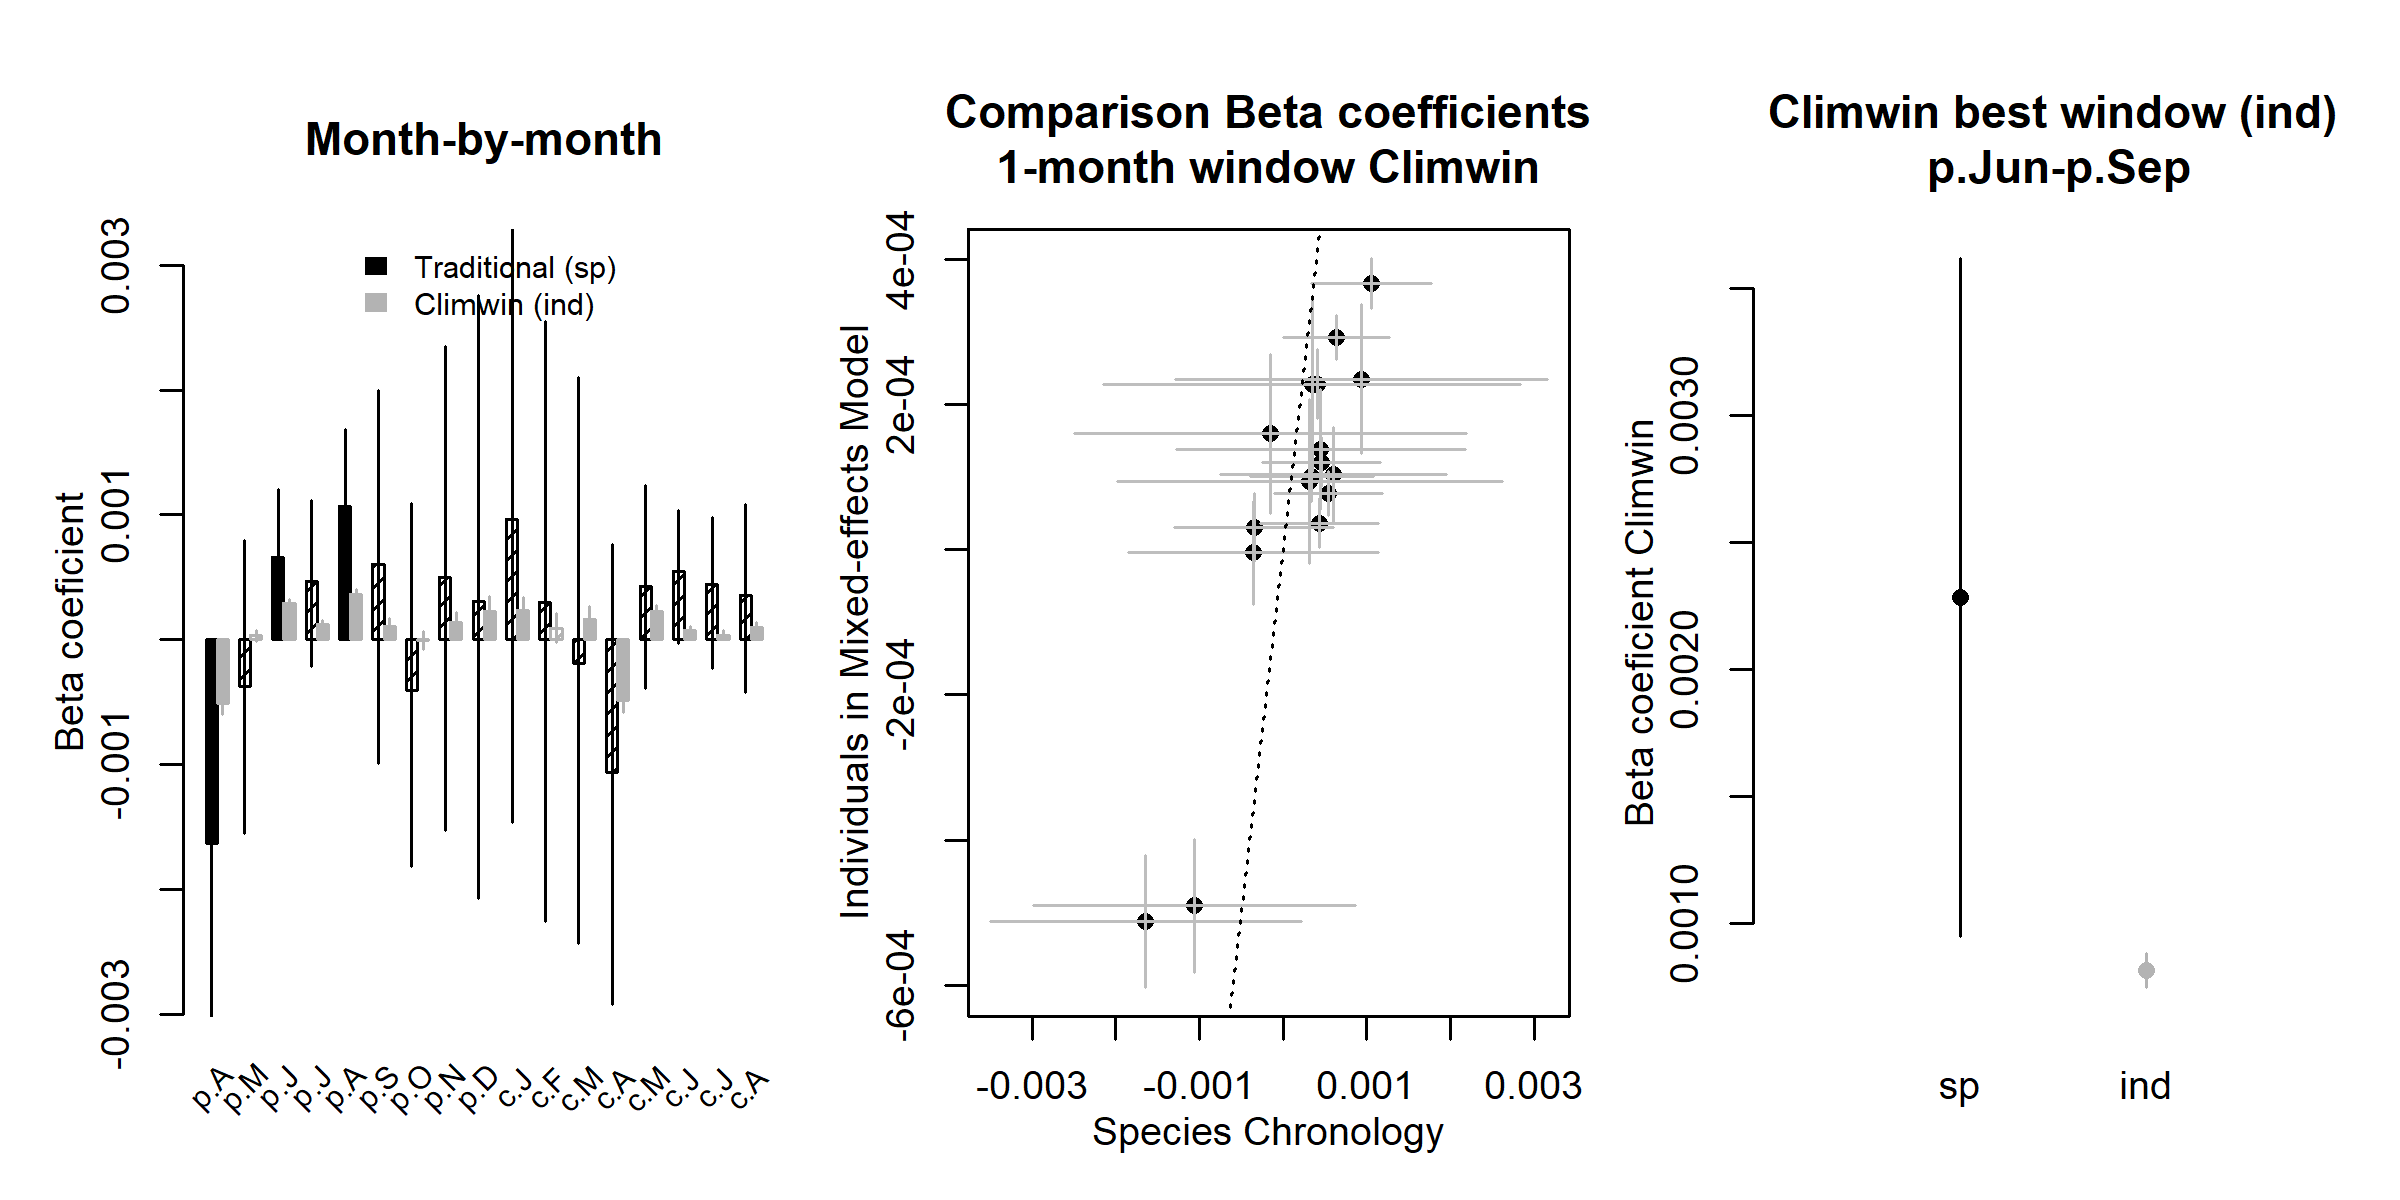
\includegraphics[width=0.95\textwidth,height=\textheight]{tables_figures/SI_figures/traditional_comparison/climwin_vs_dcc_ScottyCreek_PIMA_pre.png}

\textbf{Maximum temperature}

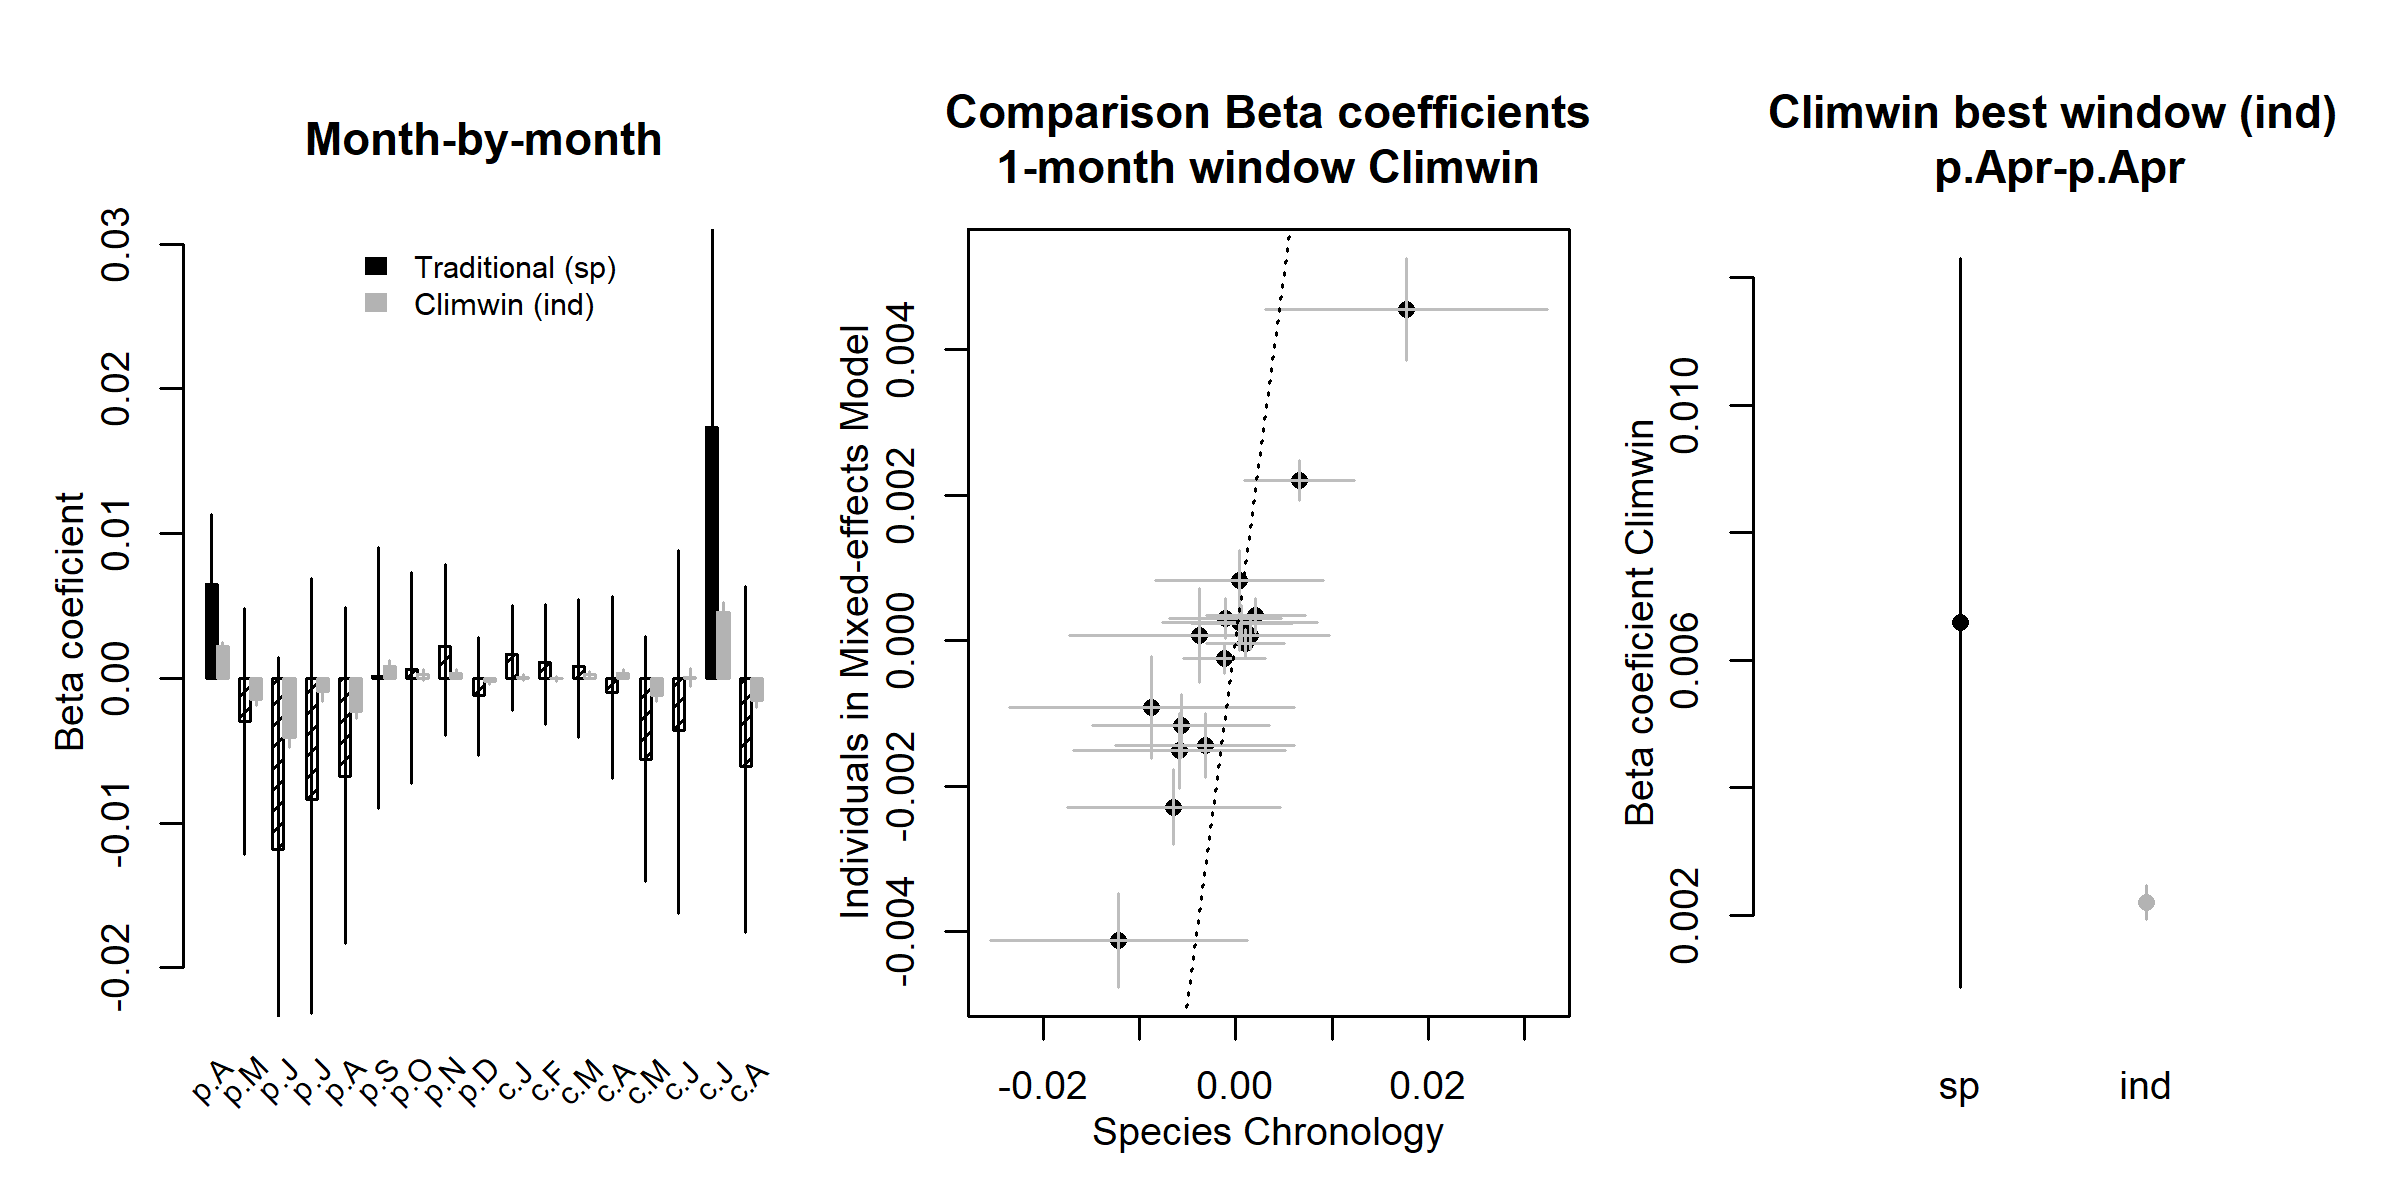
\includegraphics[width=0.95\textwidth,height=\textheight]{tables_figures/SI_figures/traditional_comparison/climwin_vs_dcc_ScottyCreek_PIMA_tmx.png}

\textbf{Figure S4. Comparison of our approach with traditional methods
of identifying climate signals: PIMA at Scotty Creek.} Shown are
repsonses to the precipitation- and temperature-group variables selected
as most influential by the \emph{climwin} analysis. Left panels show a
month-by-month comparison of \emph{beta} (slope) coefficients for the
relationship between tree growth and the monthly climate variable from
species-level residual chronologies (traditional approach) and from
individual-level analysis in \emph{climwin} (approach presented here).
Center panels compare the monthly \emph{beta} coefficient estimates,
with the dotted line indicating 1:1 correspondence. Finally, the right
panels compare \emph{beta} coefficients for the optimal window selected
by \emph{climwin}. Error bars indicate standard error of slope
estimates. Note that 1:1 correspondence is not necessarily expected. See
Appendix 5 for analysis methods and discussion of expected
correspondence.

\newpage

\hypertarget{figure-s5.-pre-at-scbi}{%
\subsection{Figure S5. (PRE at SCBI)}\label{figure-s5.-pre-at-scbi}}

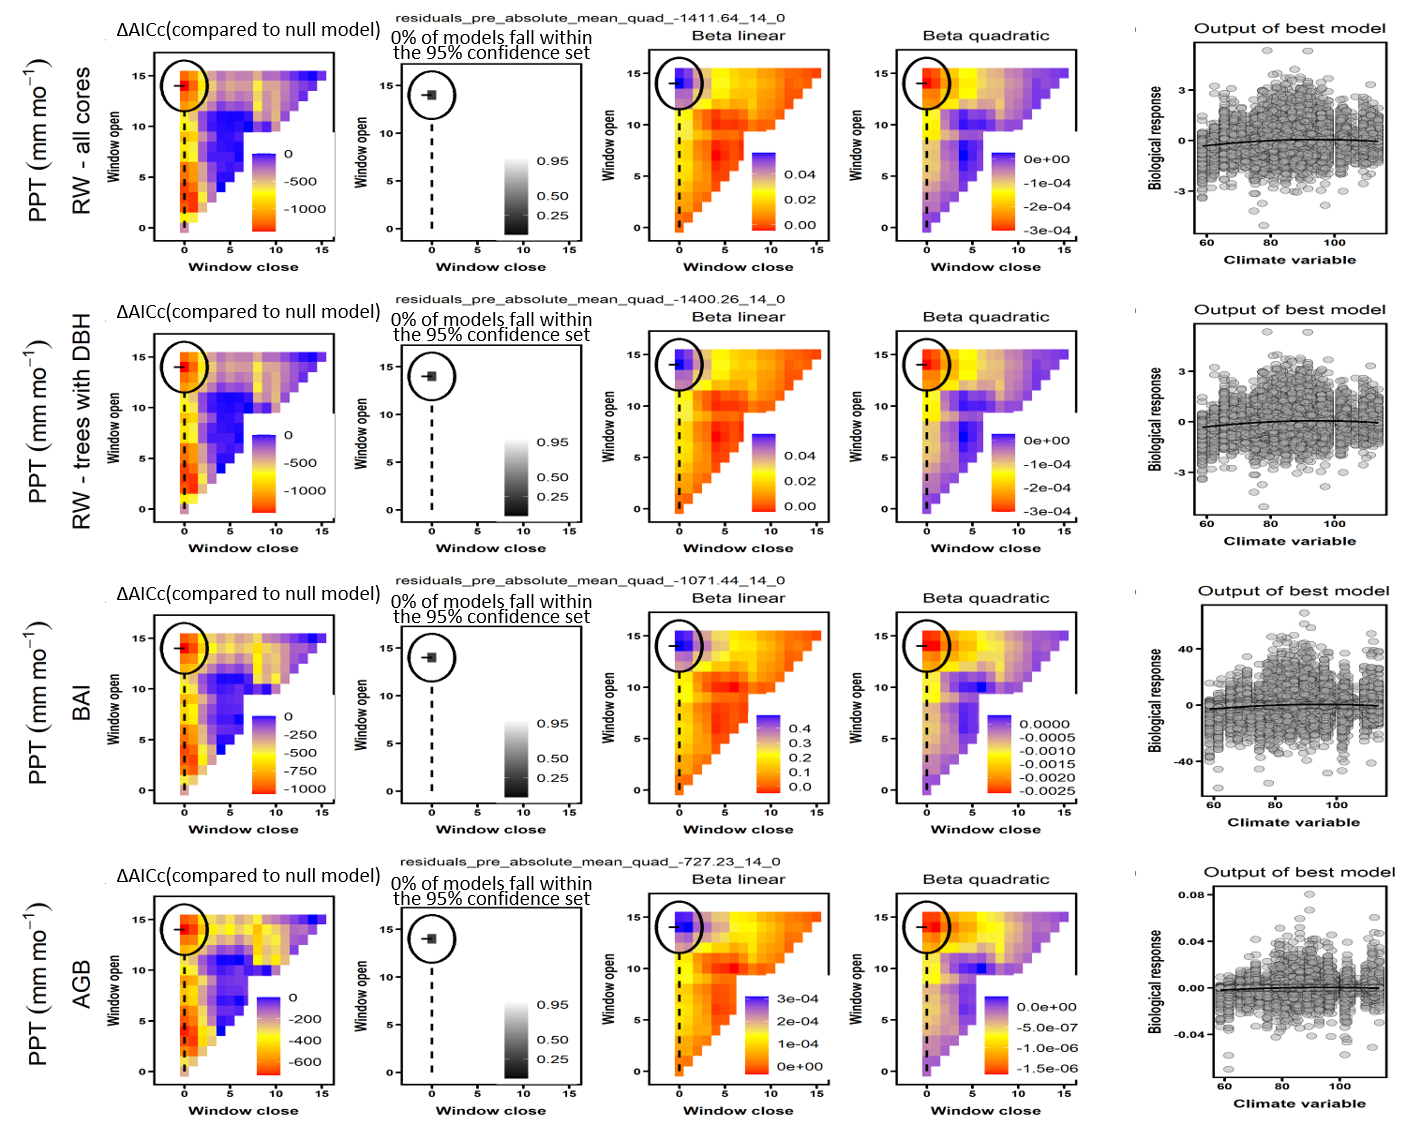
\includegraphics{tables_figures/SI_figures/climwin_plots_combined/SCBI_pre.png}

\textbf{Figure S5. (PRE at SCBI)} Here, \emph{climwin} identified
\textbf{GIVE WINDOW} precipitation (\(PPT\)) as the strongest climate
variable across all four analyses (\(RW\) with and without trees for
which \(DBH\) could not be reconstructed, \(BAI\), \(\Delta AGB\)).

\newpage

\hypertarget{figure-s6.-pet-at-scbi}{%
\subsection{Figure S6. (PET at SCBI)}\label{figure-s6.-pet-at-scbi}}

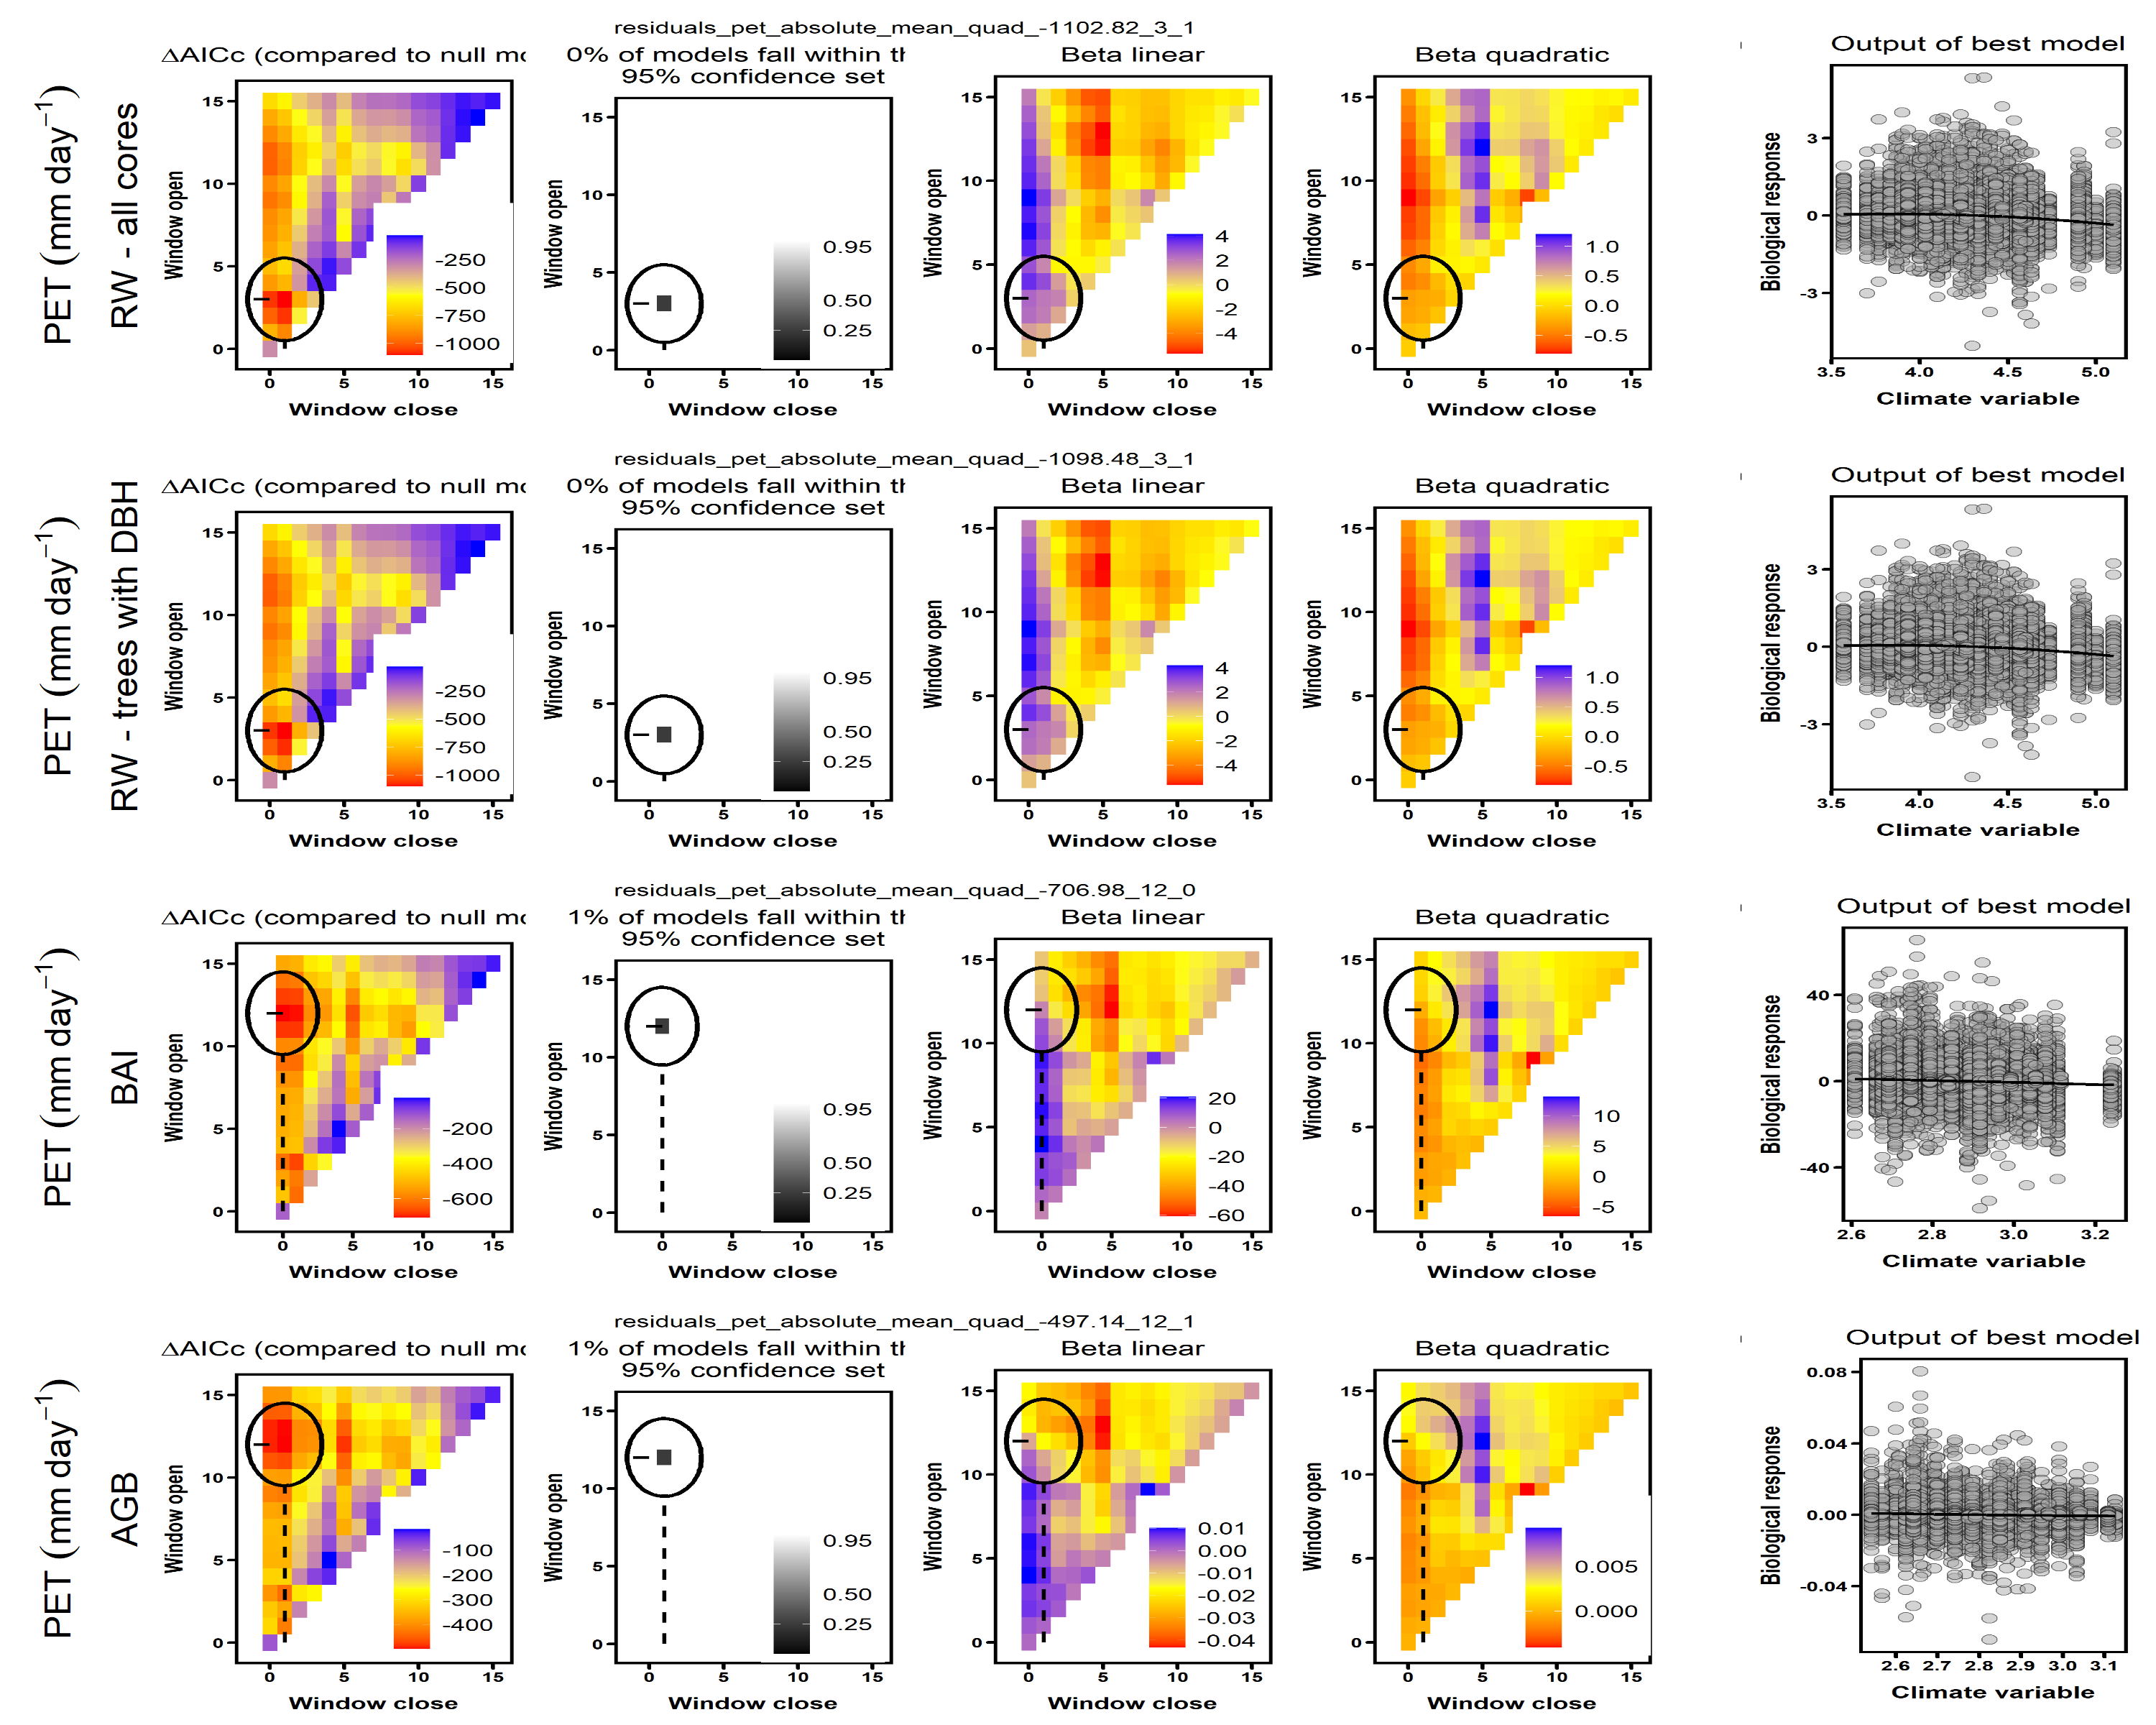
\includegraphics{tables_figures/SI_figures/climwin_plots_combined/SCBI_pet.png}

\textbf{Figure S6. (PET at SCBI)} Here, \emph{climwin} identified
potential evapotranspiration (\(PET\)) as the strongest climate variable
across all four analyses (\(RW\) with and without trees for which
\(DBH\) could not be reconstructed, \(BAI\), \(\Delta AGB\)), but a
different window (\textbf{GIVE WINDOW}) was chosen for \(BAI\) and
\(\Delta AGB\) than for \(RW\) (\textbf{GIVE WINDOW}).

\newpage

\hypertarget{figure-s7.-tmptmn-at-bci}{%
\subsection{Figure S7. (TMP/TMN at
BCI)}\label{figure-s7.-tmptmn-at-bci}}

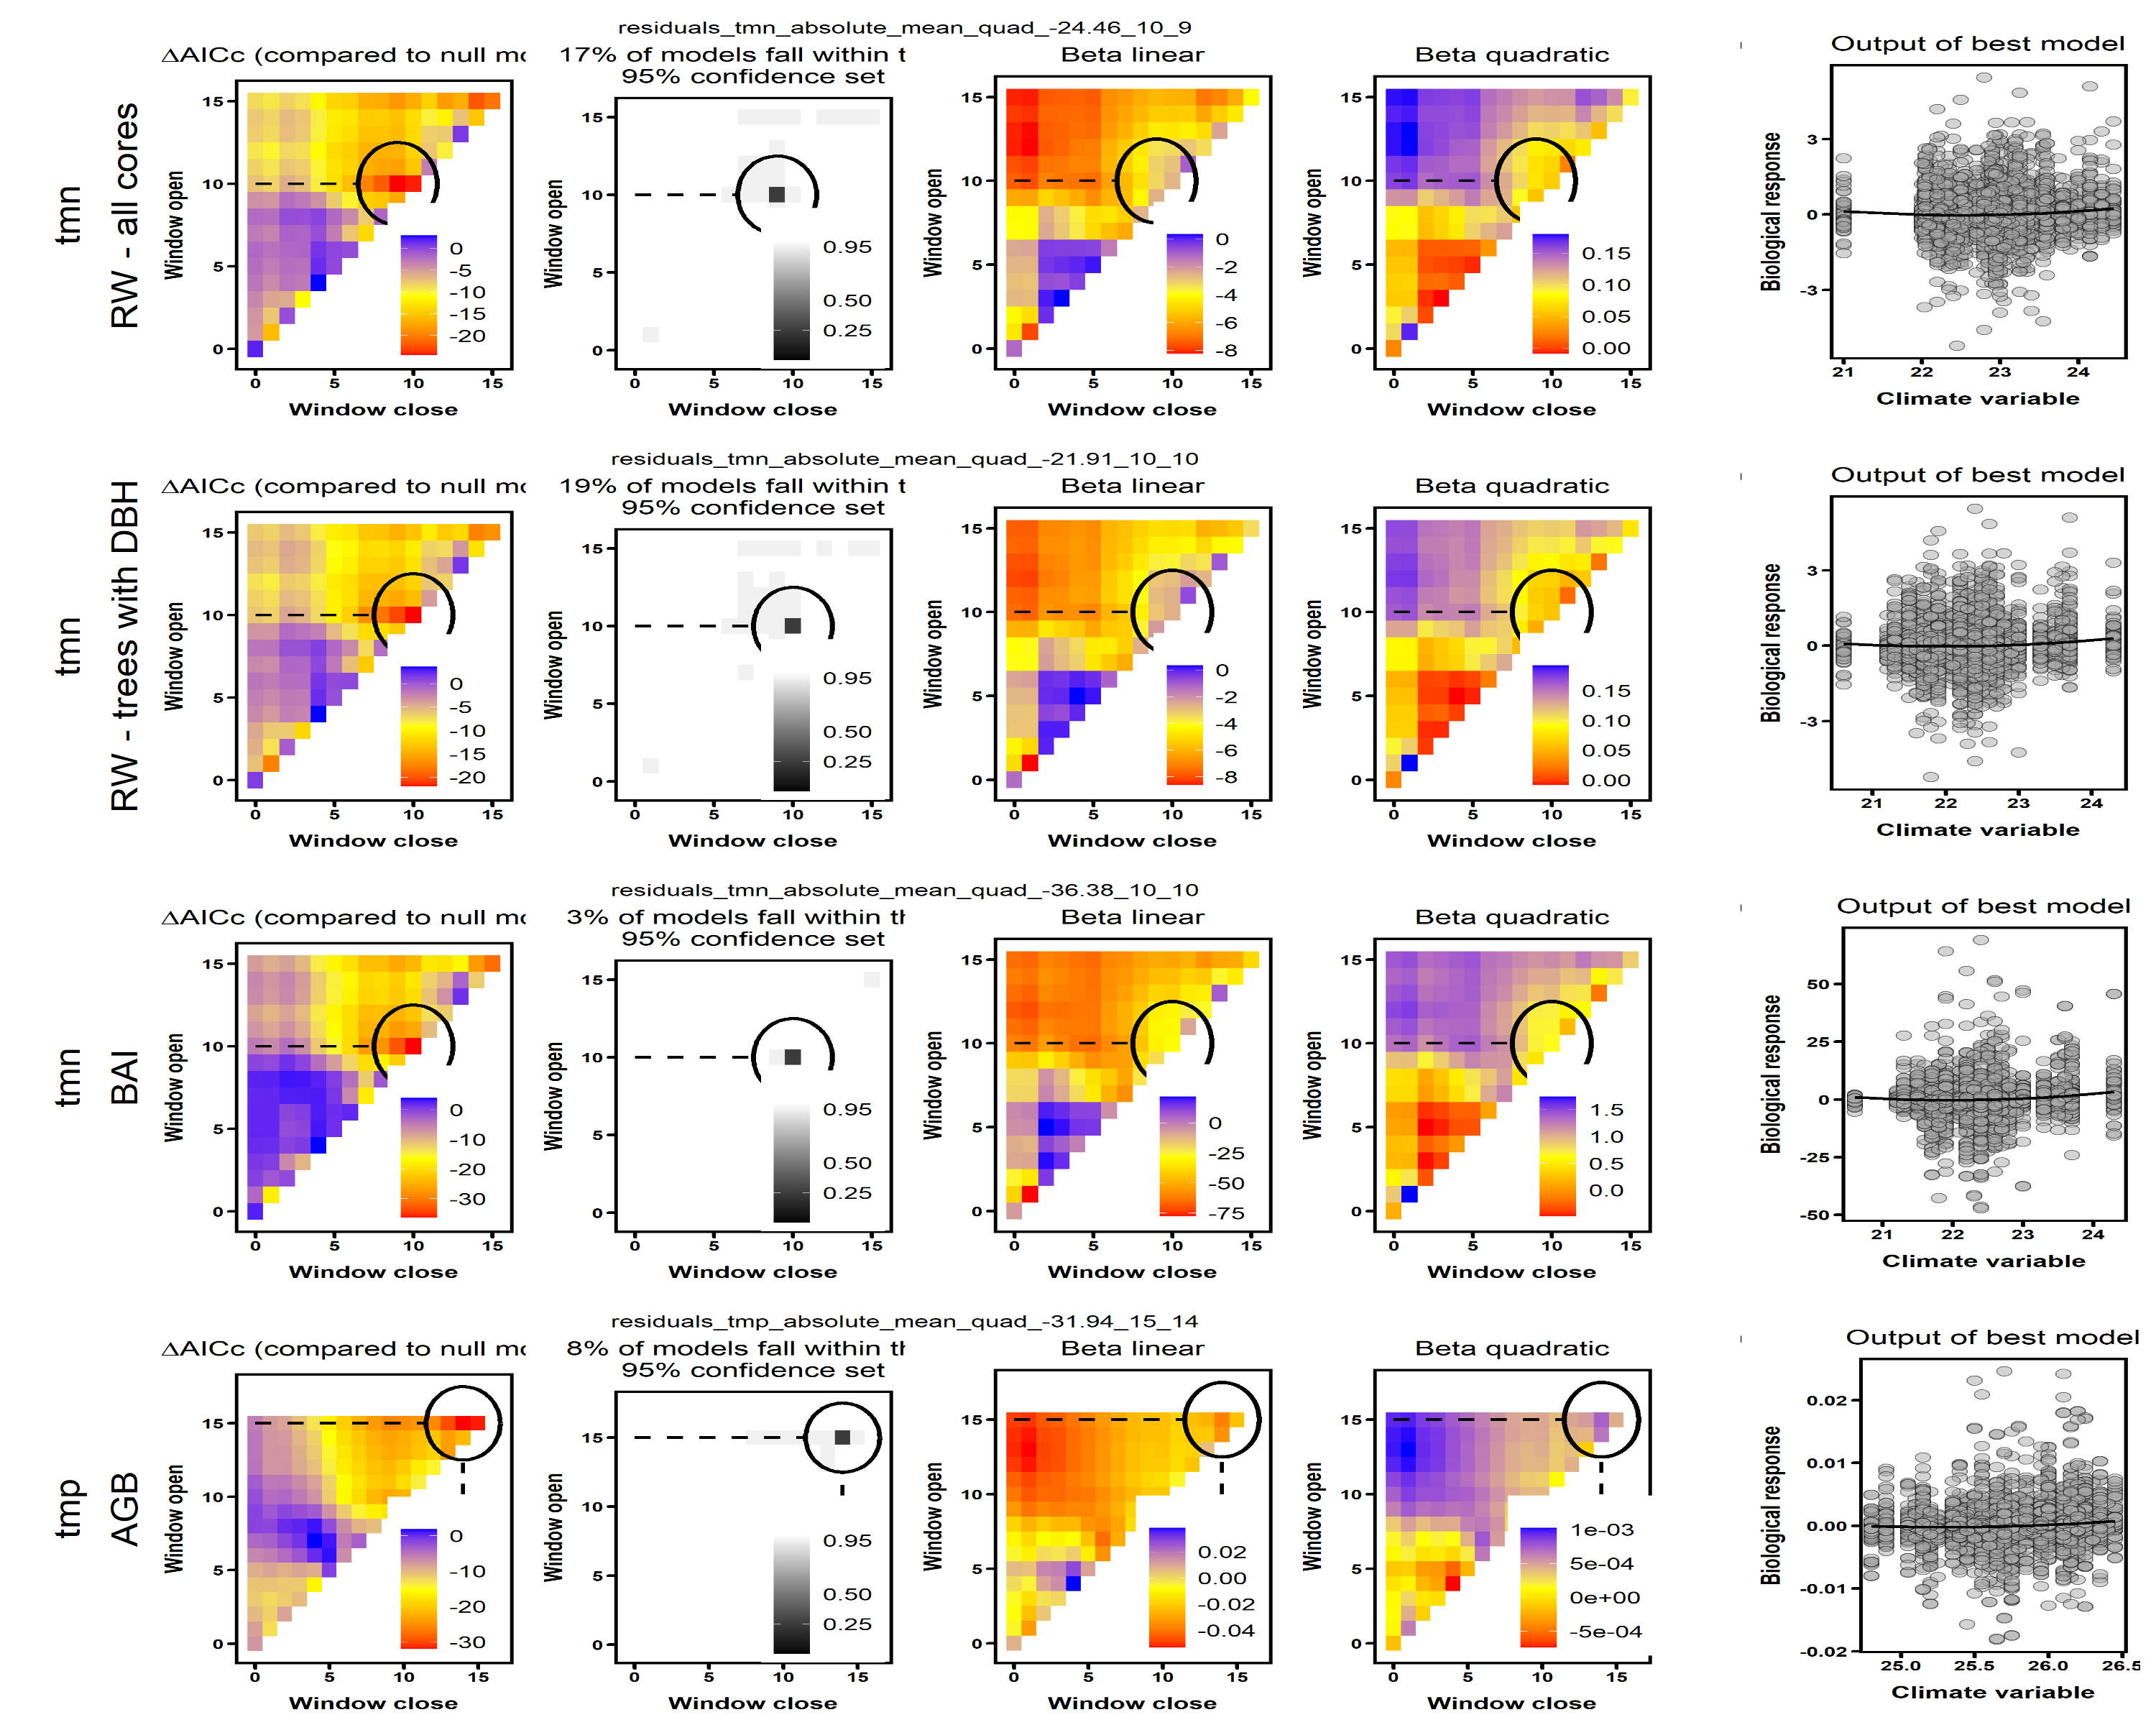
\includegraphics{tables_figures/SI_figures/climwin_plots_combined/BCI_tmp_tmn.png}

\textbf{Figure S7. (TMP/TMN at BCI)} Here\ldots.

\newpage

\hypertarget{figure-s9.-best-gls-models-for-barro-colorado-island-panama}{%
\subsection{Figure S9. Best GLS models for Barro Colorado Island
(Panama)}\label{figure-s9.-best-gls-models-for-barro-colorado-island-panama}}

\begin{figure}
\centering
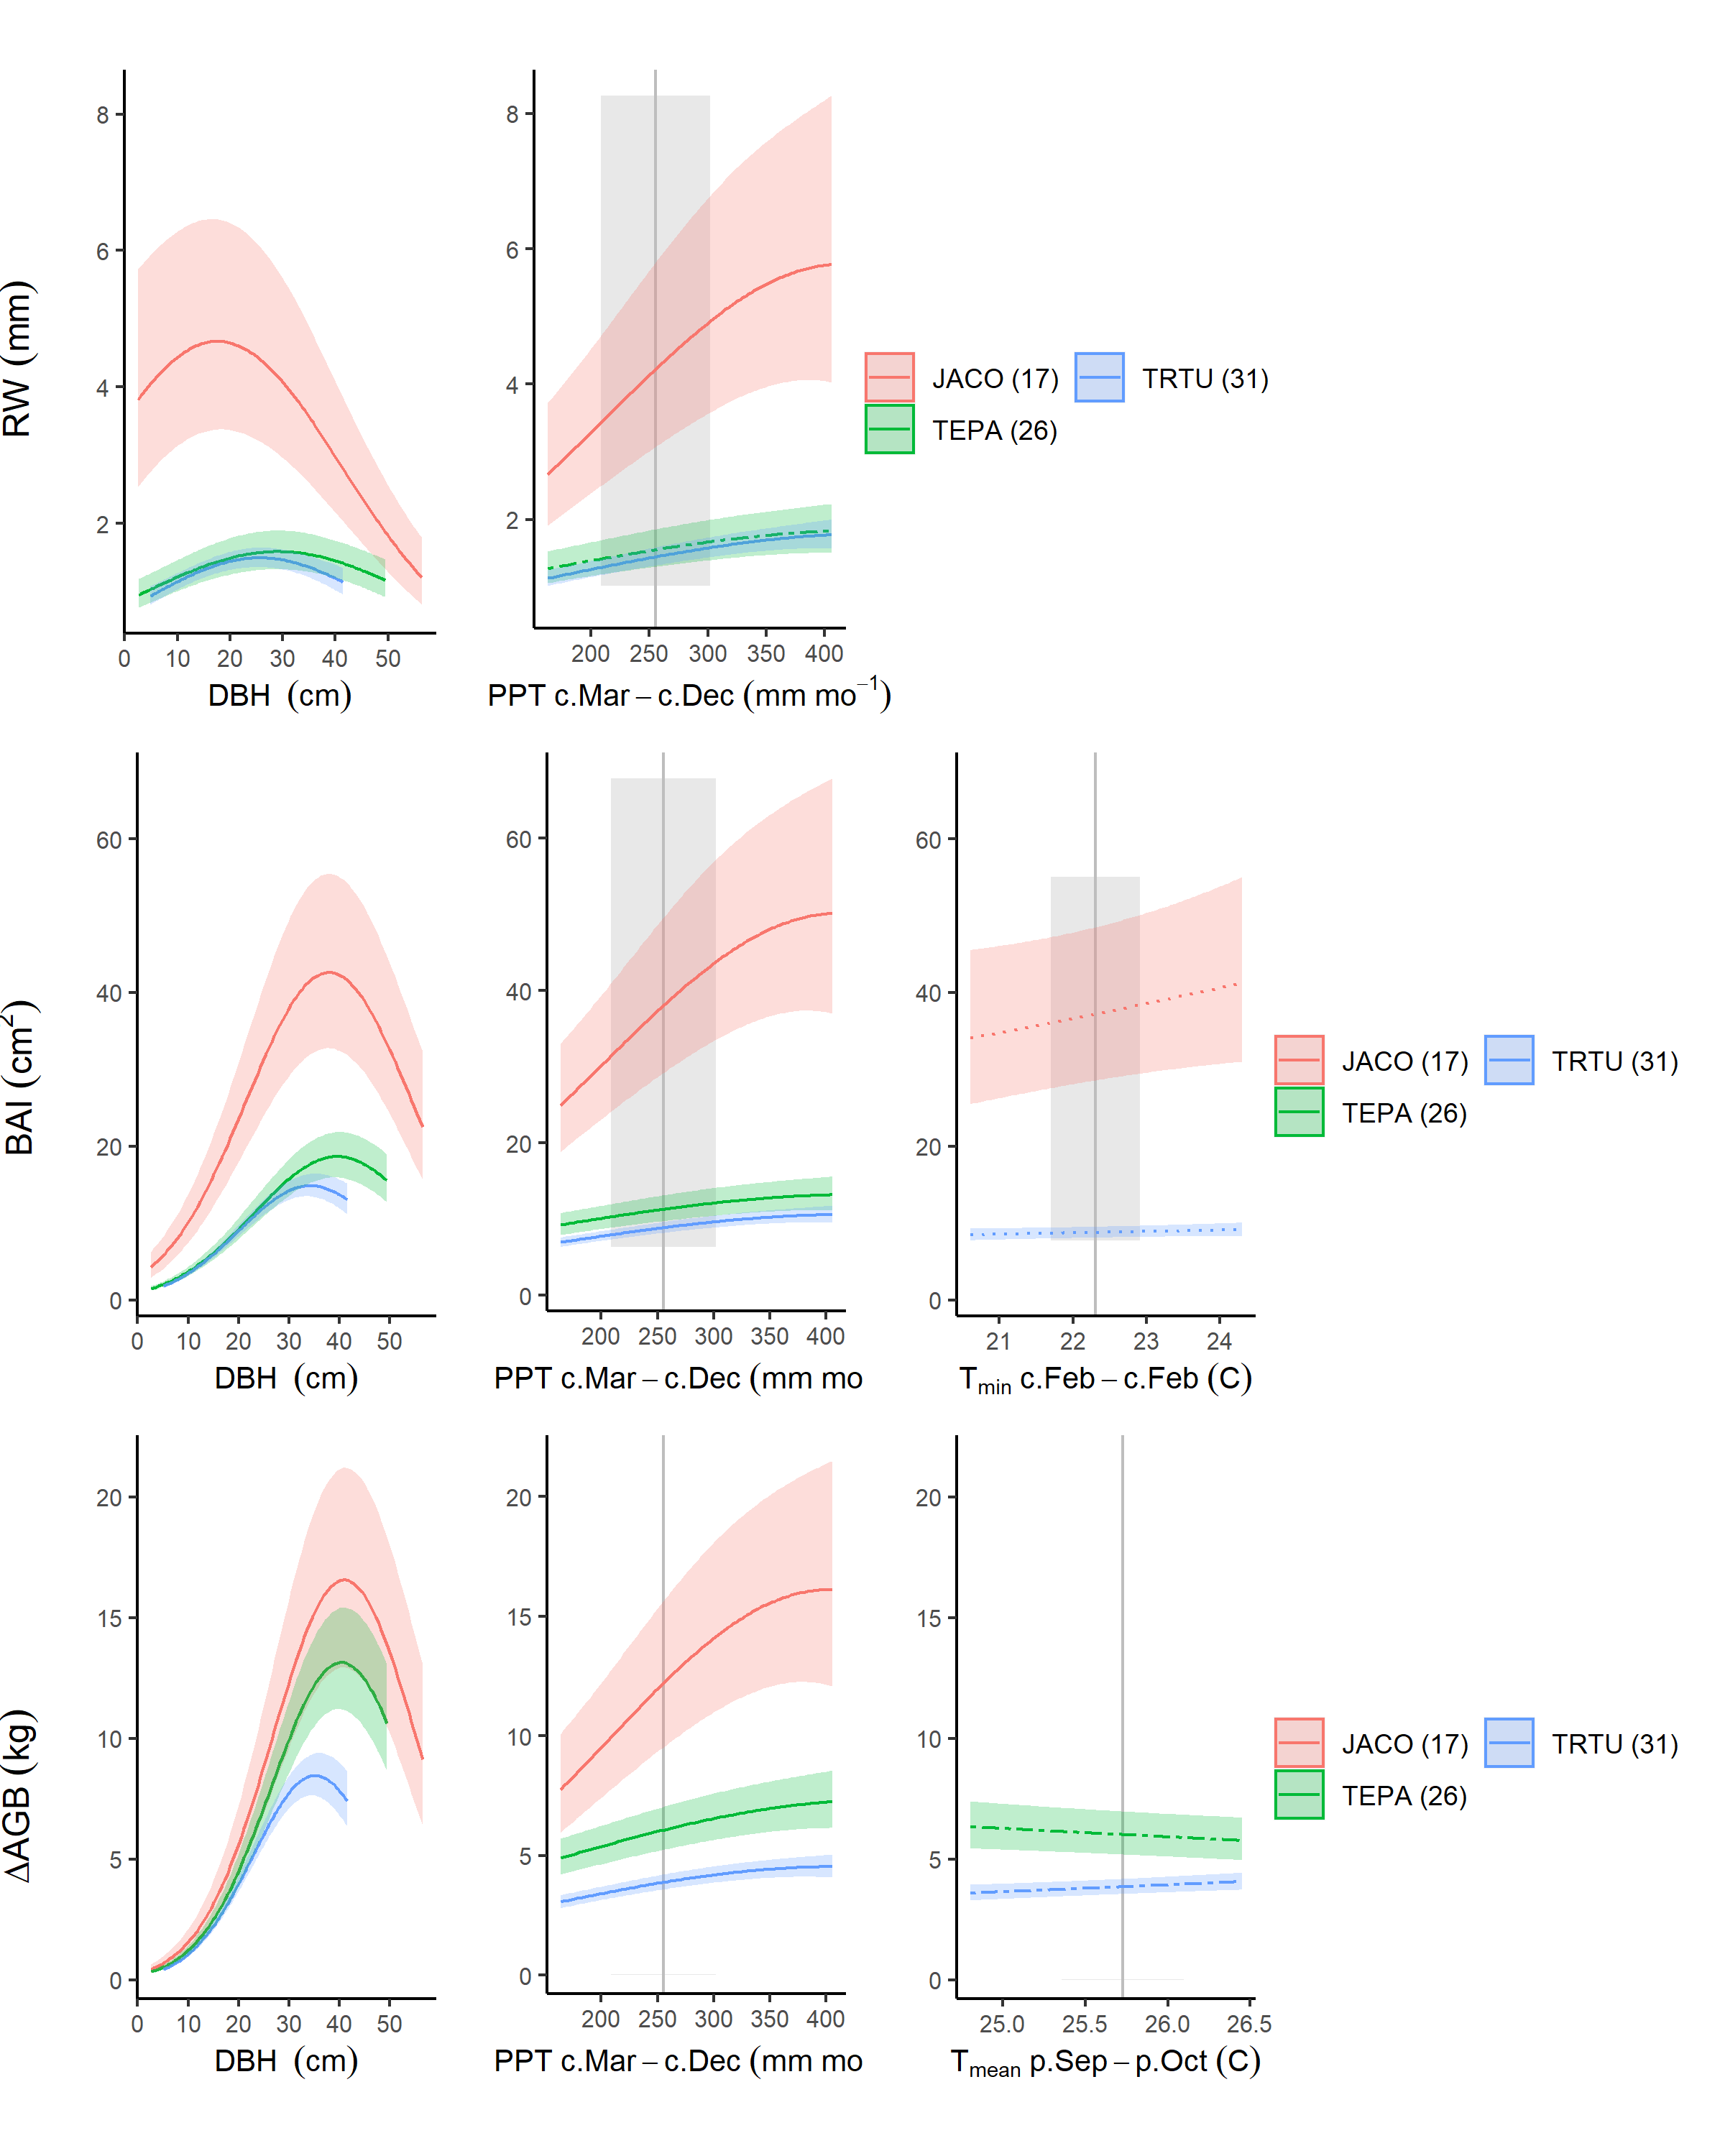
\includegraphics[width=0.75\textwidth,height=\textheight]{tables_figures/SI_figures/composite_plots/BCI.png}
\caption{Figure S9. Best GLS models for Barro Colorado Island (Panama)
for all three growth metrics examined here. Precipitation and
temperature group variables are as selected by \emph{climwin}
(p=previous year, c=current year). For each species, relationships are
plotted if included in top model, with best-fit polynomials plotted with
solid lines when both first- and second-order terms are signficant,
dashed lines when only one term is signficant, and dotted lines when
neither is signficant. Transparent ribbons indicate 95\% confidence
intervals. Vertical grey lines indicate the long-term mean for the
climate variable, shading indicates 1 SD.}
\end{figure}

\newpage

\hypertarget{figure-s10.-best-gls-models-for-huai-kha-khaeng-thailand}{%
\subsection{Figure S10. Best GLS models for Huai Kha Khaeng
(Thailand)}\label{figure-s10.-best-gls-models-for-huai-kha-khaeng-thailand}}

\begin{figure}
\centering
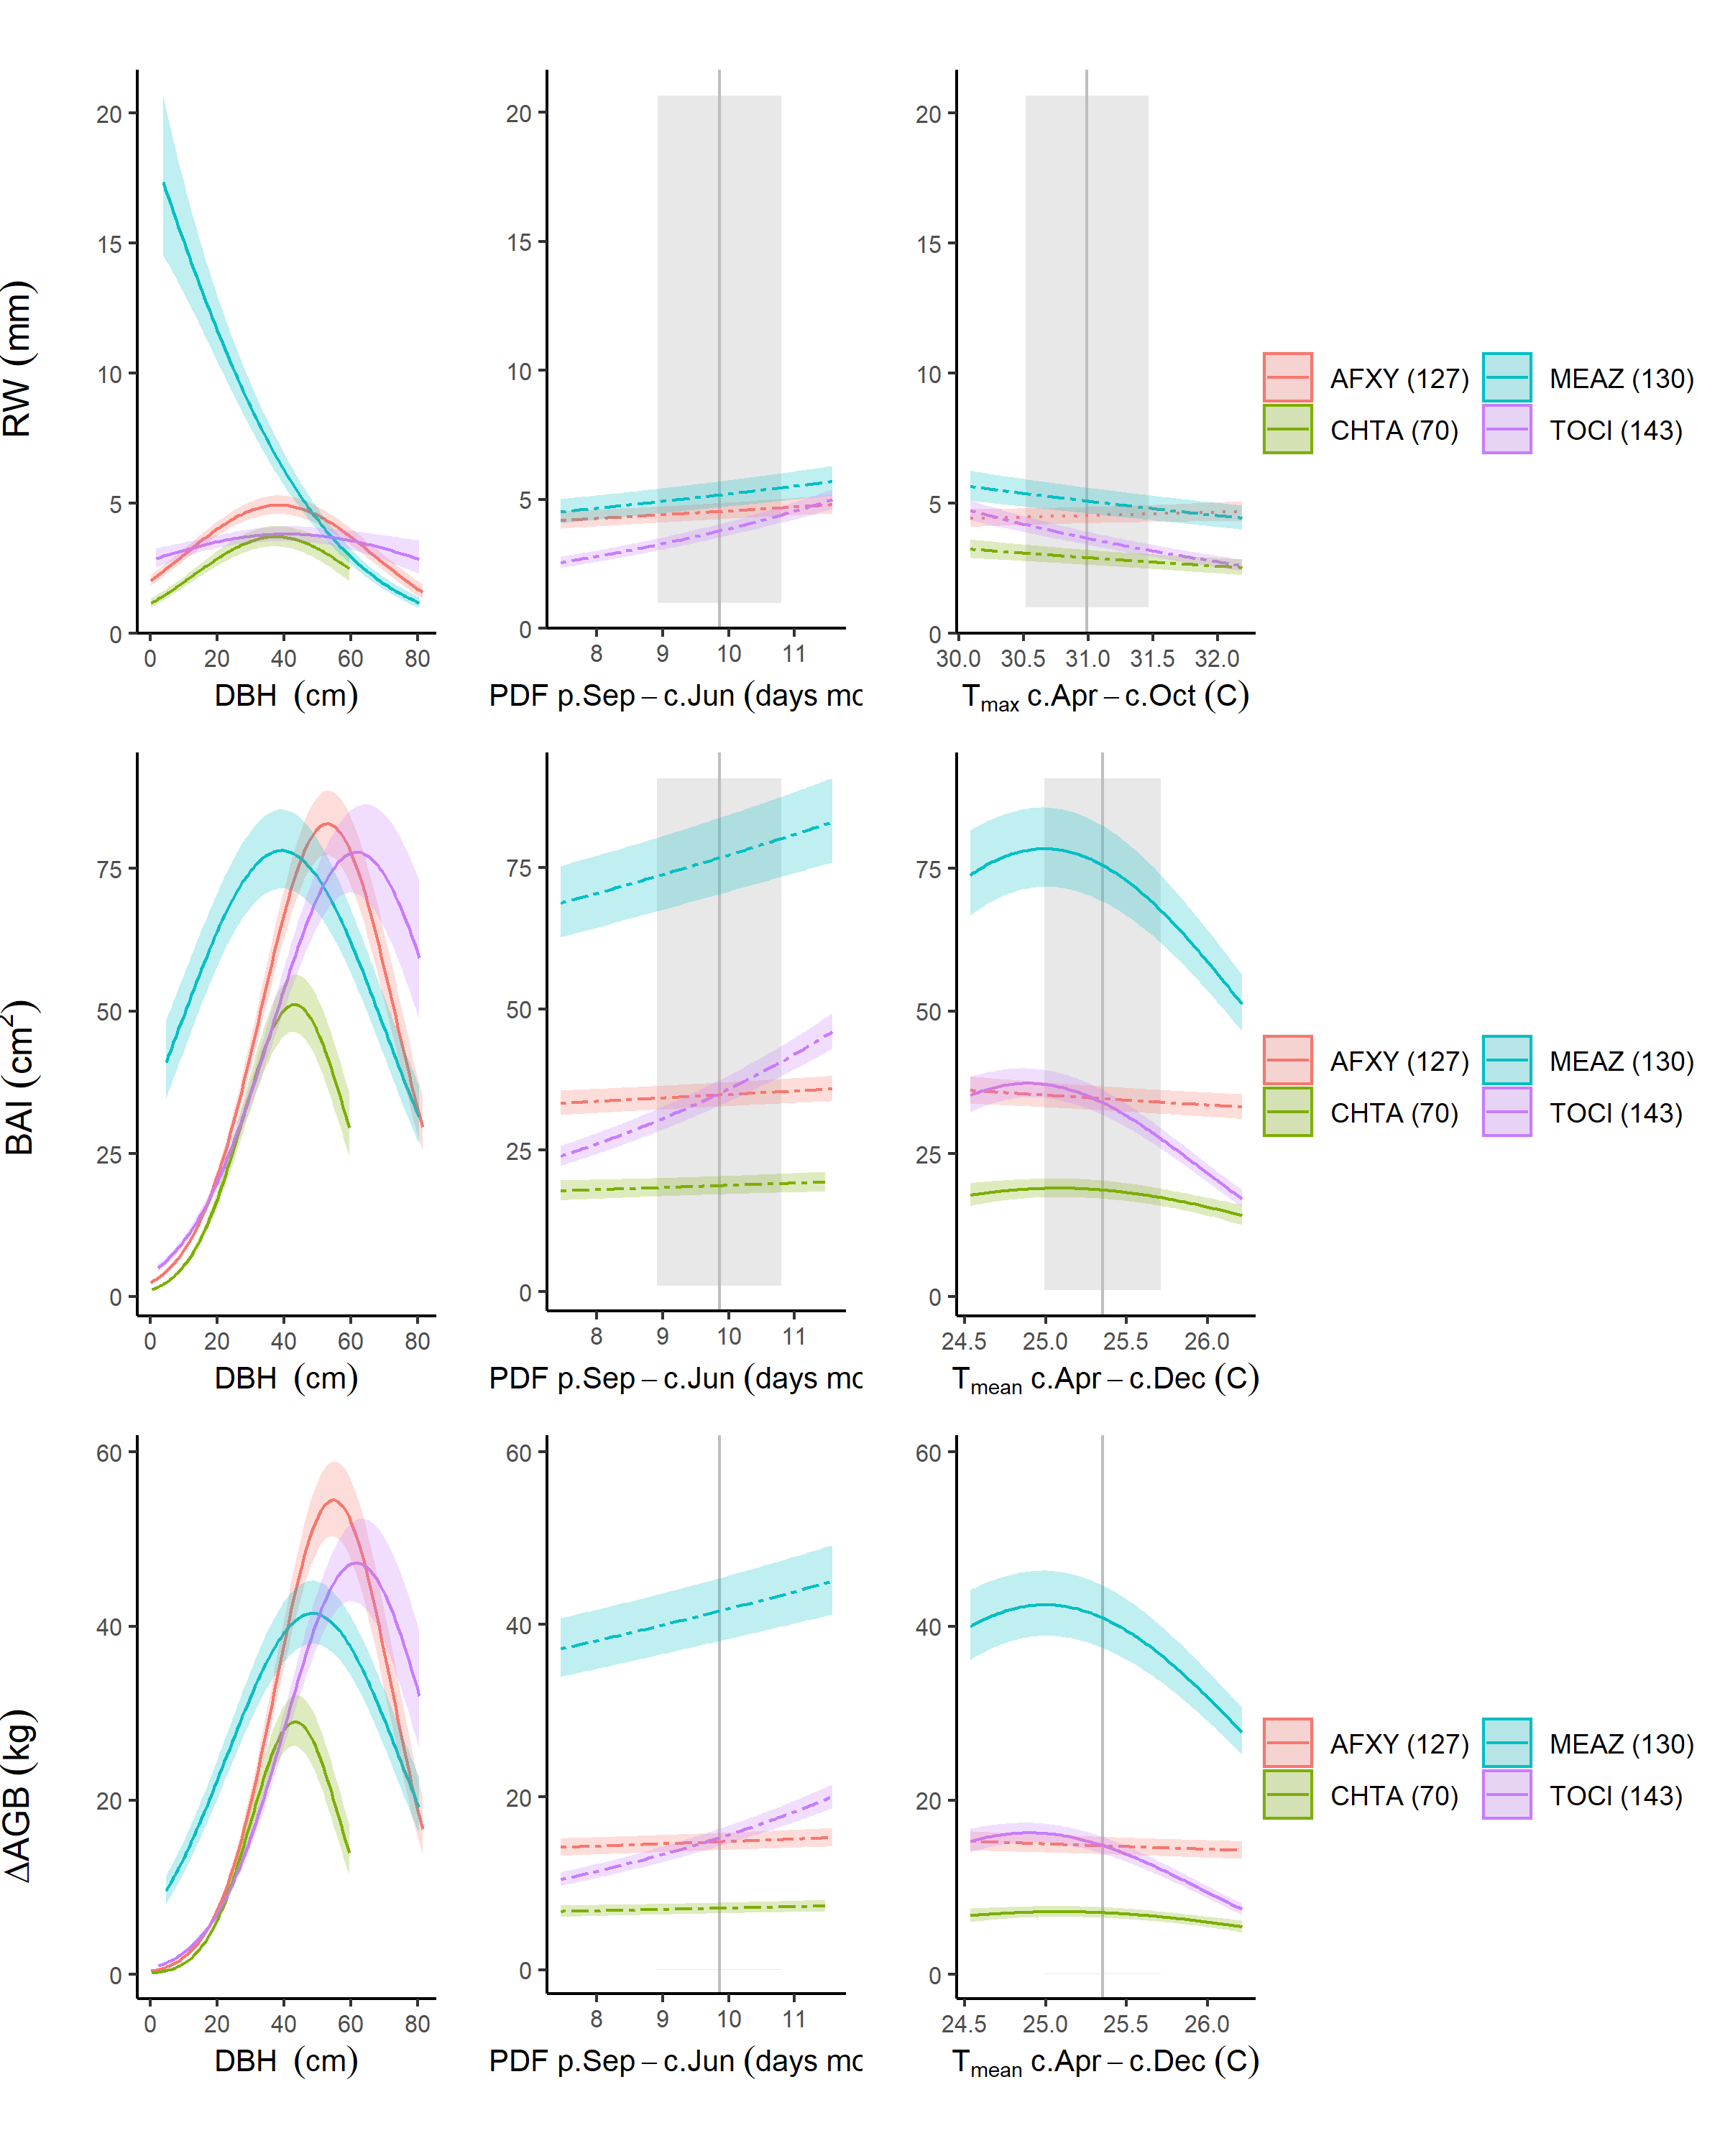
\includegraphics[width=0.75\textwidth,height=\textheight]{tables_figures/SI_figures/composite_plots/HKK.png}
\caption{Figure S10. Best GLS models for Huai Kha Khaeng (Thailand) for
all three growth metrics examined here. Precipitation and temperature
group variables are as selected by \emph{climwin} (p=previous year,
c=current year). For each species, relationships are plotted if included
in top model, with best-fit polynomials plotted with solid lines when
both first- and second-order terms are signficant, dashed lines when
only one term is signficant, and dotted lines when neither is
signficant. Transparent ribbons indicate 95\% confidence intervals.
Vertical grey lines indicate the long-term mean for the climate
variable, shading indicates 1 SD.}
\end{figure}

\newpage

\hypertarget{figure-s11.-best-gls-models-for-the-smithsonian-conservation-biology-institute-virginia-usa}{%
\subsection{Figure S11. Best GLS models for the Smithsonian Conservation
Biology Institute (Virginia,
USA)}\label{figure-s11.-best-gls-models-for-the-smithsonian-conservation-biology-institute-virginia-usa}}

\begin{figure}
\centering
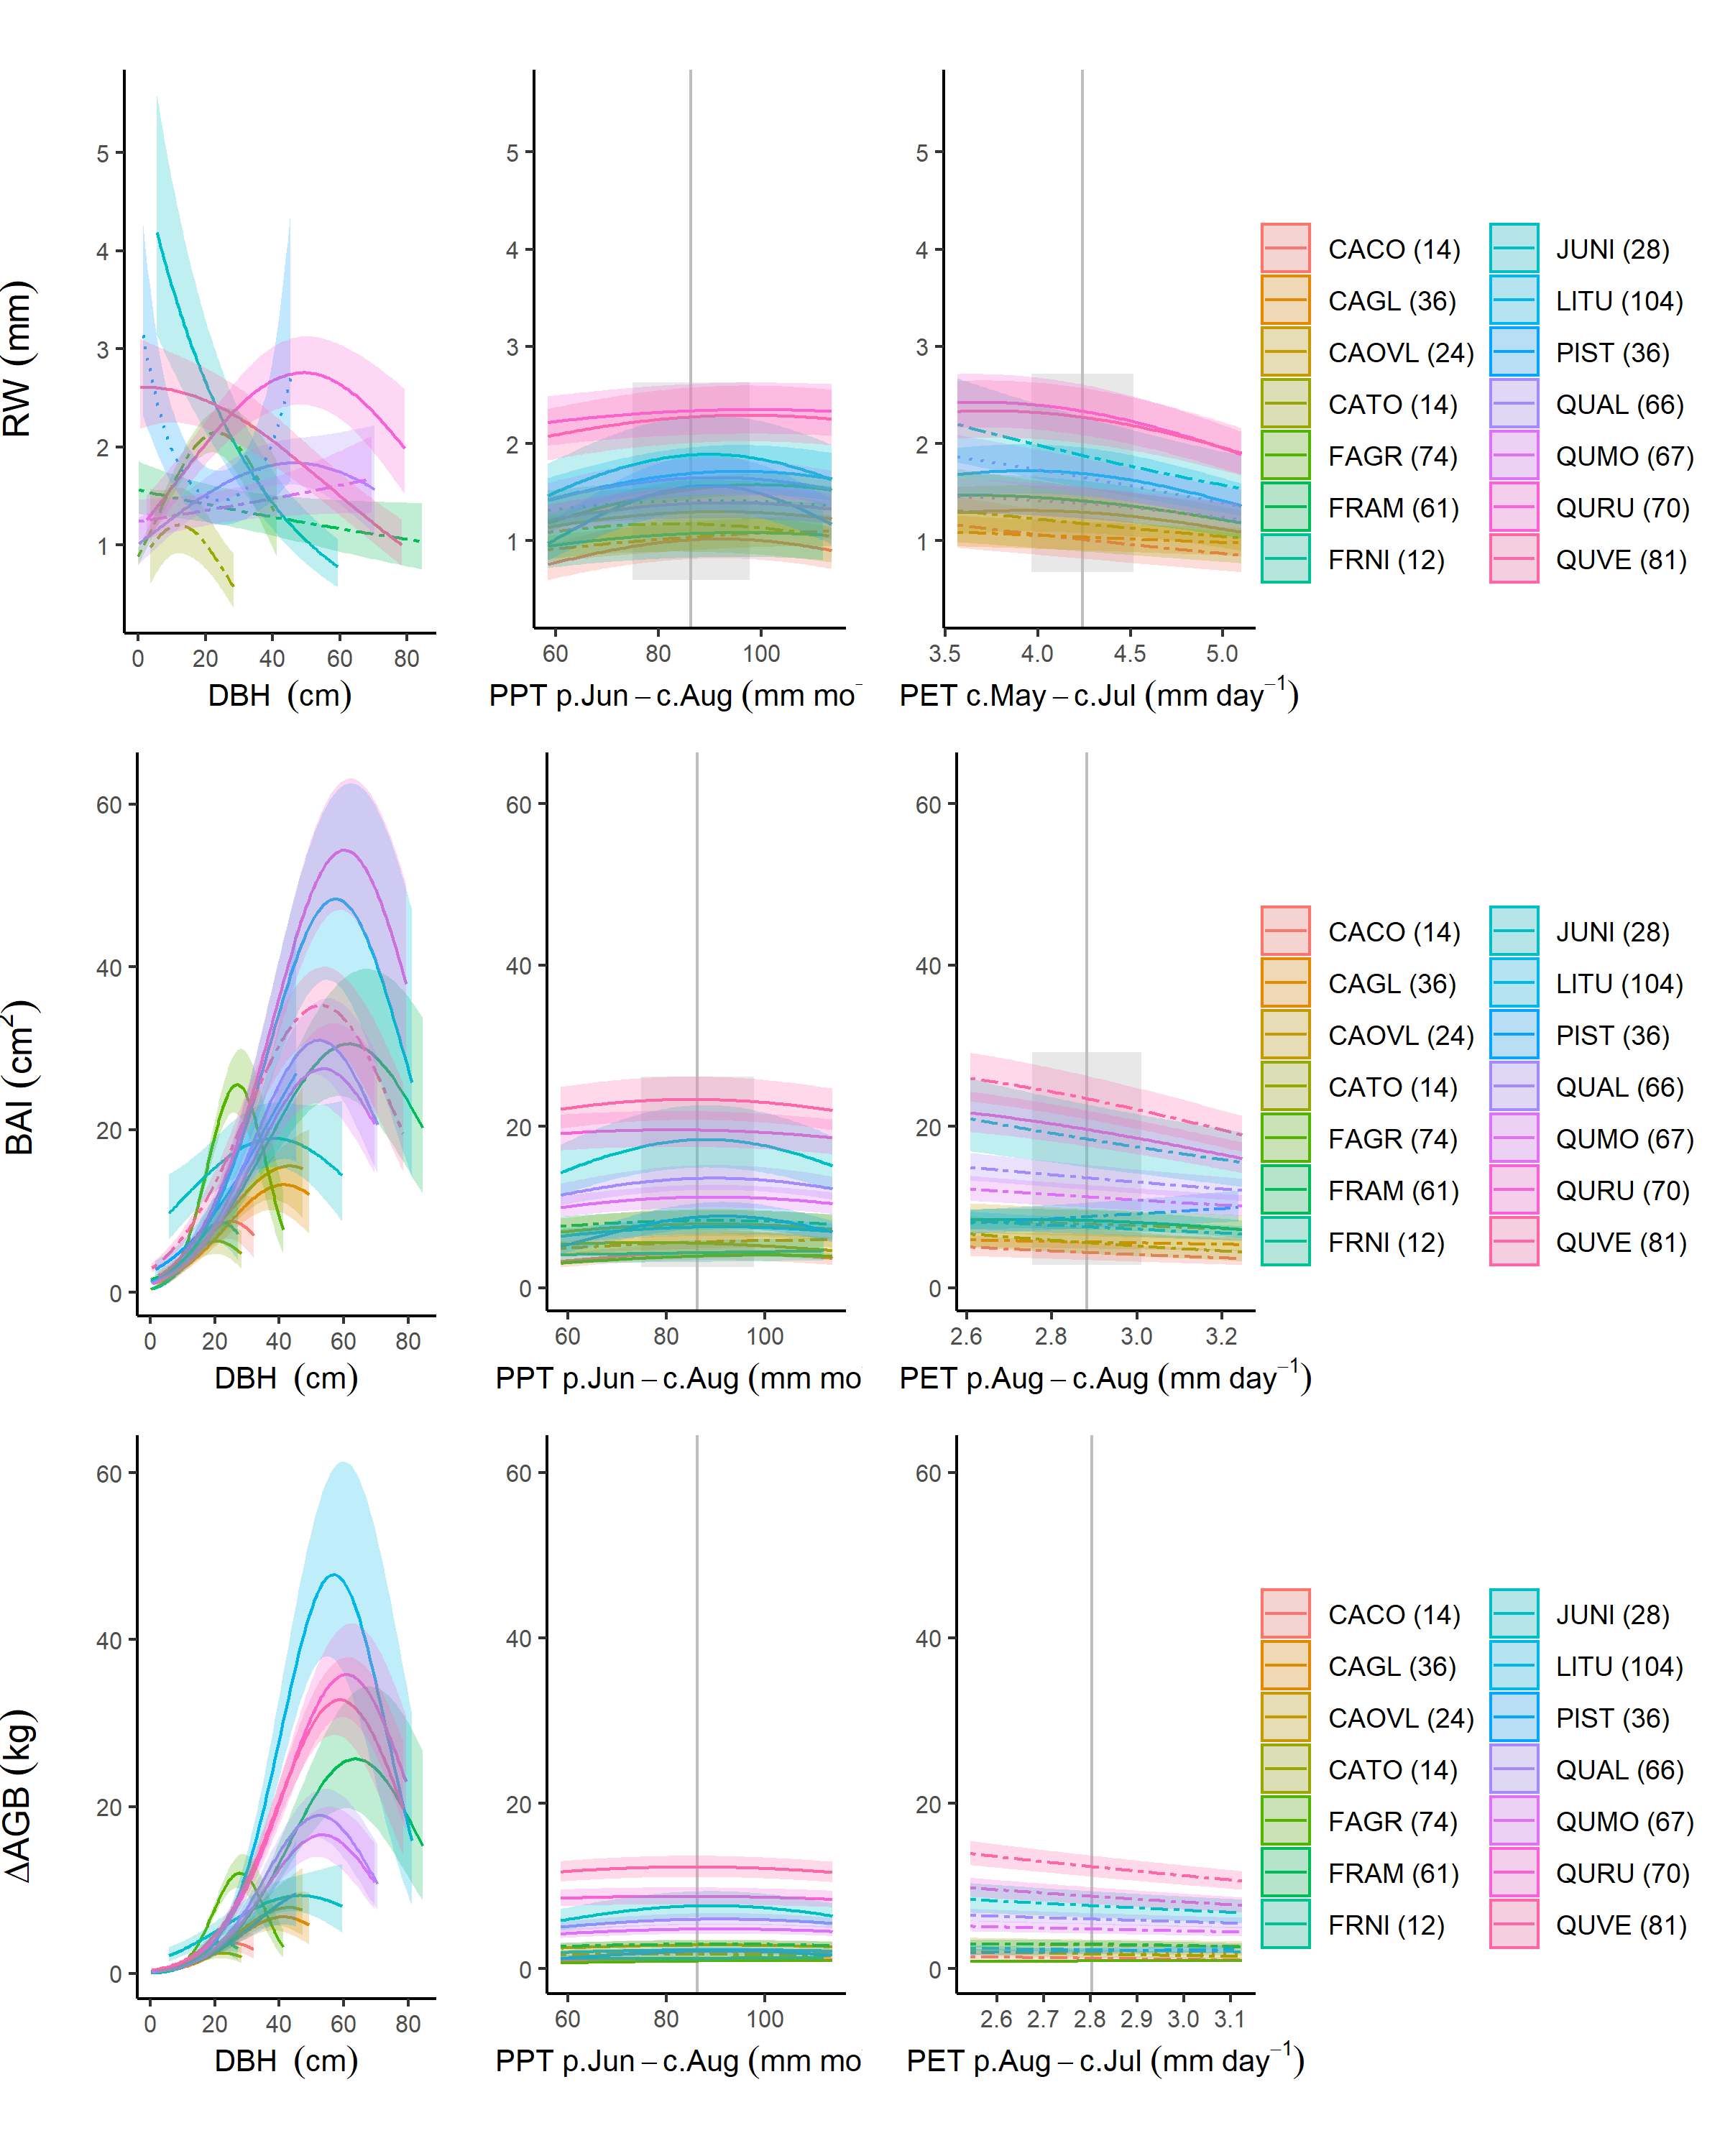
\includegraphics[width=0.75\textwidth,height=\textheight]{tables_figures/SI_figures/composite_plots/SCBI.png}
\caption{Figure S11. Best GLS models for the Smithsonian Conservation
Biology Institute (Virginia, USA) for all three growth metrics examined
here. Precipitation and temperature group variables are as selected by
\emph{climwin} (p=previous year, c=current year). For each species,
relationships are plotted if included in top model, with best-fit
polynomials plotted with solid lines when both first- and second-order
terms are signficant, dashed lines when only one term is signficant, and
dotted lines when neither is signficant. Transparent ribbons indicate
95\% confidence intervals. Vertical grey lines indicate the long-term
mean for the climate variable, shading indicates 1 SD.}
\end{figure}

\newpage

\hypertarget{figure-s12.-best-gls-models-for-lilley-dickey-woods-indiana-usa}{%
\subsection{Figure S12. Best GLS models for Lilley Dickey Woods
(Indiana,
USA)}\label{figure-s12.-best-gls-models-for-lilley-dickey-woods-indiana-usa}}

\begin{figure}
\centering
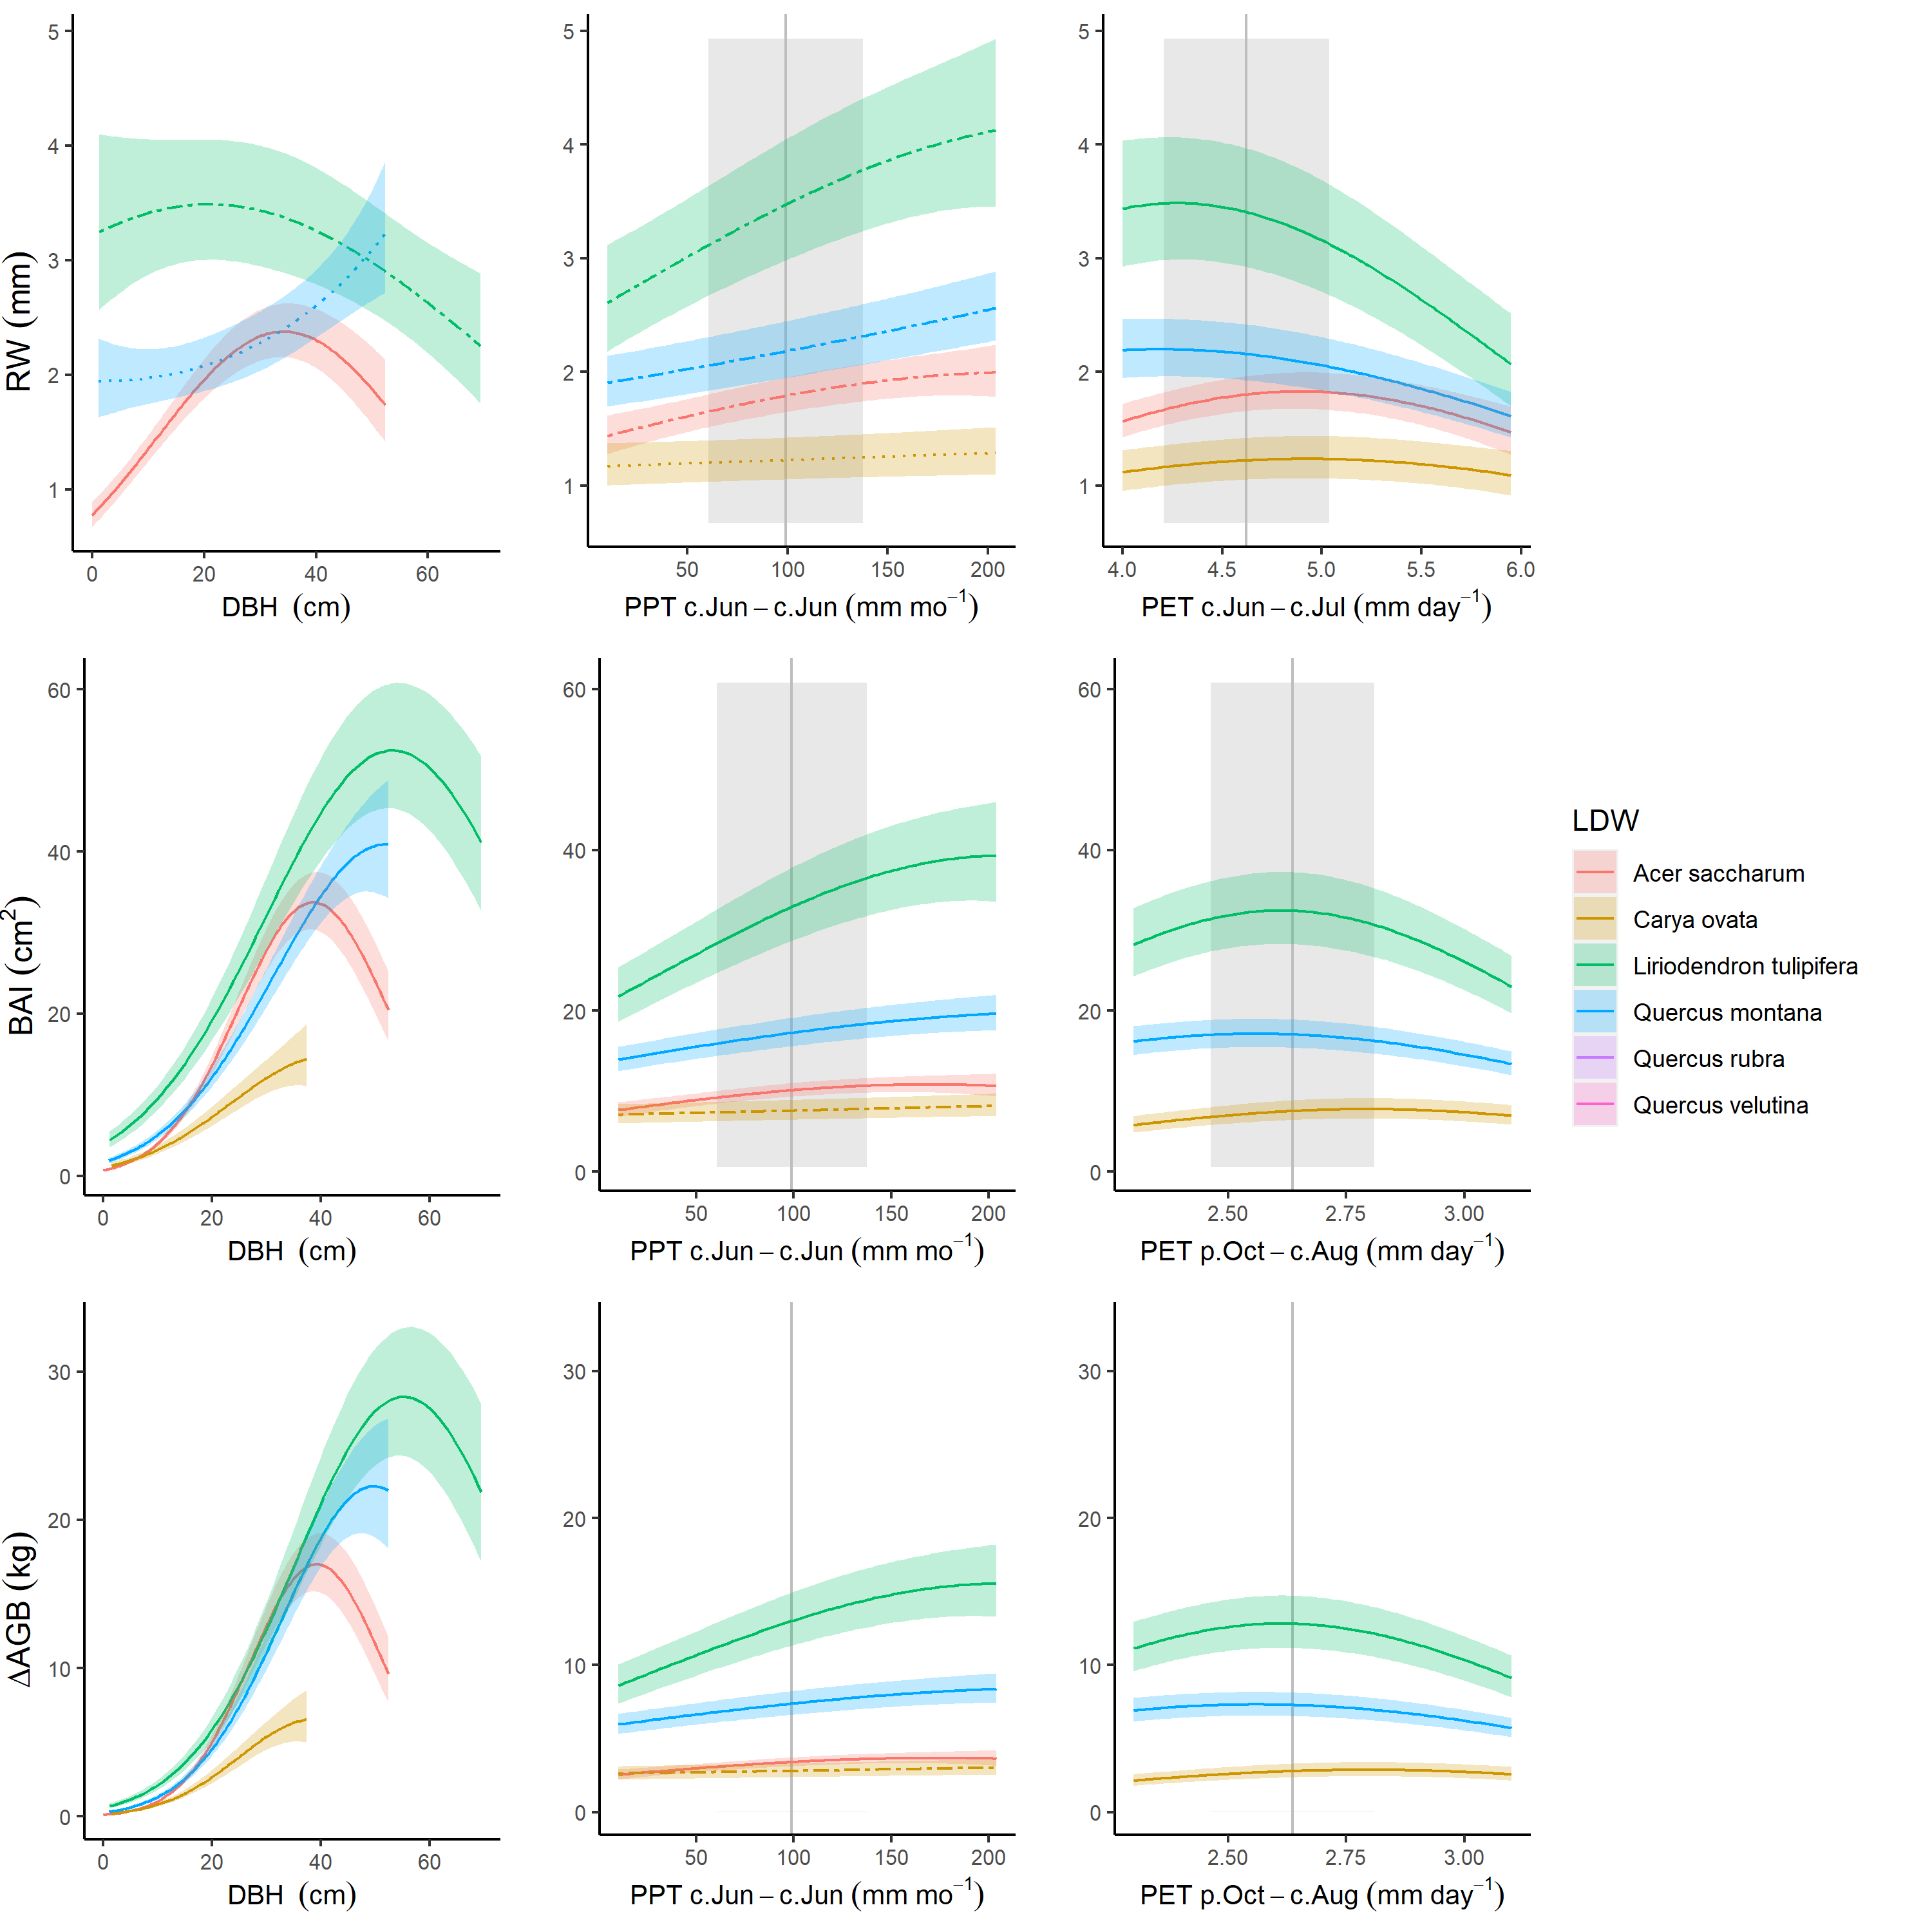
\includegraphics[width=0.75\textwidth,height=\textheight]{tables_figures/SI_figures/composite_plots/LillyDickey.png}
\caption{Figure S12. Best GLS models for Lilley Dickey Woods (Indiana,
USA) for all three growth metrics examined here. Precipitation and
temperature group variables are as selected by \emph{climwin}
(p=previous year, c=current year). For each species, relationships are
plotted if included in top model, with best-fit polynomials plotted with
solid lines when both first- and second-order terms are signficant,
dashed lines when only one term is signficant, and dotted lines when
neither is signficant. Transparent ribbons indicate 95\% confidence
intervals. Vertical grey lines indicate the long-term mean for the
climate variable, shading indicates 1 SD.}
\end{figure}

\newpage

\hypertarget{figure-s13.-best-gls-models-for-harvard-forest-massachusetts-usa}{%
\subsection{Figure S13. Best GLS models for Harvard Forest
(Massachusetts,
USA)}\label{figure-s13.-best-gls-models-for-harvard-forest-massachusetts-usa}}

\begin{figure}
\centering
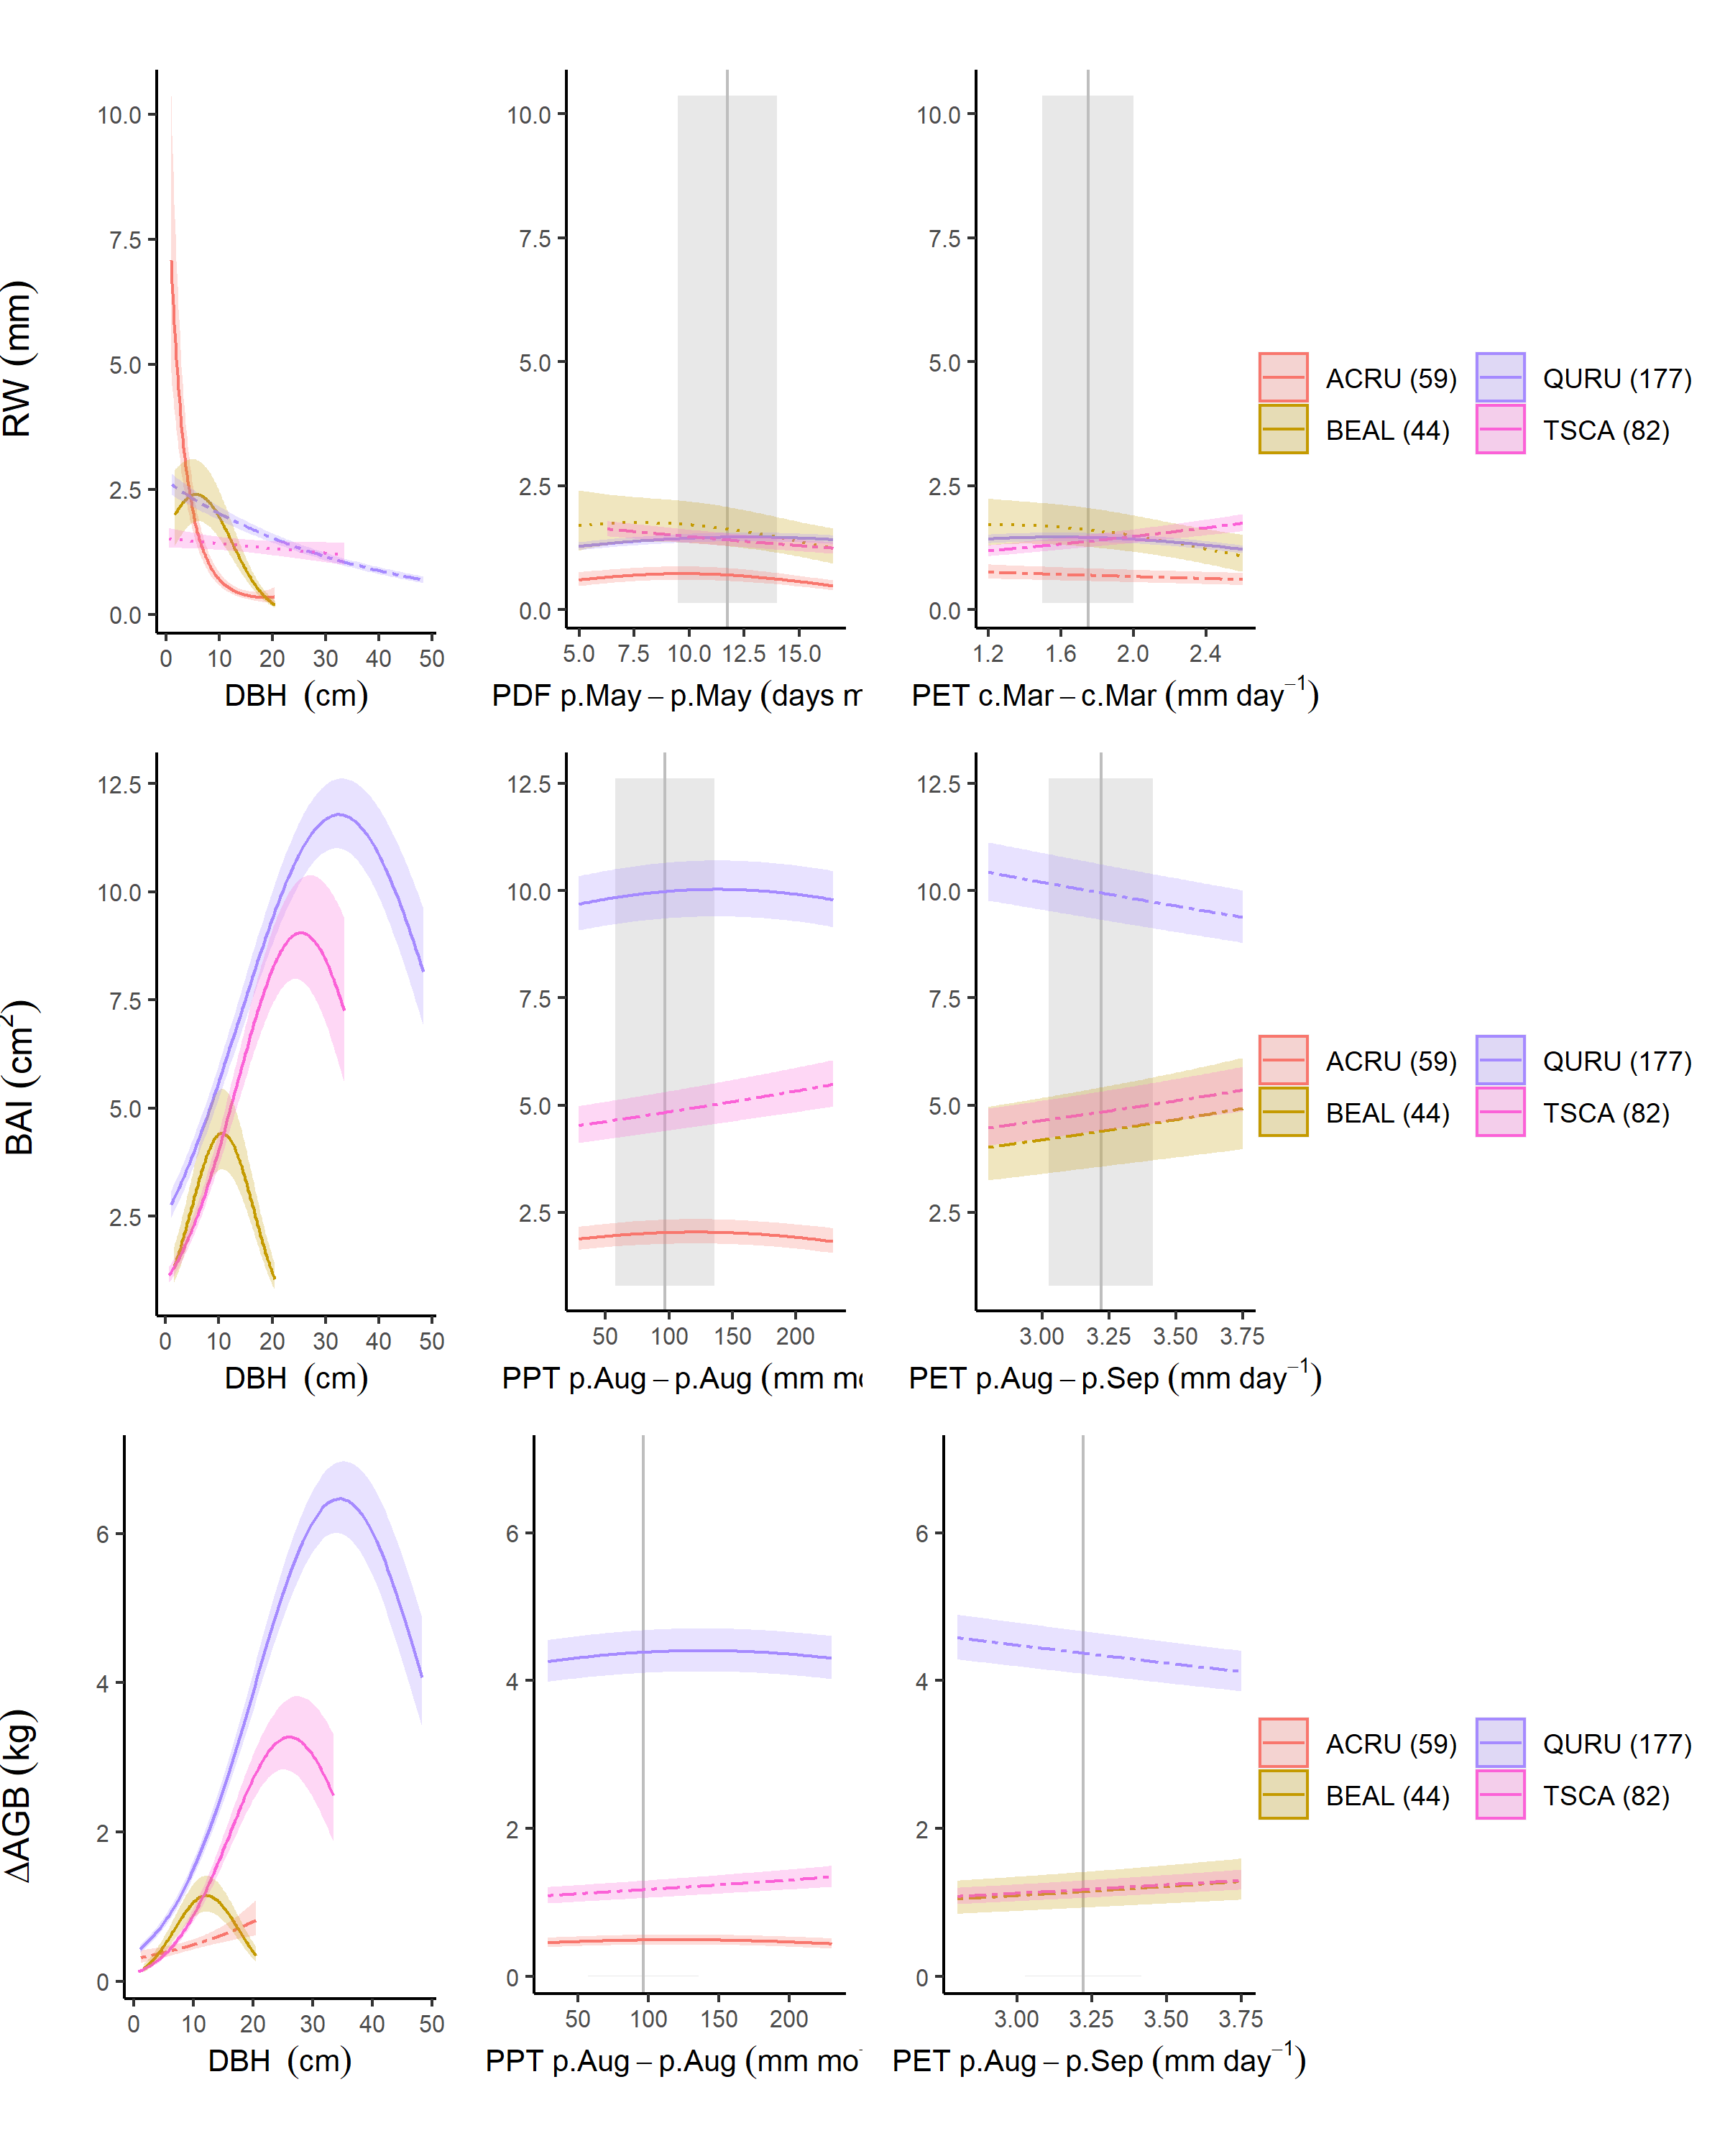
\includegraphics[width=0.75\textwidth,height=\textheight]{tables_figures/SI_figures/composite_plots/HarvardForest.png}
\caption{Figure S13. Best GLS models for Harvard Forest (Massachusetts,
USA) for all three growth metrics examined here. Precipitation and
temperature group variables are as selected by \emph{climwin}
(p=previous year, c=current year). For each species, relationships are
plotted if included in top model, with best-fit polynomials plotted with
solid lines when both first- and second-order terms are signficant,
dashed lines when only one term is signficant, and dotted lines when
neither is signficant. Transparent ribbons indicate 95\% confidence
intervals. Vertical grey lines indicate the long-term mean for the
climate variable, shading indicates 1 SD.}
\end{figure}

\newpage

\hypertarget{figure-s14.-best-gls-models-for-zofin-forest-czech-republic}{%
\subsection{Figure S14. Best GLS models for Zofin Forest (Czech
Republic)}\label{figure-s14.-best-gls-models-for-zofin-forest-czech-republic}}

\begin{figure}
\centering
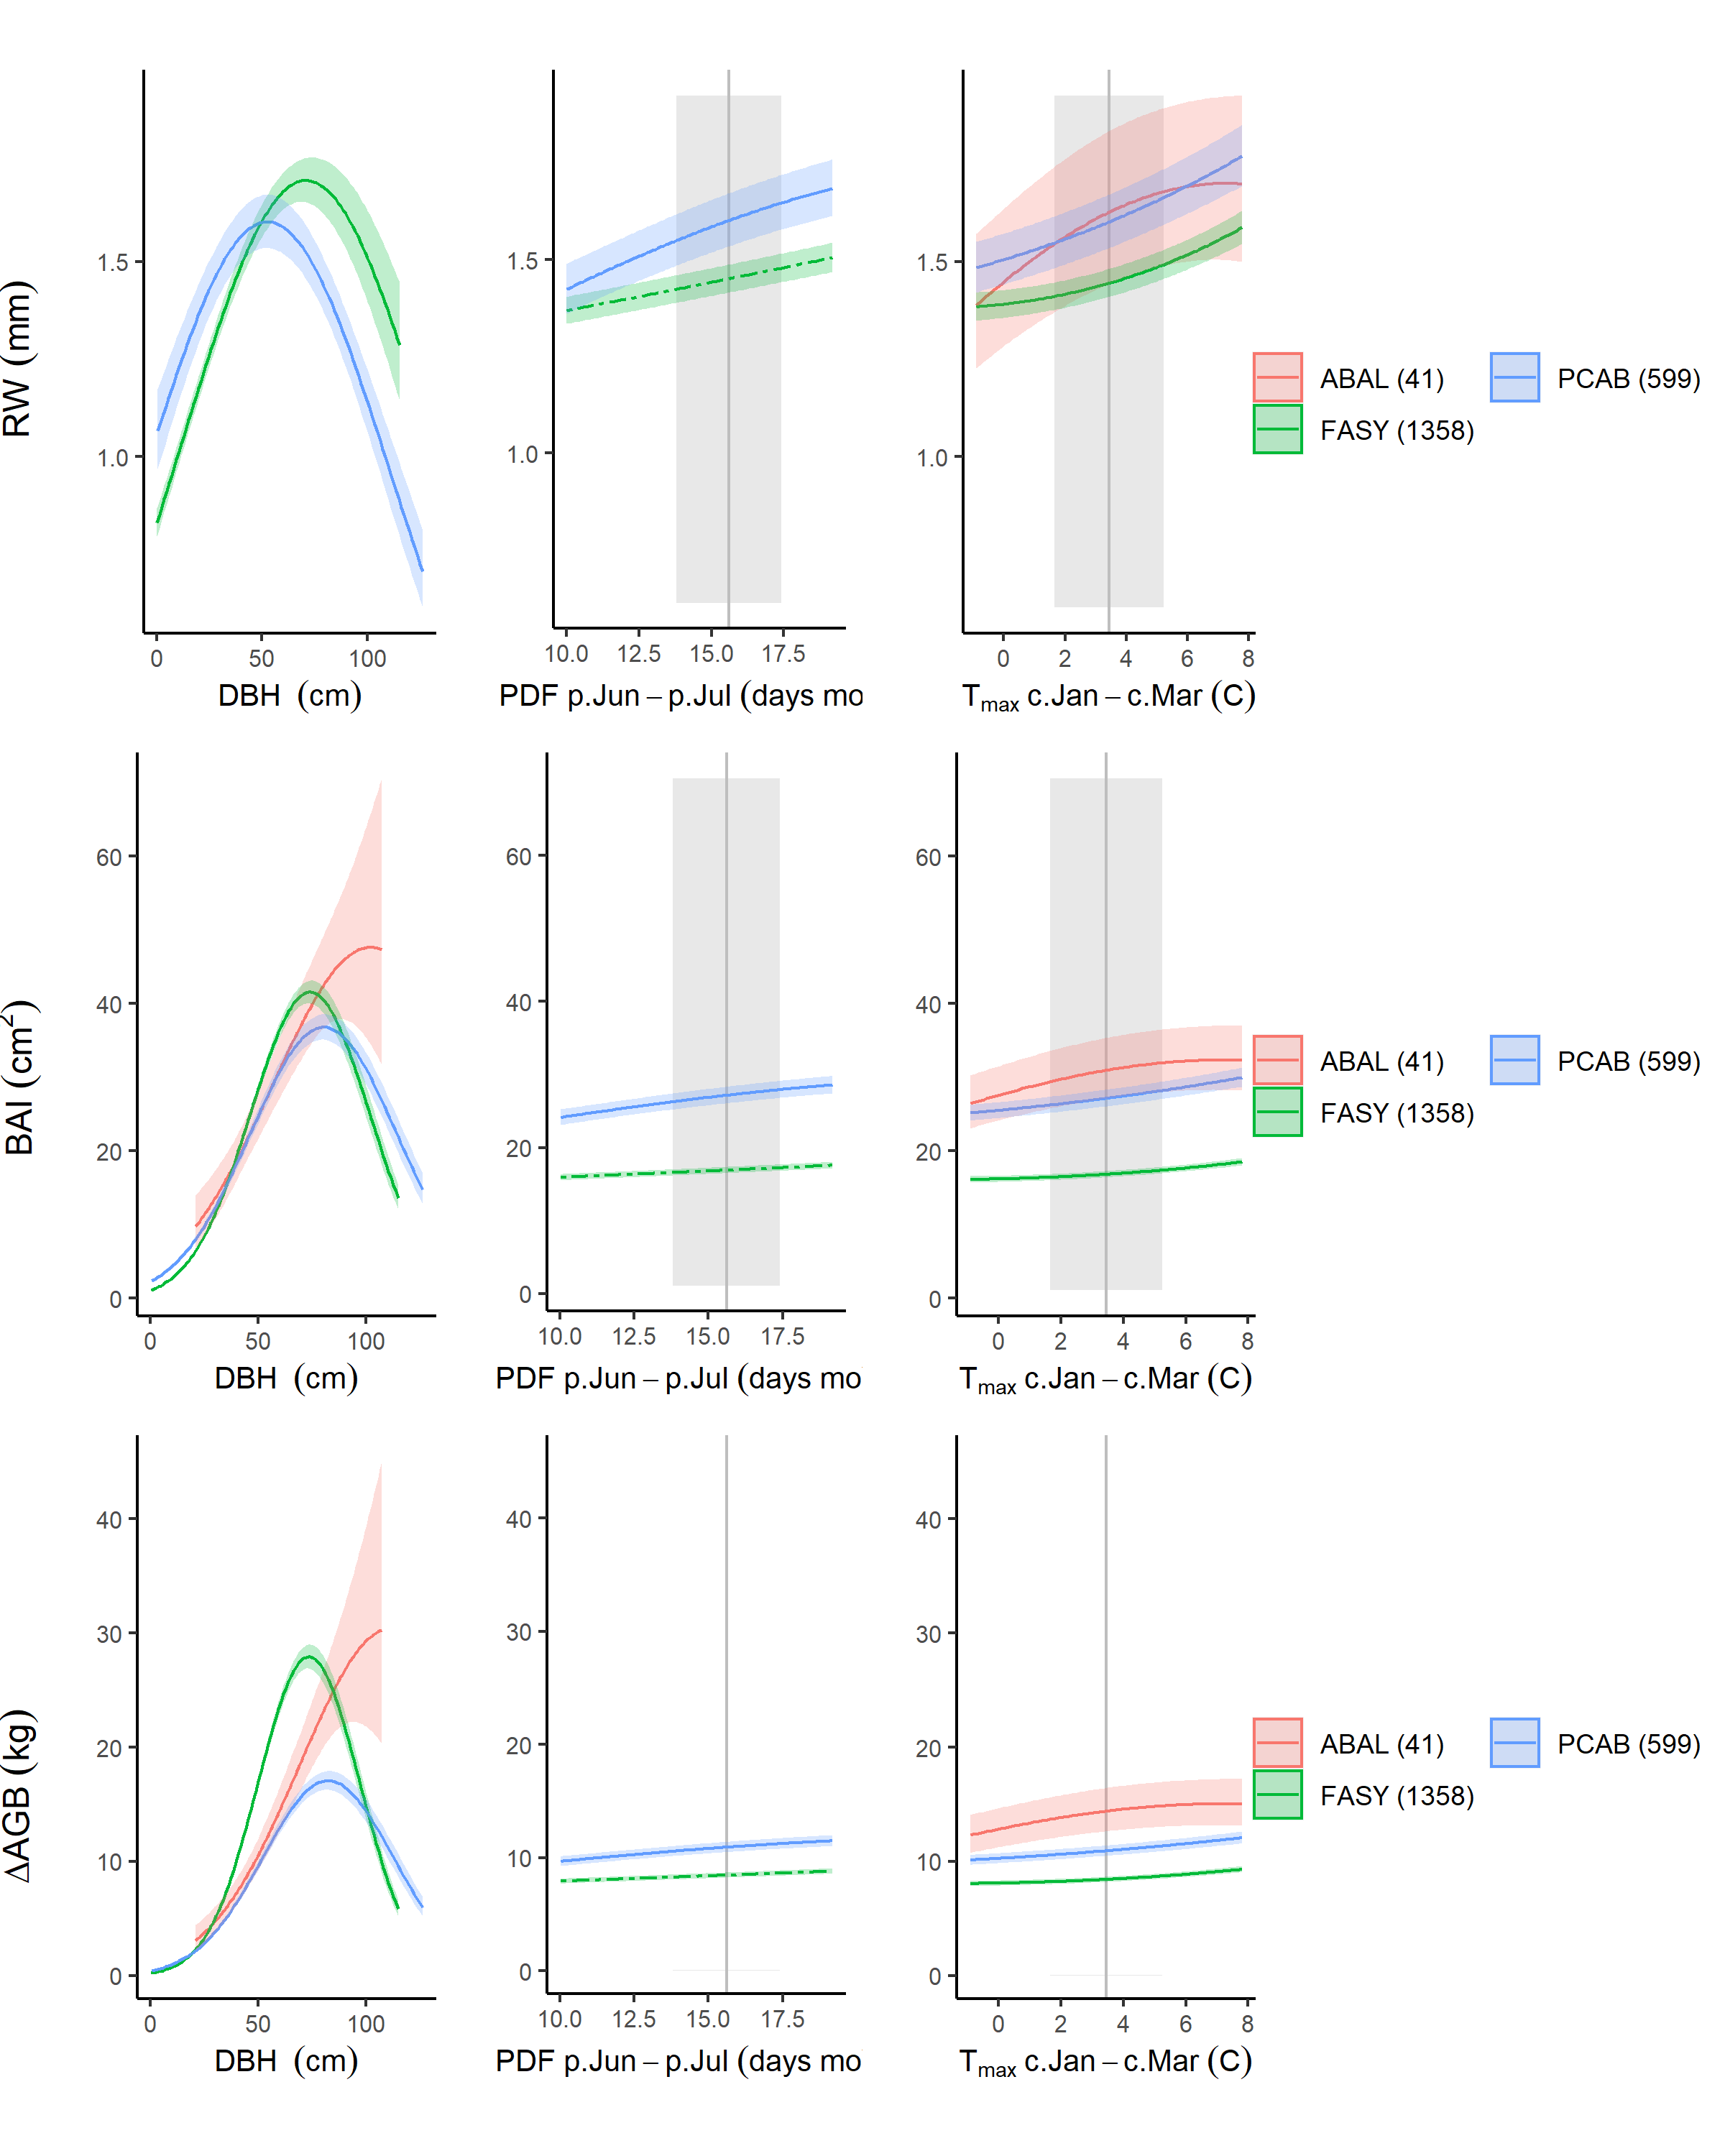
\includegraphics[width=0.75\textwidth,height=\textheight]{tables_figures/SI_figures/composite_plots/Zofin.png}
\caption{Figure S14. Best GLS models for Zofin Forest (Czech Republic)
for all three growth metrics examined here. Precipitation and
temperature group variables are as selected by \emph{climwin}
(p=previous year, c=current year). For each species, relationships are
plotted if included in top model, with best-fit polynomials plotted with
solid lines when both first- and second-order terms are signficant,
dashed lines when only one term is signficant, and dotted lines when
neither is signficant. Transparent ribbons indicate 95\% confidence
intervals. Vertical grey lines indicate the long-term mean for the
climate variable, shading indicates 1 SD.}
\end{figure}

\newpage

\hypertarget{figure-s15.-best-gls-models-for-niobrara-halsey-nebraska-usa}{%
\subsection{Figure S15. Best GLS models for Niobrara/ Halsey (Nebraska,
USA)}\label{figure-s15.-best-gls-models-for-niobrara-halsey-nebraska-usa}}

\begin{figure}
\centering
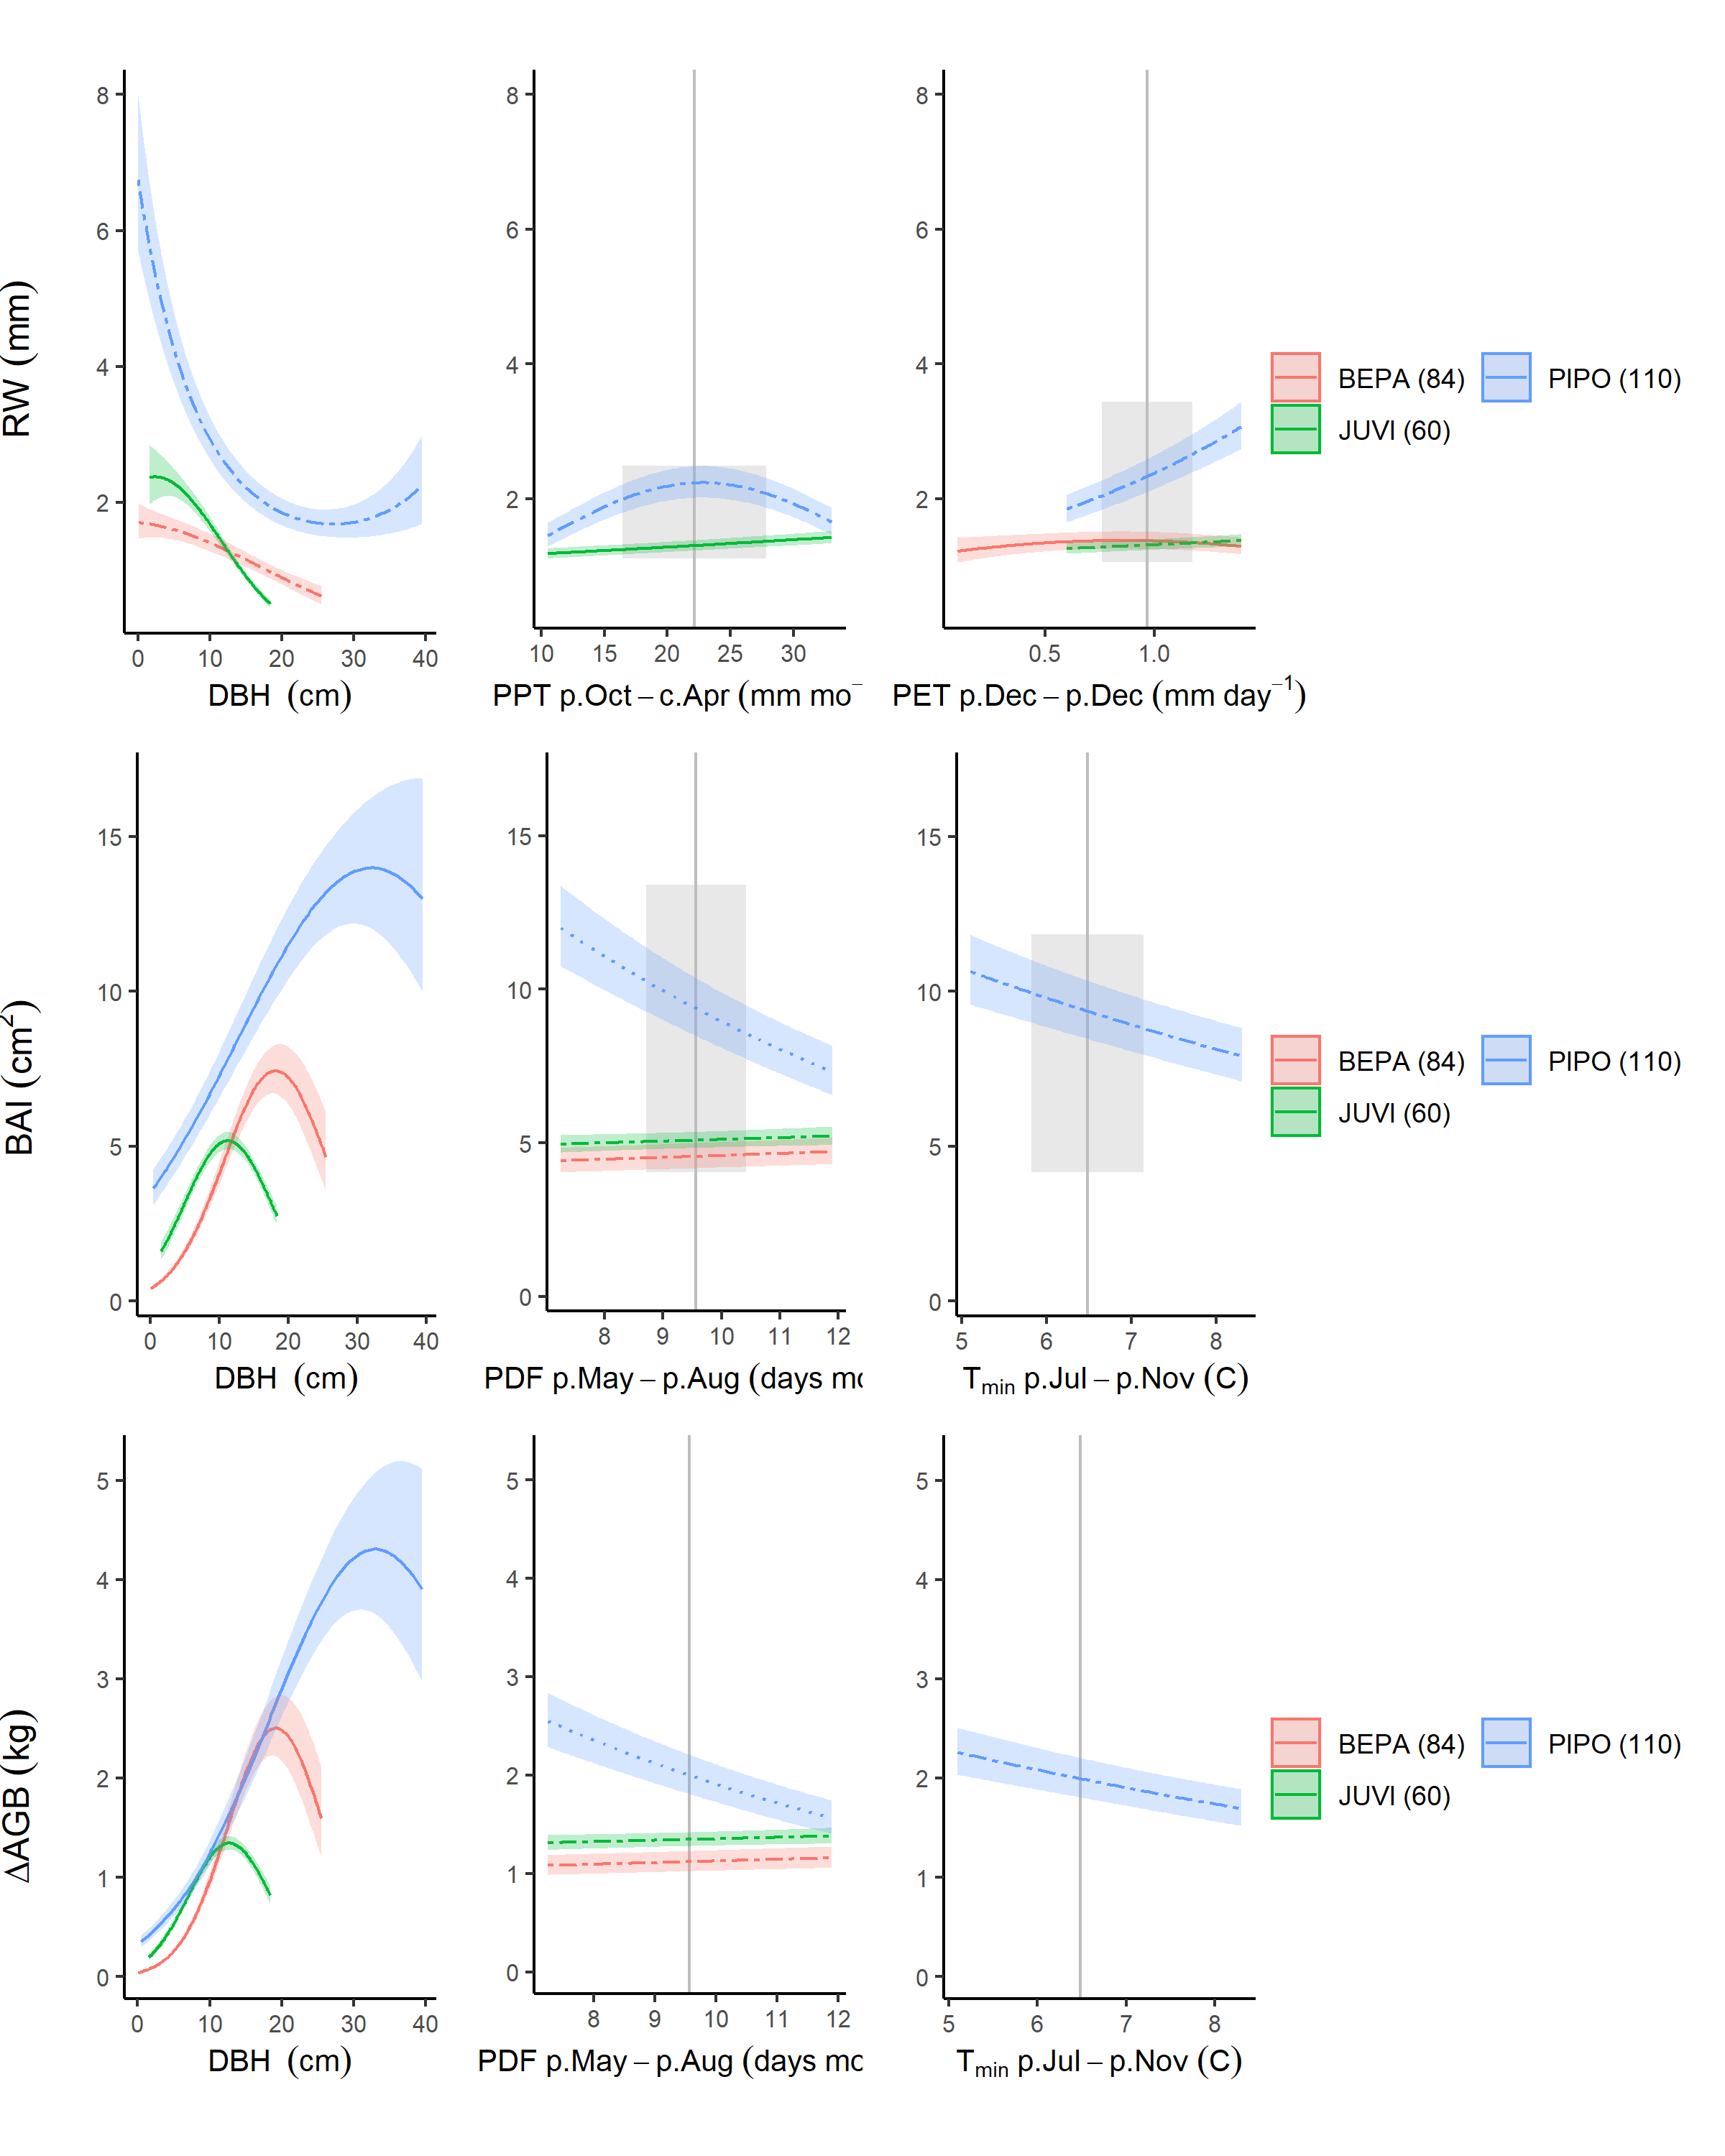
\includegraphics[width=0.75\textwidth,height=\textheight]{tables_figures/SI_figures/composite_plots/Nebraska.png}
\caption{Figure S15. Best GLS models for Niobrara/ Halsey (Nebraska,
USA) for all three growth metrics examined here. Precipitation and
temperature group variables are as selected by \emph{climwin}
(p=previous year, c=current year). For each species, relationships are
plotted if included in top model, with best-fit polynomials plotted with
solid lines when both first- and second-order terms are signficant,
dashed lines when only one term is signficant, and dotted lines when
neither is signficant. Transparent ribbons indicate 95\% confidence
intervals. Vertical grey lines indicate the long-term mean for the
climate variable, shading indicates 1 SD.}
\end{figure}

\newpage

\hypertarget{figure-s16.-best-gls-models-for-little-tesuque-new-mexico-usa}{%
\subsection{Figure S16. Best GLS models for Little Tesuque (New Mexico,
USA)}\label{figure-s16.-best-gls-models-for-little-tesuque-new-mexico-usa}}

\begin{figure}
\centering
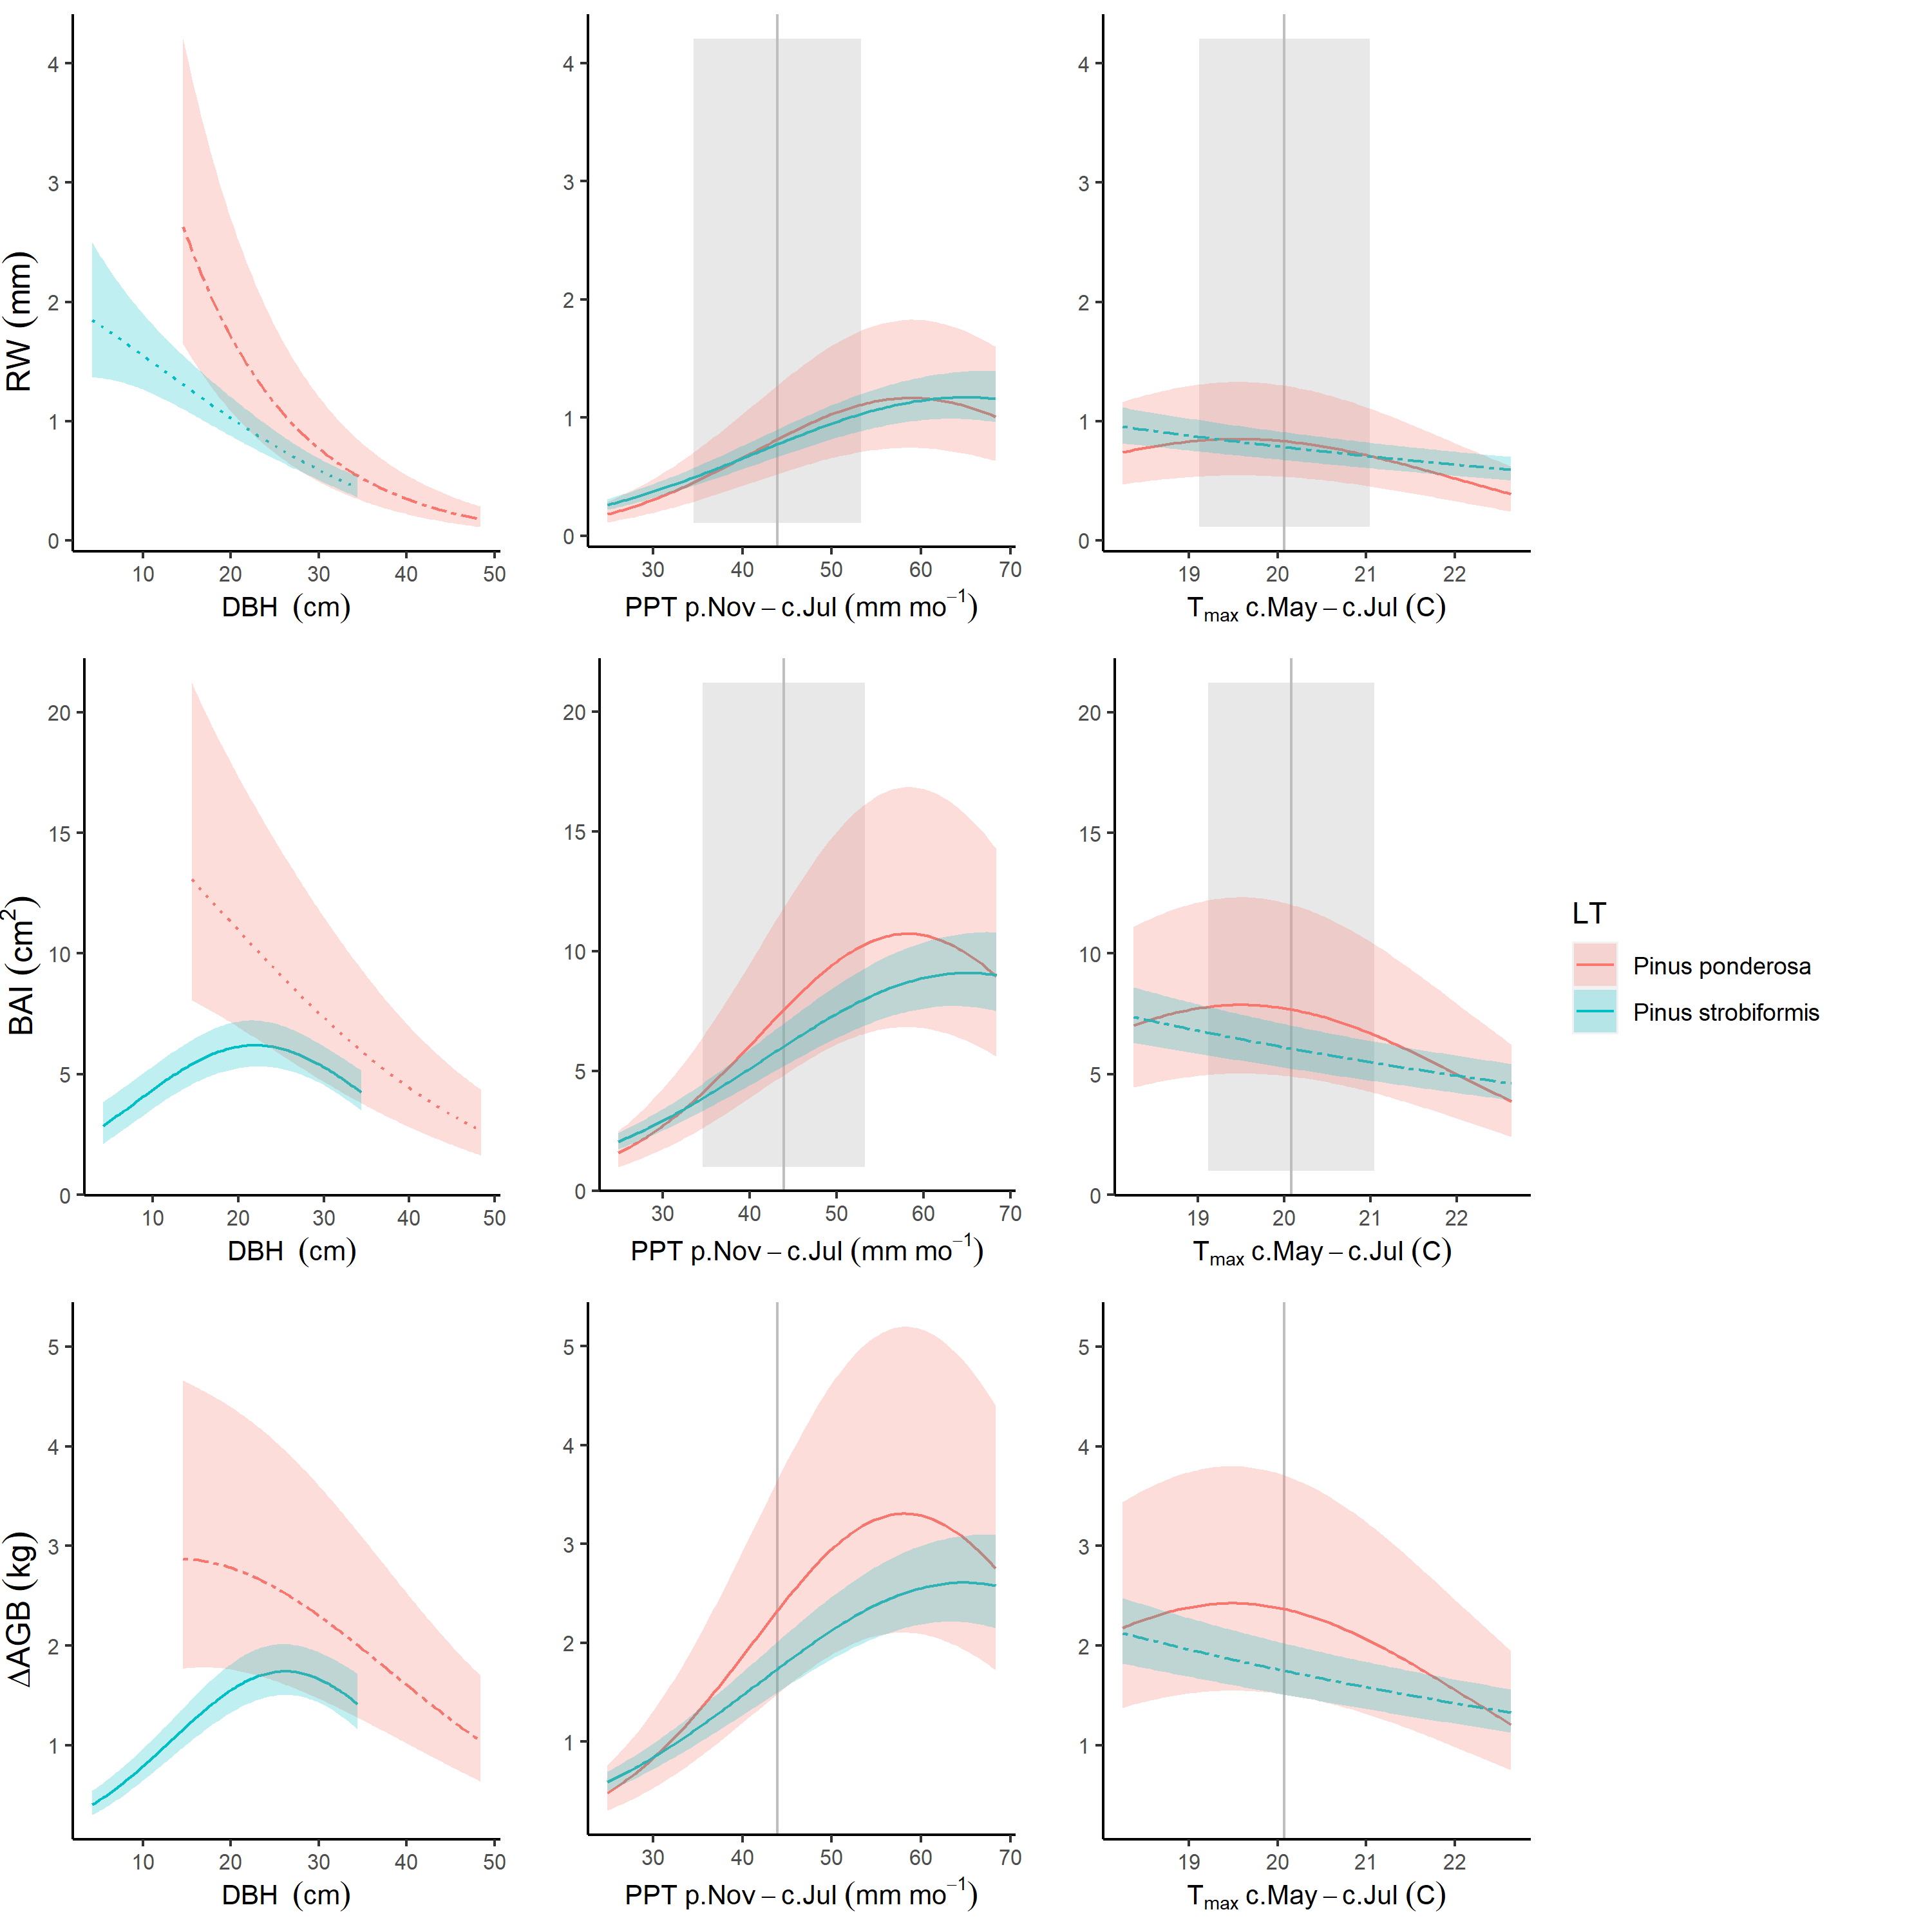
\includegraphics[width=0.75\textwidth,height=\textheight]{tables_figures/SI_figures/composite_plots/NewMexico.png}
\caption{Figure S16. Best GLS models for Little Tesuque (New Mexico,
USA) for all three growth metrics examined here. Precipitation and
temperature group variables are as selected by \emph{climwin}
(p=previous year, c=current year). For each species, relationships are
plotted if included in top model, with best-fit polynomials plotted with
solid lines when both first- and second-order terms are signficant,
dashed lines when only one term is signficant, and dotted lines when
neither is signficant. Transparent ribbons indicate 95\% confidence
intervals. Vertical grey lines indicate the long-term mean for the
climate variable, shading indicates 1 SD.}
\end{figure}

\newpage

\hypertarget{figure-s17.-best-gls-models-for-cedar-breaks-utah-usa}{%
\subsection{Figure S17. Best GLS models for Cedar Breaks (Utah,
USA)}\label{figure-s17.-best-gls-models-for-cedar-breaks-utah-usa}}

\begin{figure}
\centering
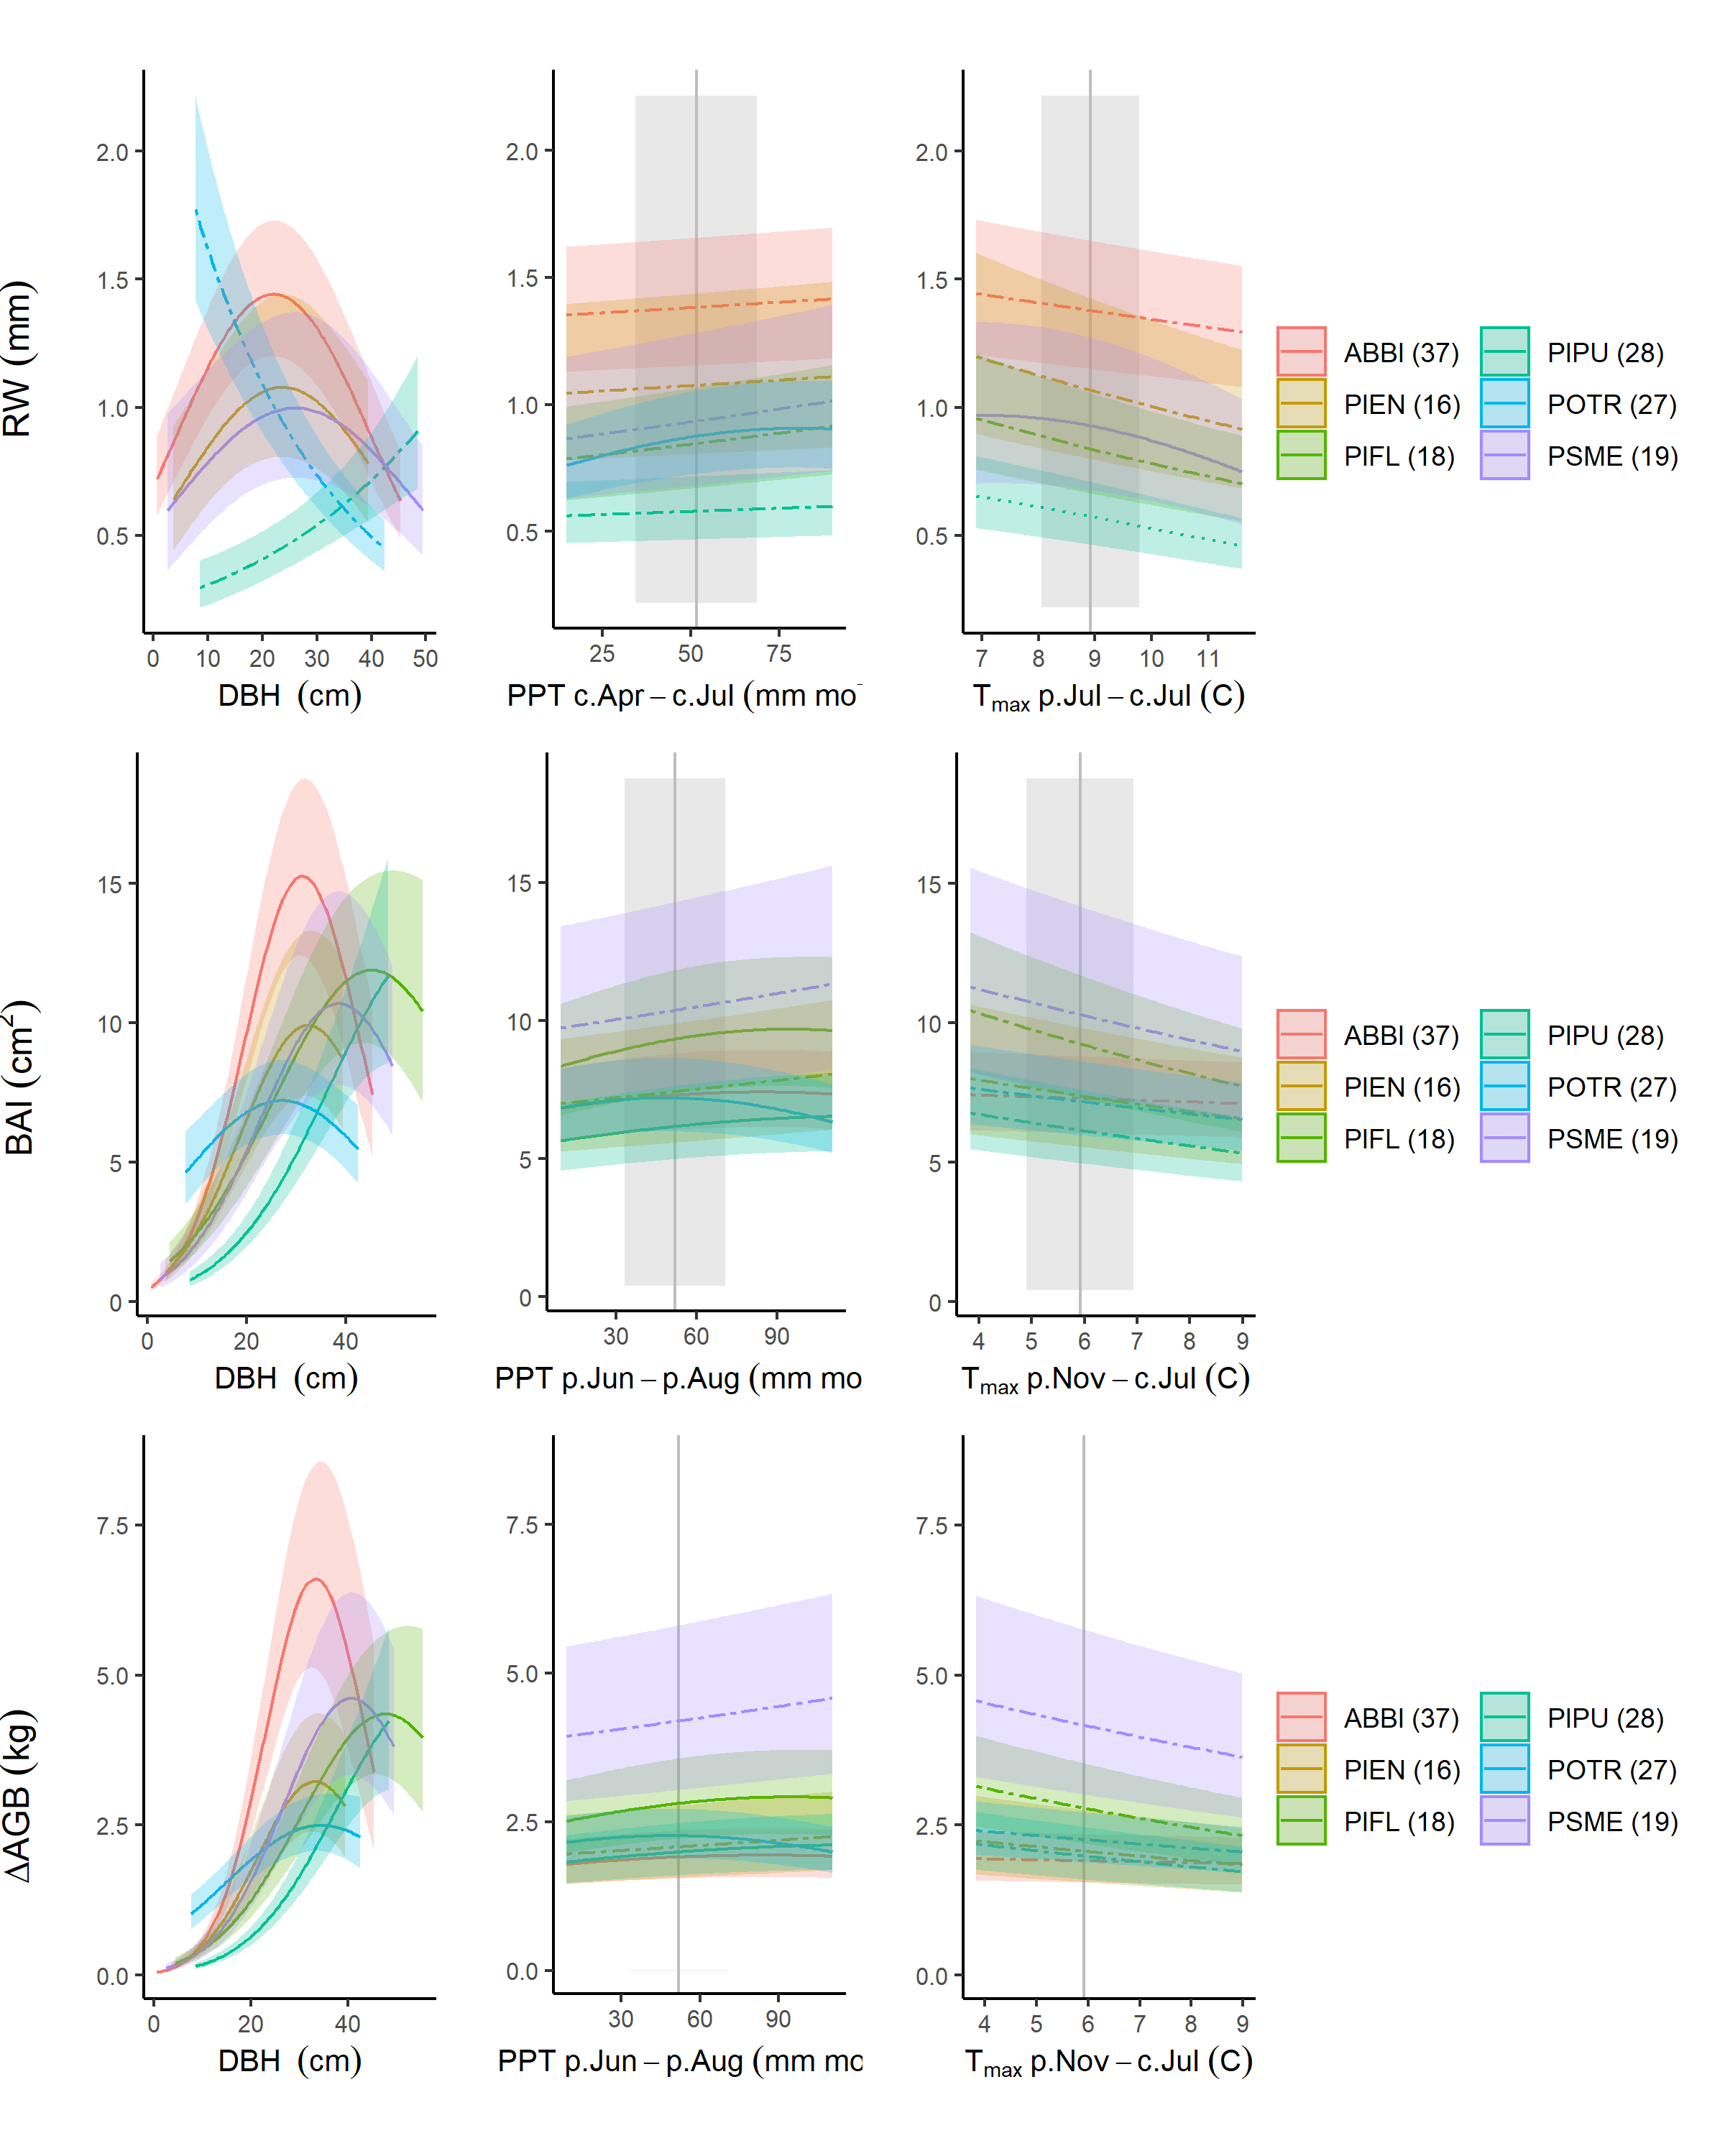
\includegraphics[width=0.75\textwidth,height=\textheight]{tables_figures/SI_figures/composite_plots/CedarBreaks.png}
\caption{Figure S17. Best GLS models for Cedar Breaks (Utah, USA) for
all three growth metrics examined here. Precipitation and temperature
group variables are as selected by \emph{climwin} (p=previous year,
c=current year). For each species, relationships are plotted if included
in top model, with best-fit polynomials plotted with solid lines when
both first- and second-order terms are signficant, dashed lines when
only one term is signficant, and dotted lines when neither is
signficant. Transparent ribbons indicate 95\% confidence intervals.
Vertical grey lines indicate the long-term mean for the climate
variable, shading indicates 1 SD.}
\end{figure}

\newpage

\hypertarget{figure-s18.-best-gls-models-for-scotty-creek-northwest-territory-canada}{%
\subsection{Figure S18. Best GLS models for Scotty Creek (Northwest
Territory,
Canada)}\label{figure-s18.-best-gls-models-for-scotty-creek-northwest-territory-canada}}

\begin{figure}
\centering
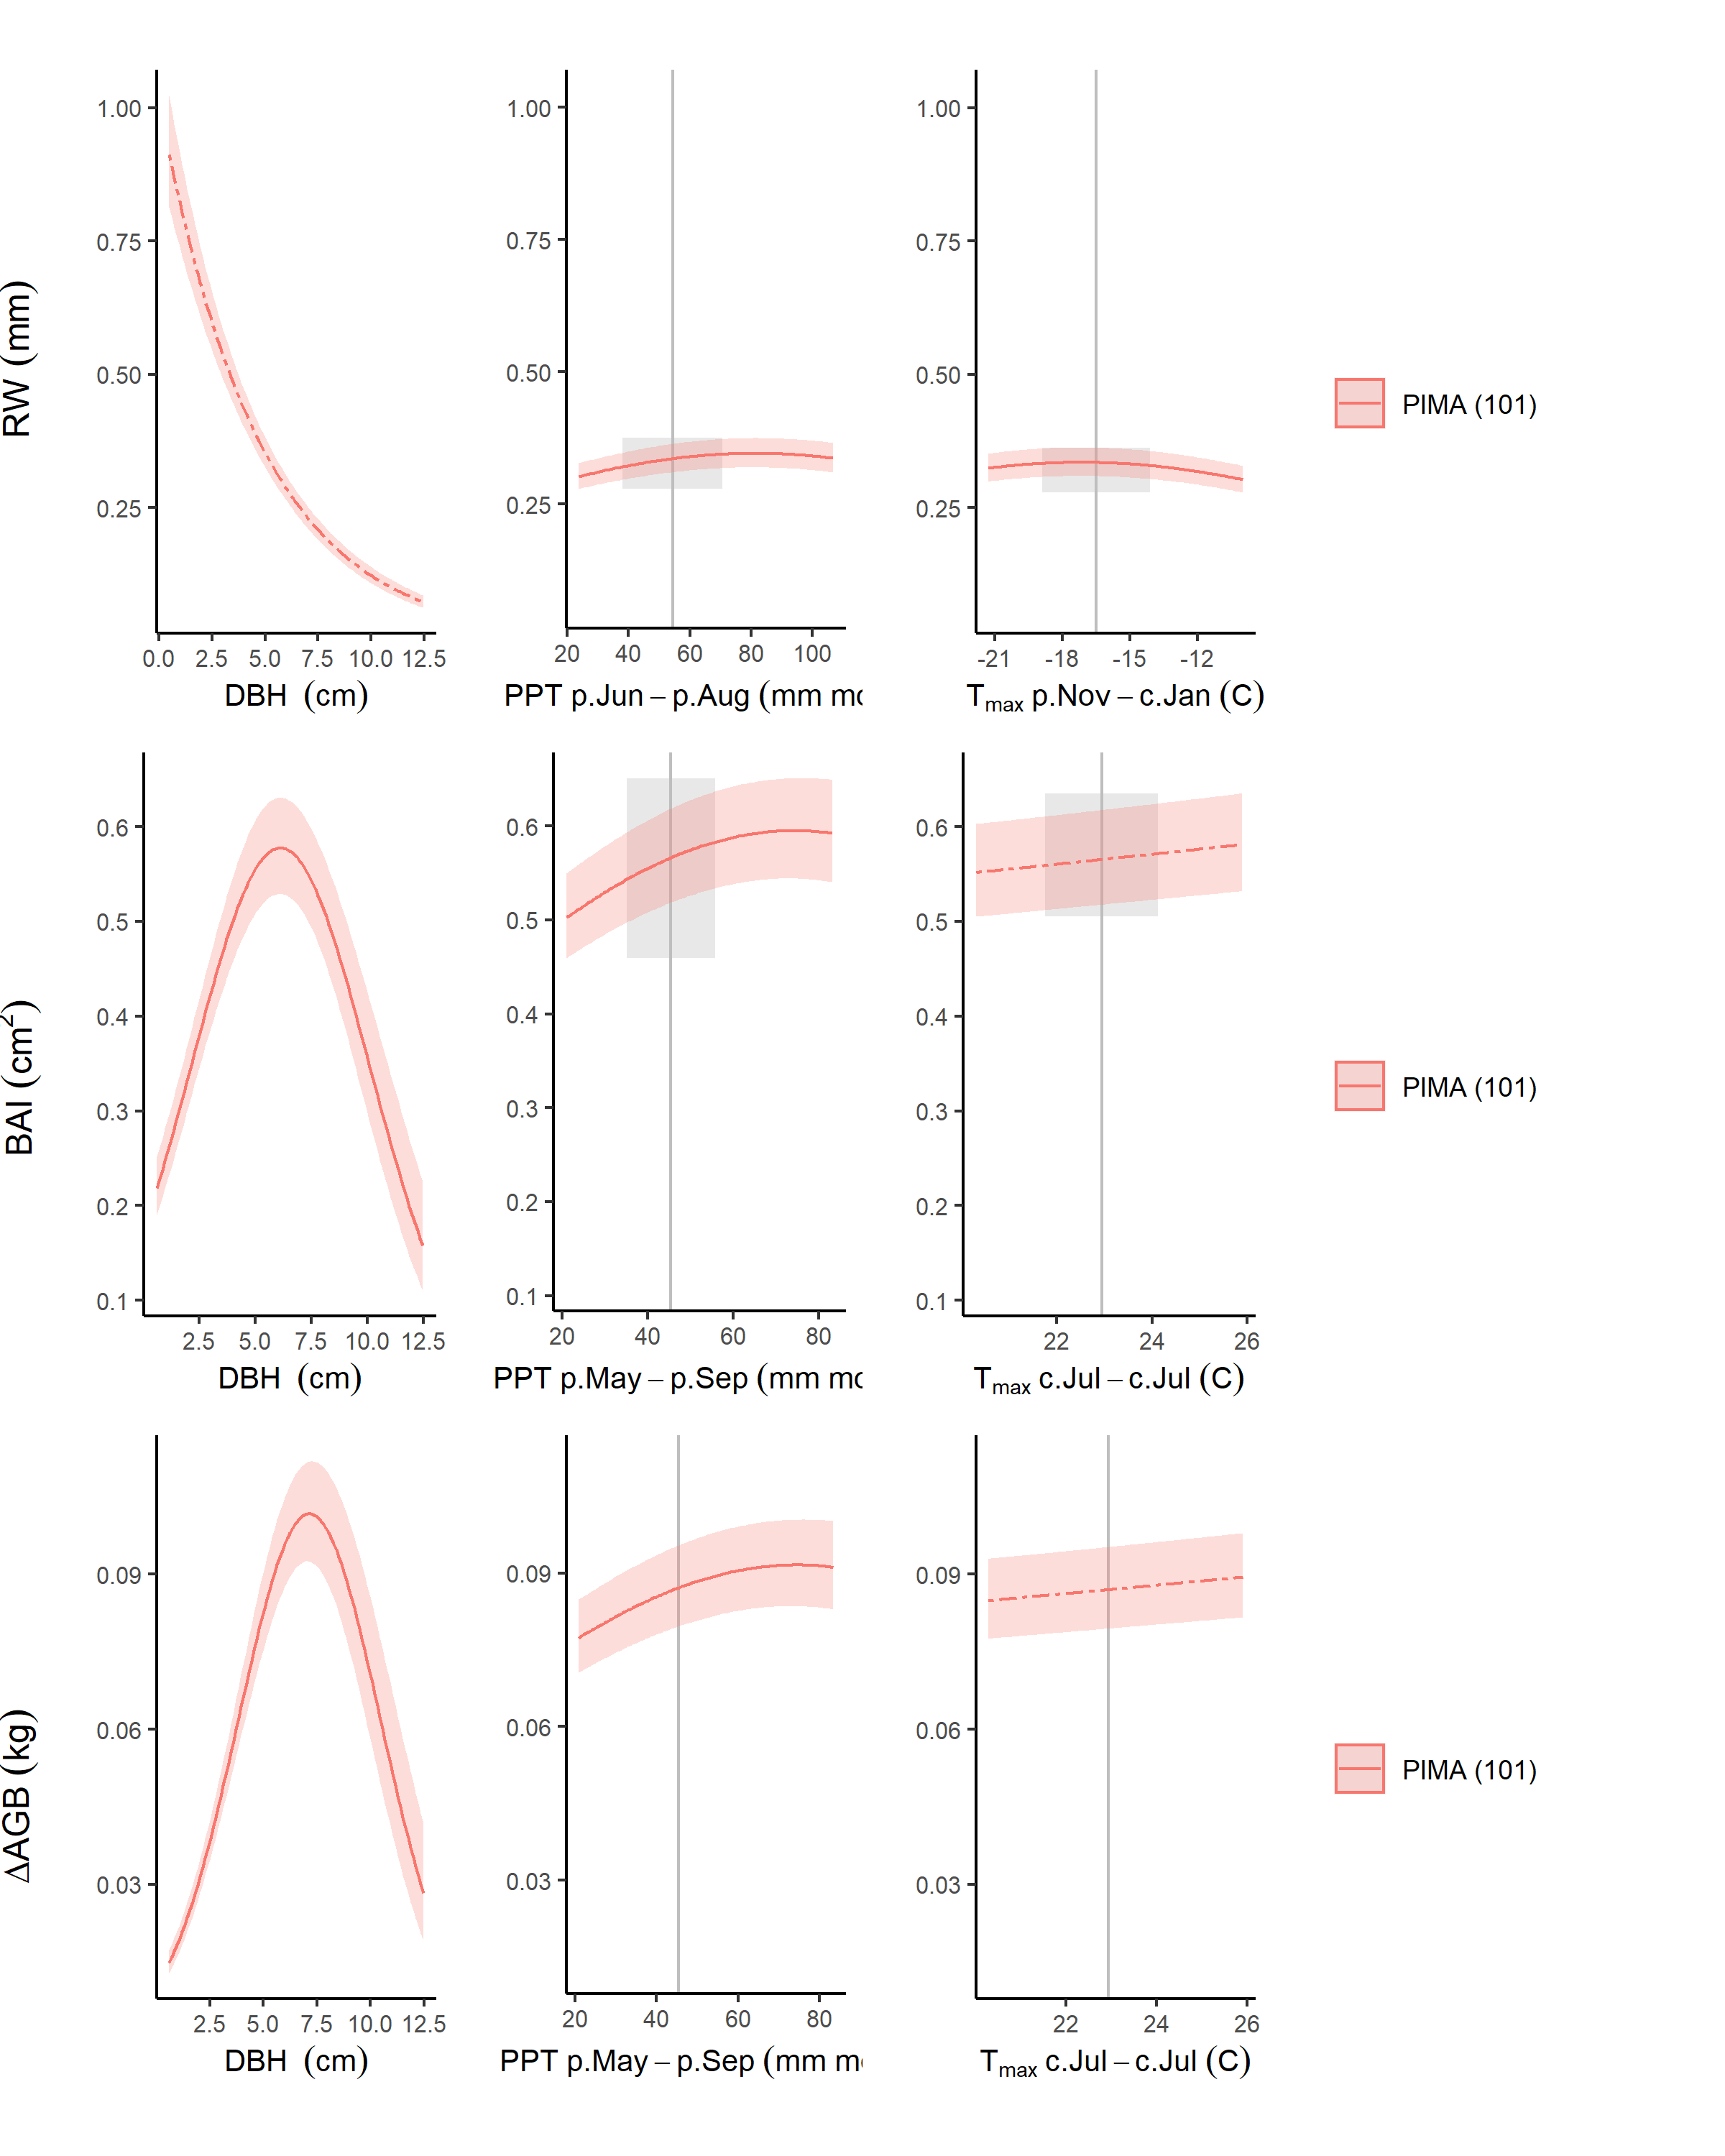
\includegraphics[width=0.75\textwidth,height=\textheight]{tables_figures/SI_figures/composite_plots/ScottyCreek.png}
\caption{Figure S18. Best GLS models for Scotty Creek (Northwest
Territory, Canada) for all three growth metrics examined here.
Precipitation and temperature group variables are as selected by
\emph{climwin} (p=previous year, c=current year). For each species,
relationships are plotted if included in top model, with best-fit
polynomials plotted with solid lines when both first- and second-order
terms are signficant, dashed lines when only one term is signficant, and
dotted lines when neither is signficant. Transparent ribbons indicate
95\% confidence intervals. Vertical grey lines indicate the long-term
mean for the climate variable, shading indicates 1 SD.}
\end{figure}

\newpage

\hypertarget{si-references}{%
\subsection*{SI References}\label{si-references}}
\addcontentsline{toc}{subsection}{SI References}

\hypertarget{refs}{}
\begin{cslreferences}
\leavevmode\hypertarget{ref-applequist_simple_1958}{}%
Applequist, M. (1958). A simple pith locator for use with off-center
increment cores. \emph{Journal of Forestry}.

\leavevmode\hypertarget{ref-aus_de_ar_tree_2018}{}%
Aus de Ar, R. (2018). Tree Rings of Pinus ponderosa and Juniperus
virginiana Show Different Responses to Stand Density and Water
Availability in the Nebraska Grasslands. \emph{The American Midland
Naturalist}, \emph{180}(1), 18.
doi:\href{https://doi.org/10.1674/0003-0031-180.1.18}{10.1674/0003-0031-180.1.18}

\leavevmode\hypertarget{ref-bumann_assessing_2019}{}%
Bumann, E., Awada, T., Wardlow, B., Hayes, M., Okalebo, J., Helzer, C.,
\ldots{} Cherubini, P. (2019). Assessing responses of \emph{Betula}
\emph{Papyrifera} to climate variability in a remnant population along
the Niobrara River Valley in Nebraska, U.S.A., Through dendroecological
and remote-sensing techniques. \emph{Canadian Journal of Forest
Research}, \emph{49}(5), 423--433.
doi:\href{https://doi.org/10.1139/cjfr-2018-0206}{10.1139/cjfr-2018-0206}

\leavevmode\hypertarget{ref-charney_observed_2016}{}%
Charney, N. D., Babst, F., Poulter, B., Record, S., Trouet, V. M.,
Frank, D., \ldots{} Evans, M. E. K. (2016). Observed forest sensitivity
to climate implies large changes in 21st century North American forest
growth. \emph{Ecology Letters}, \emph{19}(9), 1119--1128.
doi:\href{https://doi.org/10.1111/ele.12650}{10.1111/ele.12650}

\leavevmode\hypertarget{ref-duncan_evaluation_1989}{}%
Duncan, R. P. (1989). An evaluation of errors in tree age estimates
based on increment cores in kahikatea (Dacrycarpus dacrydioides).
\emph{New Zealand Natural Sciences}, \emph{16}, 31--37.

\leavevmode\hypertarget{ref-helcoski_growing_2019}{}%
Helcoski, R., Tepley, A. J., Pederson, N., McGarvey, J. C., Meakem, V.,
Herrmann, V., \ldots{} Anderson-Teixeira, K. J. (2019). Growing season
moisture drives interannual variation in woody productivity of a
temperate deciduous forest. \emph{New Phytologist}, \emph{223}(3),
1204--1216.
doi:\href{https://doi.org/10.1111/nph.15906}{10.1111/nph.15906}

\leavevmode\hypertarget{ref-kaspar_species-specific_nodate}{}%
Kašpar, K., Tumajer, J., Vašíčková, I., \& Šamonil, P. (n.d.).
Species-specific climate-growth interactions determine the future tree
species dynamics of the mixed Central European mountain forests.

\leavevmode\hypertarget{ref-maxwell_declining_2016}{}%
Maxwell, J. T., Harley, G. L., \& Robeson, S. M. (2016). On the
declining relationship between tree growth and climate in the Midwest
United States: The fading drought signal. \emph{Climatic Change},
\emph{138}(1-2), 127--142.
doi:\href{https://doi.org/10.1007/s10584-016-1720-3}{10.1007/s10584-016-1720-3}

\leavevmode\hypertarget{ref-paton_barro_2019}{}%
Paton, S. (2019, October). Barro Colorado Island,
Clearing\_Precipitation, manual. The Smithsonian Institution.
doi:\href{https://doi.org/10.25573/data.10042502.v3}{10.25573/data.10042502.v3}

\leavevmode\hypertarget{ref-sniderhan_growth_2016}{}%
Sniderhan, A. E., \& Baltzer, J. L. (2016). Growth dynamics of black
spruce ( \emph{Picea} \emph{Mariana} ) in a rapidly thawing
discontinuous permafrost peatland: Growth Dynamics Boreal Peatlands.
\emph{Journal of Geophysical Research: Biogeosciences}, \emph{121}(12),
2988--3000.
doi:\href{https://doi.org/10.1002/2016JG003528}{10.1002/2016JG003528}

\leavevmode\hypertarget{ref-tumajer_increasing_2017}{}%
Tumajer, J., Altman, J., Štěpánek, P., Treml, V., Doležal, J., \&
Cienciala, E. (2017). Increasing moisture limitation of Norway spruce in
Central Europe revealed by forward modelling of tree growth in tree-ring
network. \emph{Agricultural and Forest Meteorology}, \emph{247}, 56--64.
doi:\href{https://doi.org/10.1016/j.agrformet.2017.07.015}{10.1016/j.agrformet.2017.07.015}

\leavevmode\hypertarget{ref-vlam_temperature_2014}{}%
Vlam, M., Baker, P. J., Bunyavejchewin, S., \& Zuidema, P. A. (2014).
Temperature and rainfall strongly drive temporal growth variation in
Asian tropical forest trees. \emph{Oecologia}, \emph{174}(4),
1449--1461.
doi:\href{https://doi.org/10.1007/s00442-013-2846-x}{10.1007/s00442-013-2846-x}

\leavevmode\hypertarget{ref-williams_temperature_2012}{}%
Williams, A. P., Allen, C. D., Macalady, A. K., Griffin, D., Woodhouse,
C. A., Meko, D. M., \ldots{} McDowell, N. G. (2012). Temperature as a
potent driver of regional forest drought stress and tree mortality.
\emph{Nature Climate Change}.
doi:\href{https://doi.org/10.1038/nclimate1693}{10.1038/nclimate1693}
\end{cslreferences}

\end{document}
